\documentclass{article}

  % packages
    % basic stuff for rendering math
    \usepackage[letterpaper, top=1in, bottom=1in, left=1in, right=1in]{geometry}
    \usepackage[utf8]{inputenc}
    \usepackage[english]{babel}
    \usepackage{amsmath} 
    \usepackage{amssymb}
    % \usepackage{amsthm}

    % extra math symbols and utilities
    \usepackage{mathtools}        % for extra stuff like \coloneqq
    \usepackage{mathrsfs}         % for extra stuff like \mathsrc{}
    \usepackage{centernot}        % for the centernot arrow 
    \usepackage{bm}               % for better boldsymbol/mathbf 
    \usepackage{enumitem}         % better control over enumerate, itemize
    \usepackage{xr-hyper}
    \usepackage{hyperref}         % for hypertext linking
    \usepackage{fancyvrb}          % for better verbatim environments
    \usepackage{newverbs}         % for texttt{}
    \usepackage{xcolor}           % for colored text 
    \usepackage{listings}         % to include code
    \usepackage{lstautogobble}    % helper package for code
    \usepackage{parcolumns}       % for side by side columns for two column code
    

    % page layout
    \usepackage{fancyhdr}         % for headers and footers 
    \usepackage{lastpage}         % to include last page number in footer 
    \usepackage{parskip}          % for no indentation and space between paragraphs    
    \usepackage[T1]{fontenc}      % to include \textbackslash
    \usepackage{footnote}
    \usepackage{etoolbox}

    % for custom environments
    \usepackage{tcolorbox}        % for better colored boxes in custom environments
    \tcbuselibrary{breakable}     % to allow tcolorboxes to break across pages

    % figures
    \usepackage{pgfplots}
    \pgfplotsset{compat=1.18}
    \usepackage{float}            % for [H] figure placement
    \usepackage{tikz}
    \usepackage{tikz-cd}
    \usepackage{circuitikz}
    \usetikzlibrary{arrows}
    \usetikzlibrary{positioning}
    \usetikzlibrary{calc}
    \usepackage{graphicx}
    \usepackage{algorithmic}
    \usepackage{caption} 
    \usepackage{subcaption}
    \captionsetup{font=small}

    % for tabular stuff 
    \usepackage{dcolumn}

    \usepackage[nottoc]{tocbibind}
    \pdfsuppresswarningpagegroup=1
    \hfuzz=5.002pt                % ignore overfull hbox badness warnings below this limit

  % New and replaced operators
    \DeclareMathOperator*{\card}{card}
    \DeclareMathOperator{\im}{Im}
    \DeclareMathOperator{\re}{Re}
    \DeclareMathOperator*{\argmin}{\arg\!\min}
    \DeclareMathOperator*{\argmax}{\arg\!\max}
    \newcommand{\qed}{\hfill$\blacksquare$}     % I like QED squares to be black

  % Custom Environments
    \tcbset{
      colframe = black,
      colback  = white,
      coltitle = black,
      colbacktitle = black!10,
      breakable, 
      arc=0mm,
      boxrule=1pt,
      left=8pt,
      right=8pt,
      top=6pt,
      bottom=6pt,
      before skip=12pt,
      after skip=12pt,
      bottomrule at break=-1pt,
      toprule at break=-1pt,
      fonttitle=\bfseries,
    }
    \newtcolorbox[auto counter, number within=section]{question}[1][]
    {
      title = \textbf{Question \thetcbcounter ~(#1)}
    }
    \newtcolorbox[auto counter, number within=section]{axiom}[1][]
    {
      title = \textbf{Axiom \thetcbcounter ~(#1)}
    }
    \newtcolorbox[auto counter, number within=section]{exercise}[1][]
    {
      title = \textbf{Exercise \thetcbcounter ~(#1)}
    }
    \newtcolorbox[auto counter, number within=section]{solution}[1][]
    {
      title = \textbf{Solution \thetcbcounter}
    }
    \newtcolorbox[auto counter, number within=section]{lemma}[1][]
    {
      title = \textbf{Lemma \thetcbcounter ~(#1)},
    }
    \newtcolorbox[auto counter, number within=section]{theorem}[1][]
    {
      title = \textbf{Theorem \thetcbcounter ~(#1)},
    } 
    \newtcolorbox[auto counter, number within=section]{corollary}[1][]
    {
      title = \textbf{Corollary \thetcbcounter ~(#1)},
    } 
    \newtcolorbox[auto counter, number within=section]{proof}[1][]
    {
      before skip = -7pt,
      before upper = \textit{Proof. },
    } 
    \newtcolorbox[auto counter, number within=section]{definition}[1][]
    {
      title = \textbf{Definition \thetcbcounter ~(#1)}
    }
    \newtcolorbox[auto counter, number within=section]{example}[1][]
    {
      title = \textbf{Example \thetcbcounter ~(#1)}
    } 
    \newtcolorbox[auto counter, number within=section]{code}[1][]
    {
      title = \textbf{Code \thetcbcounter ~(#1)}
    } 

    \definecolor{dkgreen}{rgb}{0,0.6,0}
    \definecolor{gray}{rgb}{0.5,0.5,0.5}
    \definecolor{mauve}{rgb}{0.58,0,0.82}
    \definecolor{lightgray}{gray}{0.93}

    % default options for listings (for code)
    \lstset{
      autogobble,
      frame=ltbr,
      language=C,                           % the language of the code
      aboveskip=3mm,
      belowskip=3mm,
      showstringspaces=false,
      columns=fullflexible,
      keepspaces=true,
      basicstyle={\small\ttfamily},
      numbers=left,
      firstnumber=1,                        % start line number at 1
      numberstyle=\tiny\color{gray},
      keywordstyle=\color{blue},
      commentstyle=\color{dkgreen},
      stringstyle=\color{mauve},
      backgroundcolor=\color{lightgray}, 
      breaklines=true,                      % break lines
      breakatwhitespace=true,
      tabsize=3, 
      xleftmargin=2em, 
      framexleftmargin=1.5em, 
      stepnumber=1
    }

  % Page style
    \pagestyle{fancy}
    \fancyhead[L]{Set Theory}
    \fancyhead[C]{Muchang Bahng}
    \fancyhead[R]{Spring 2025} 
    \fancyfoot[C]{\thepage / \pageref{LastPage}}
    \renewcommand{\footrulewidth}{0.4pt}          % the footer line should be 0.4pt wide
    \renewcommand{\thispagestyle}[1]{}  % needed to include headers in title page

  % external documents 
    \externaldocument[place-]{../Point_Set_Topology/paper}[../Point_Set_Topology/paper.pdf] 
    \externaldocument[place-]{../Real_Analysis/paper}[../Real_Analysis/paper.pdf] 

\begin{document}

\title{ZFC Set Theory}
\author{Muchang Bahng}
\date{Spring 2025}

\maketitle
\tableofcontents
\pagebreak

Unlike my machine learning notes, which focuses mostly on the theoretical soundness of classical (e.g. pre-deep and interpretable) models, the theory of deep neural networks have not been developed as well yet. Furthermore, the recency of developments, especially in the post-2010s, results in a pretty nonlinear\footnote{No pun intended.} timeline that is difficult to categorize effectively. Before I give my motivation, the direct prerequisites for deep learning are basic knowledge of my notes in probability theory, machine learning, and real analysis. 

Therefore, after much thought, I think organizing my notes in chronological order would be best. It turned out that in the early days of deep learning, most researchers like Andrew Ng stated that he focused on supervised models,\footnote{He states this in his podcast with Lex Fridman.} and it wasn't until the 2010s that the development of unsupervised models burgeoned. 

\begin{enumerate}
  \item We start by introducing \textit{multilayered perceptrons} (MLPs), which build upon generalized linear models (GLMs) that we have went over in machine learning. This is pretty much the ``foundational'' model that we will build on. We then talk a about practical methodologies regarding training and control. 

  \item Then we introduce the other two architectures. The \textit{convolutional neural network} (CNN) gives us a scalable way to perform sparse matrix multiplication efficiently, by taking advantage of locality. Then in \textit{recurrent neural networks} (RNNs), we are not limited to a single $n$-dimensional vector input and are able to process a time series of inputs.  
    
  \item With these building blocks, we are able take and two neural networks together to create an encoder-decoder model. The two main applications of this was dimensionality reduction with \textit{autoencoders}, followed by \textit{seq2seq} for machine translation between sequences of words.  

  \item The practical success of autoencoders led to the development of not just density estimation models, but \textit{generative} ones that seek to sample from the learned distribution. These generative models were ``deep'' extensions of the classical linear factor models resulting in \textit{restricted Boltzmann machines (RBMs)} and \textit{variational autoencoders (VAEs)}, which attempted to explicitly model an approximation of the true data generating distribution. More specifically, RBMs were \textit{energy models} that borrowed ideas from physics to learn a distribution of the form $p_X (x) = \frac{1}{Z} e^{-f_\theta (x)}$. To sample from this, researchers already had access to the established Markov Chain Monte Carlo (MCMC) algorithms designed for this exact problem. As for VAEs, these were trained and sampled through \textit{variational inference} methods. 

  \item In 2014, a completely new architecture composed of 2 neural networks competing each other gave rise to \textit{generative adversarial networks} (GANs) which blew RBMs and VAEs away. A similar architecture followed with \textit{generative stochastic networks} (GSNs).

  \item In 2016, \textit{normalizing flow models}, which attempted to model a smooth function that transformed simple latent variables to the true data generating distribution, were invented by Google DeepMind and surpassed GANs. 

  \item In 2017, \textit{attention} took the world by storm, which had drastically improved machine translation in seq2seq, and the resulting \textit{self-attention} plus the \textit{transformer} architectures led to the success of OpenAI's ChatGPT. 
\end{enumerate} 

Again, I emphasize that the math in these notes are not very advanced. However, implementing these simple models and training algorithms from scratch is a challenge in itself. I will go through implementing everything from scratch as if we were building a mini-version of PyTorch as we learn new topics. My implementations can be found \href{https://github.com/mbahng/pyember}{here}. 

\section{Sets} 

  So with these paradoxes in mind, we would like to construct an axiomatic formulation of sets. My take is to think that sets ``exist'' out there somewhere in the universe, and our job is to find them. Cantor with his naive set theory believed that for every meaningful property of things there is a set whose members are exactly all the things with that property. Russell shows this this cannot be the case. Nevertheless, \textit{some} sets exist, and we have intuitive experience thinking about finite sets. Therefore, the axioms of set theory are a limited list of \textit{assumptions} that we hope are true about that actually existing universe of sets. As long as they are true, then whatever we conclude from them by valid reasoning steps must also be true.\footnote{This idea is called naive Platonism.} Hence we have the following definition, which first requires the familiar property of acting like a collection of something, and then obeys the axioms we set. 
  
  \begin{definition}[Set]
    A \textbf{set} $X$ is anything 
    \begin{enumerate}
      \item that has the innate property of containing elements, and 
      \item obeys the axioms of ZF(C). 
    \end{enumerate}
  \end{definition}  

  Let's first talk about the language, where they are defined formally using the axioms in the next subsection. From first-order logic, note that we have the following symbols in our alphabet $\mathcal{L}_{\mathrm{ZFC}}$. 
  \begin{enumerate}
    \item The logical connectives $\neg$, $\lor$, $\land$. 
    \item The quantifier symbols $\exists, \forall$ 
    \item Brackets $()$. 
  \end{enumerate}
  To represent sets, we also need symbols, and the membership property requires us to define a symbol for that too. 
  \begin{enumerate}
    \item A countably infinite amount of variables used for representing sets. 
    \item The set membership symbol $\in$. In fact, when we say $x \in A$, this is a proposition formed from the predicate $P(x)$. 
  \end{enumerate} 
  This is what we have to work with so far. We will construct the rest of the symbols ($=, \subset, \supset, \cup, \cap$) from the axioms. 

  Now we state the axioms, which is the foundation of ZF set theory. A question one might ask is: how do we even know for sure that these axioms aren't contradictory? The answer is that we don't, and that is why we take them as axioms rather than provable theorems. Fortunately, from the formulation in the early 20th century up until now, no contradictions have been found, and if there is one, then it would be very bad news for us.  
  
  As obvious as the axioms may seem, none of them can be rigorously proven since we need to start from a set of assumptions and some principles of logic to use some deductive reasoning. 

  \begin{axiom}[Axiom of Existence]
    There exists a set which has no elements.\footnote{Technically, this does not need to be stated as an axiom, but it is often done for convenience. Indeed, by the axiom of infinity, there exists some set $S$. By the axiom of restricted comprehension, we can define $\{x \in S \mid x \neq x\}$, which is empty since the predicate always evaluates to false. }
  \end{axiom}

  \begin{definition}[Empty Set]
    The \textbf{empty set} is denoted $\emptyset$.\footnote{Note that this is not determined to be unique... yet!} 
  \end{definition}

  Why do we need to axiomize what seems to be such an obvious thing? The rest of the axioms that follow talk about what we can or cannot do with sets, but this whole theory would be useless if we didn't know if there exists \textit{any} set that obeys the following axioms! Therefore, we would like to assert the existence of at least one set, namely the empty set. This asserts that our universe of discourse is not void, and so it gives us a starting set to work with, which we can build on to create more sets.   

\subsection{Axiom of Extensionality} 

  The empty set is simply described as the set containing nothing, but it can be constructed in various ways. I can describe it as the set of humans that have negative age, or the set of married bachelors. All examples of this kind describe one and the same set $\emptyset$, but we cannot yet prove this. This is why we need our second axiom, which states that a set is uniquely characterized simply by its elements. 

  \begin{axiom}[Axiom of Extensionality]
    Two sets are equal (are the same set) if they have the same elements. 
    \begin{equation}
      \forall A \forall B \big[ \forall x (x \in A \iff x \in B) \iff A = B\big]
    \end{equation}
  \end{axiom} 

  \begin{definition}[Equality]
    This axiom allows us to define the equality operator $=$, which we now add to our alphabet. 
  \end{definition} 

  \begin{theorem}[Uniqueness of Empty Set]
    The empty set is unique. 
  \end{theorem}
  \begin{proof}
    Assume that $A$ and $B$ are sets with no elements. Then it is vacuously true that every element of $A$ is an element of $B$, and vice versa. Therefore by the axiom of extensionality $A = B$. 
  \end{proof}

  This next theorem now shows that every set is uniquely characterized by its distinct elements, which aligns with our established notion that sets don't contain repeated elements. 

  \begin{theorem}[Sets Don't Contain Repeated Elements]
    Sets are unique up to distinct elements. That is, given 2 sets $A, B$, 
    \begin{equation}
      \forall x (x \in A \iff x \in B) \implies A = B
    \end{equation}
  \end{theorem} 

  As an example, we have the following: 
  \begin{equation}
    \{1, 1, 2\} = \{1, 2\} = \{1, 1, 2, 2\}
  \end{equation} 
  Though note that we don't even know if any of the sets above even exist with our axioms so far! 

\subsection{Axiom of Restricted Comprehension}

  The axiom assists us in regulating which sets are viable and which are not, preventing Russell's paradox. 

  \begin{axiom}[Axiom Schema of Restricted Comprehension]
    Given $P$ a formula with $P(x)$ specifying a property of $x$, for any set $A$, there exists a set $B$ such that $x \in B$ if and only if $x \in A$ and $P(x)$. That is, if $A$ exists, then the set, written in set-builder notation, 
    \begin{equation}
      B = \{x \in A \mid P(x) \}
    \end{equation}
    exists.\footnote{Note that this axiom does not allow the construction of entities of the more general form $\{x \mid P(x)\}$. This restriction is obviously needed to avoid Russell's paradox, hence the name \textit{restricted} comprehension. } 
  \end{axiom} 

  \begin{lemma}[Uniqueness of Restricted Commprehension]
    The set $B = \{x \in A \mid P(x) \}$ is unique, and therefore it makes sense to treat it as a unique object. 
  \end{lemma}

  The axiom of specification allows us to denote subsets. 

  \begin{definition}[Subset, Superset]
    Notationally, if $A$ is a subset of $B$, then we write $A \subset B$. Similarly, we say $A$ is a \textbf{superset} of $B$, written $A \supset B$, if $B \subset A$. 
  \end{definition} 

  We can extend this to the restriction of more sets. 

  \begin{theorem}[Existence of Binary Intersection]
    That is, if $A, B$ are sets, then there is a set $C$ such that $x \in C$ if and only if $x \in A$ and $x \in B$. This allows us to define intersection as 
    \begin{equation}
      A \cap B \coloneqq \{x \in A \mid x \in B \}
    \end{equation} 
  \end{theorem} 
  \begin{proof}
    
  \end{proof} 

  We can extend this proof to define the intersection of a set of sets. 
  
  \begin{definition}[Intersection]
    Given a nonempty\footnote{$\cap \emptyset$ is not defined since every $x$ belongs to all $A \in \emptyset$ vacuously, and so such a set would be the universal set, which does not exist.} set of sets $S$, the \textbf{intersection} $\cap S$ is the unique set satisfying $x \in \cap S$ if and only if $x \in A$ for all $A \in S$. In set builder notation, we can write 
    \begin{equation}
      \bigcap S \coloneqq \{x \in A \mid \forall B (B \in S \implies x \in B) \}
    \end{equation}
    We can also expand our notation by defining the following. 
    \begin{enumerate}
      \item Just another way of writing is 
        \begin{equation}
          \cup S = \bigcap_{A \in S} A
        \end{equation}

      \item By the axiom of extensionality, we can define 
        \begin{equation}
          A_1 \cap \ldots \cap A_n = \cap \{A_1, \ldots, A_n\}
        \end{equation}
    \end{enumerate}
  \end{definition}

  \begin{definition}[Disjoint Sets]
    Two sets $A$ and $B$ are \textbf{disjoint} if $A \cap B = \emptyset$. 
  \end{definition}

  Unfortunately, the union cannot be expressed in this specification schema, and we need a separate axiom for this. 

  \begin{definition}[Set Minus]
    We can however define set minus. Given sets $A, B$
    \begin{equation}
      A \setminus B \coloneqq \{ x \in A \mid x \not\in B \}
    \end{equation}
  \end{definition}

  \begin{definition}[Set Complement]
    Given $B$ and a subset $A \subset B$, the \textbf{complement} of $A$ with respect to $B$ is 
    \begin{equation}
      A^c \coloneqq \{ x \in B \mid x \not\in A \} = B \setminus A
    \end{equation}
  \end{definition}  

  \begin{definition}[Symmetric Difference]
    Given sets $A, B$, the \textbf{symmetric difference} between the two sets is defined 
    \begin{equation}
      A \triangle B \coloneqq (A \setminus B) \cup (B \setminus A)
    \end{equation}
  \end{definition} 

\subsection{Axiom of Pairing}

  Okay this is all great, but the only set that we have claimed the existence of is $\emptyset$, and the schema of restricted comprehension is useless in constructing any new sets since 
  \begin{equation}
    \{x \in \emptyset \mid P(x) \} = \emptyset
  \end{equation}
  for any property $P$. Starting from now, we provide more helpful axioms to construct new sets. 

  \begin{axiom}[Axiom of Pairing]
    If $A, B$ are sets, then there exists a set which contains $A$ and $B$ as elements.\footnote{For example, if $A = \{1, 2\}$ and $B = \{2, 3\}$,then $\{\{1, 2\}, \{2, 3\}\}$ exists.}
    \begin{equation}
      \forall A \forall B \exists C((A \in C) \land (B \in C))
    \end{equation}
    This allows us to construct sets from old ones. 
  \end{axiom}

  Note that clearly, this set is not necessarily unique, since there can be other elements in $C$ in addition to $A$ and $B$. 

  \begin{theorem}[Nested Sets]
    By the axiom of pairing, if we have a set $X$, then $\{X\}$ is also a set, since we can set $A = B = X$ which asserts the existence of $\{X, X\} = \{X\}$. 
  \end{theorem} 

  \begin{example}[More Sets]
    Now we have unlocked our first sets that are not the empty set! Consider the following. 
    \begin{enumerate}
      \item If $A = B = \emptyset$, then by the axiom of pairing we can get $C = \{\emptyset, \emptyset\}$, which is equal to $\{\emptyset\}$ by the axiom of extensionality. 
      \item Now we let $A = \emptyset, B = \{\emptyset\}$, and so $C = \{A, B \} = \{\emptyset, \{\emptyset\}\}$. 
    \end{enumerate}
  \end{example}

\subsection{Axiom of Union}

  \begin{axiom}[Axiom of Union] 
    For any set of sets $S$, there exists a set $U$ such that $x \in U$ if and only if $x \in A$ for some $A \in S$. 
    \begin{equation}
      \forall \mathcal{F} \exists U \forall X \forall x \big[ (x \in X \land X \in \mathcal{F}) \implies x \in U \big]
    \end{equation}
  \end{axiom}

  \begin{lemma}[Union is Unique]
    The union $U$ is unique. 
  \end{lemma}
  \begin{proof}
    Again use the axiom of extensionality. 
  \end{proof} 

  \begin{definition}[Union]
    The set $U$, is called the \textbf{union} of sets $A \in S$, denoted $\cup S$. We can also expand our notation by defining the following. 
    \begin{enumerate}
      \item Just another way of writing is 
        \begin{equation}
          \cup S = \bigcup_{A \in S} A
        \end{equation}

      \item By the axiom of extensionality, we can define 
        \begin{equation}
          A_1 \cup \ldots \cup A_n = \cup \{A_1, \ldots, A_n\}
        \end{equation}
    \end{enumerate}
  \end{definition}

  Sometimes, it is formulated alternatively as follows: For any set of sets $S$, there is a set $U$ containing every element that is a member of $S$. This does not necessarily mean that $U$ is unique, and so $\cup S$ is not defined yet. However, we can define it by using the axiom of restricted comprehension and defining 
  \begin{equation}
    \cup S \coloneqq \{ x \in A \mid \exists X (x \in X \land X \in S ) \}
  \end{equation}

  \begin{example}
    \begin{equation}
      \{\{\emptyset\}\} \cup \{\emptyset, \{\emptyset\}\} = \{\emptyset, \{\emptyset\}\}
    \end{equation}
  \end{example}

\subsection{Rules of Set Operations}

  Let's first talk about rules following the union, intersection, and set minus operators. 

  \begin{theorem}[Commutativity]
    Union and intersection are commutative. 
    \begin{align}
      A \cup B & = B \cup A \\
      A \cap B & = B \cap A
    \end{align}
  \end{theorem}

  \begin{theorem}[Associativity]
    Union and intersection are associative. 
    \begin{align}
      (A \cup B) \cup C & = A \cup (B \cup C) \\
      (A \cap B) \cap C & = A \cap (B \cap C) 
    \end{align}
  \end{theorem}

  \begin{theorem}[Distributivity]
    Given sets $A, B, C$, 
    \begin{align}
      A \cap (B \cup C) & = (A \cap B) \cup (A \cap C) \\
      A \cup (B \cap C) & = (A \cup B) \cap (A \cup C)
    \end{align}
  \end{theorem}
  \begin{proof}
    Listed. 
    \begin{enumerate}
      \item $A \cap (B \cup C) = (A \cap B) \cup (A \cap C)$. 
        \begin{enumerate}
          \item $A \cap (B \cup C) \subset (A \cap B) \cup (A \cap C)$. Assume $x \in A \cap (B \cup C)$. Then $x \in A$ and $x \in B \cup C$. If $x \in B$, then $x \in A \cap B$. If $x \in C$, then $x \in A \cap C$. Therefore, since $x \in B \cup C$, it must be the case that $x \in A \cap B$ or $x \in A \cap C$, which by definition implies $x \in (A \cap B) \cup (A \cap C)$. 

          \item $A \cap (B \cup C) \supset (A \cap B) \cup (A \cap C)$. Assume that $x \in (A \cap B) \cup (A \cap C)$. Then WLOG let $x \in A \cap B$. Then $x \in A$ and $x \in B \subset (B \cup C)$, so by definition $x \in A \cap (B \cup C)$. 
        \end{enumerate}

      \item $A \cup (B \cap C) = (A \cup B) \cap (A \cup C)$.
        \begin{enumerate}
          \item $A \cup (B \cap C) \subset (A \cup B) \cap (A \cup C)$. Assume $x \in A \cup(B \cap C)$. Then $x \in A$ or $x \in B \cap C$. If $x \in A$, then since $A \subset (A \cup B)$ and $A \subset (A \cup C)$, we have $x \in (A \cup B)$ and $x \in (A \cup C)$, which by definition means $x \in (A \cup B) \cap (A \cup C)$. If $x \not\in A$, then $x \in B \cap C \implies x \in B \subset (A \cup B)$ and $x \in C \subset (A \cup C)$, and so $x \in (A \cup B) \cap (A \cup C)$. 

          \item $A \cup (B \cap C) \supset (A \cup B) \cap (A \cup C)$. Assume $x \in (A \cup B) \cap (A \cup C)$. Then $x \in A \cup B$. If $x \in A$, then since $A \subset A \cup (B \cap C)$, $x \in A \cup (B \cap C)$. If $x \not\in A$, then $x \in B$. Since $x \in A \cup C$, $x \in C$ also. Therefore by definition $x \in (B \cap C) \subset A \cup (B \cap C) \implies x \in A \cup (B \cap C)$. 
        \end{enumerate}
    \end{enumerate}
  \end{proof}

  \begin{theorem}[DeMorgan's Laws]
    If $X$ is a set and $A, B \subset X$, then 
    \begin{align}
      X \setminus (A \cup B) & = (X \setminus A) \cap (X \setminus B) \\
      X \setminus (A \cap B) & = (X \setminus A) \cup (X \setminus B)
    \end{align}
  \end{theorem}
  \begin{proof}
    Listed. 
    \begin{enumerate}
      \item $X \setminus (A \cup B) = (A \setminus A) \cap (X \setminus B)$.
        \begin{enumerate}
          \item $X \setminus (A \cup B) \subset (A \setminus A) \cap (X \setminus B)$. Assume $x \in X \setminus (A \cup B) \iff x \in X$ and $x \not\in (A \cup B)$. Since $x \not\in (A \cup B$, $x \not\in A$ and $x \not\in B$. However, $x \in X$, so $x \not\in A \implies x \in X \setminus A$. Same goes for $B$, and so $x \in (X \setminus A) \cap (X \setminus B)$. 

          \item $X \setminus (A \cup B) \supset (A \setminus A) \cap (X \setminus B)$. Assume $x \in (X \setminus A) \cap (X \setminus B)$. Then $x \in X \setminus A \iff X \in X$ and $x \not\in A$, and $x \in X \setminus B \iff x \in X$ and $x \not\in B$. Since $x \not\in A$ and $x \not\in B$, $x \not\in A \cup B$. Combined with the fact that $x \in X$, we have $x \in X \setminus (A \cup B)$. 
        \end{enumerate}

      \item $X \setminus (A \cap B) = (A \setminus A) \cup (X \setminus B)$.
        \begin{enumerate}
          \item $X \setminus (A \cap B) \subset (A \setminus A) \cup (X \setminus B)$. Let $x \in X \setminus (A \cap B)$. Then $x \in X$ and $x \not\in A \cap B$. Since $x \not\in A \cap B$, it must be the case that at least $x \not\in A$ or $x \not\in B$. WLOG let $x \not\in A$. Then $x \in X$ and $x \not\in A \implies x \in (X \setminus A) \subset (X \setminus) \cup (X \setminus B) \implies x \in (X \setminus A) \cup (X \setminus B)$. 

          \item $X \setminus (A \cap B) \supset (A \setminus A) \cup (X \setminus B)$. WLOG let $x \in (X \setminus A)$. Then $x \in X$ and $x \not\in A$, and $x \not\in A \implies x \not\in (A \cap B) \subset A$ (contrapositive is trivial). Therefore, $x \in X$ and $x \not\in (A \cap B) \iff  x \in X \setminus (A \cap B)$. 
        \end{enumerate}
    \end{enumerate}
  \end{proof} 

  \begin{theorem}[Properties of Set Difference]
    We have the following. 
    \begin{enumerate}
      \item $A \cap (B \setminus C) = (A \cap B) \setminus C$ 
      \item $A \setminus B = \emptyset$ if and only if $A \subset B$. 
    \end{enumerate}
  \end{theorem}
  \begin{proof}
    
  \end{proof} 

  \begin{theorem}[Properties of Symmetric Difference]
    We have the following. 
    \begin{enumerate}
      \item $A \triangle A = \emptyset$
      \item $A \triangle B = B \triangle A$
      \item $(A \triangle B) \triangle C = A \triangle (B \triangle C)$
      \item $A \triangle B = (A \cup B) \setminus (A \cap B)$
    \end{enumerate}
  \end{theorem}
  \begin{proof}
    
  \end{proof} 

\subsection{Axiom of Regularity} 

  \begin{axiom}[Axiom of Regularity]
    Every non-empty set $A$ contains a member $x$ such that $A$ and $x$ are disjoint sets. 
    \begin{equation}
      \forall A \big[ A \neq \emptyset \implies \exists x (x \in A \land A \cap x = \emptyset) \big]
    \end{equation}
    This, along with the axioms of pairing and union, implies that no set is an element of itself and that every set has an ordinal rank. 
  \end{axiom}


\section{Correspondences} 

\subsection{Axiom of Power Set}

  Now that we have constructed the Von Neumann ordinals, we are allowed to do \textit{indexing}. 

  \begin{axiom}[Axiom of Power Set]
    \label{power-set-axiom}
    The axiom of power set states that for any set $A$, there is a set $B$ that contains every subset of $A$. 
    \begin{equation}
      \forall A \exists B \forall S (S \subset A \implies S \in B)
    \end{equation}
    The axiom of schema of restricted comprehension is then used to define the power set as the unique subset of such $B$ containing the subset of $A$ exactly. 
    \begin{equation}
      \mathcal{P}(A) = 2^A = \{X \in B \mid X \subset A \}
    \end{equation}
  \end{axiom} 

  The existence of the power set allows us to define subfamilies of subsets of a given set, namely things such as the topology or $\sigma$-algebra. But a perhaps more important consequence is the ability to construct Cartesian products of sets. So far, a set of say $\{a, b\}$ is an \textit{unordered} pair since by the axiom of extensionality, $\{a, b\} = \{b, a\}$. We would like to consider some way to order the elements into $(a, b)$, and this ordered pair $(a, b)$ must be a set. There are many ways to do this, but the most established is to take $(a, b)$ as an element of the power set of the power set of the union of sets. 

  \begin{definition}[Cartesian Product]
    The power set axiom allows for the definition of the \textbf{Cartesian product} of two sets $A$ and $B$. Note that if $a \in A, b \in B$, then by the axiom of union $a, b \in A \cup B$ and by the axiom of power set $\{a\}, \{a, b\} \in \mathcal{P}(A \cup B)$. Therefore, using the axiom of power set again we can define
    \begin{equation}
      (a, b) \coloneqq \{\{a\}, \{a, b\}\} \in \mathcal{P}(\mathcal{P}(A \cup B))
    \end{equation} 
    and the Cartesian product is defined 
    \begin{equation}
      A \times B \coloneqq \{ (a, b) \in \mathcal{P}(\mathcal{P}(A \cup B)) \mid a \in A \land b \in B \}
    \end{equation}
    which is a valid set by the axiom schema of specification. 
  \end{definition} 

  \begin{theorem}
    $(a, b) = (a^\prime, b^\prime)$ if and only if $a = a^\prime$ and $b = b^\prime$. 
  \end{theorem}
  \begin{proof}
    The backwards implication is trivial. For the forward, let us assume that $\{\{a\}, \{a, b\}\} = \{\{a^\prime\}, \{a^\prime, b^\prime\}\}$. If $a \neq b$, then $\{a\} = \{a^\prime\}$ and $\{a, b\} = \{a^\prime, b^\prime\}$. So first $a = a^\prime$ and then $\{a, b\} = \{a, b^\prime\}$ implies $b = b^\prime$. If $a = b$, then $\{\{a\}, \{a, a\}\} = \{\{a\}\}$. So $\{a\} = \{a^\prime\}$ and $\{a\} = \{a^\prime, b^\prime\}$, and we get $a = a^\prime = b^\prime$, and so $a = a^\prime$ and $b = b^\prime$. 
  \end{proof}

  \begin{theorem}
    We have 
    \begin{equation}
      A \times (B \cup C) = (A \times B) \cup (A \times C)
    \end{equation}
  \end{theorem}

  From this we can define the Cartesian product of any finite collection of sets recursively. It is indeed the case that $(X \times Y) \times Z$ is a different set from $X \times (Y \times Z)$, but as we will see in later functions, we can define a canonical bijection between them, treating them as equivalent. Furthermore, notice that we have not defined the Cartesian product of infinite sets yet. We can define them using functions actually. 

  The definition of Cartesian products allows us to formally define \textbf{correspondences}. The most notable correspondences are \textit{functions}, \textit{order relations}, and \textit{equivalence relations}. 

  \begin{definition}[Correspondence, Relation]
    A \textbf{correspondence}, or a \textbf{binary relation}, $R$ on a set $A$ is a subset of $A \times A$. We write $aRb$ if and only if $(a,b) \in R$.\footnote{It is a way of describing precisely which two elements are related to one another.} But not all relations may be meaningful or interesting. Therefore we usually like to have certain properties on these relations, including but not limited to 
    \begin{enumerate}
      \item \textit{Reflexive}. For all $a \in A$, $aRa$
      \item \textit{Symmetric}. For all $a,b \in A$, if $aRb$ then $bRa$
      \item \textit{Antisymmetric}. For all $a,b \in A$, if $aRb$ and $bRa$ then $a=b$
      \item \textit{Transitive}. For all $a,b,c \in A$, if $aRb$ and $bRc$ then $aRc$
      \item \textit{Total}. For all $a,b \in A$, either $aRb$ or $bRa$
    \end{enumerate}
  \end{definition} 

\subsection{Functions} 

  We explore our first---and most universally used---relation. 

  \begin{definition}[Function]
    Given two sets $X, Y$, a function $f: X \rightarrow Y$ is a subset $f \subset X \times Y$ satisfying the following
    \begin{enumerate}
      \item For all $x \in X$, there exists $y \in Y$ s.t. $(x, y) \in f$.\footnote{This says that $f$ must be defined for all inputs in $X$.}
      \item For all $x \in X$ and $y, y^\prime \in Y$, if $(x, y) \in f$ and $(x, y^\prime) \in f$, then $y = y^\prime$.\footnote{In other words, $f$ must map one element to exactly one element.} 
    \end{enumerate}
    The set $X$ is said to be the \textbf{domain} and $Y$ the \textbf{codomain}. 

    \begin{figure}[H]
      \centering 
      \begin{tikzcd}
        X \arrow[r, "f"'] & Y 
      \end{tikzcd}
      \caption{A diagram representing the function $f: X \rightarrow Y$.} 
      \label{fig:function at}
    \end{figure}
  \end{definition} 

  \begin{lemma} 
    Given functions $f, g$, $f = g$ if and only if the domains of $f$ and $g$ are equal and $f(x) = g(x)$ for all $x \in \mathrm{domain}(f)$. 
  \end{lemma} 

\subsubsection{Sets Mapped Through Functions}

  \begin{definition}[Image, Preimage]
    Given some $f: X \rightarrow Y$ and $A \subset X$, the \textbf{image} of $A$ under $f$ is defined 
    \begin{equation}
      f(A) \coloneqq \{y \in Y \mid \exists x \in X (f(x) = y)\}
    \end{equation}
    Given $B \subset Y$, the \textbf{preimage} of $B$ under $f$ is defined 
    \begin{equation}
      f^{-1} (B) \coloneqq \{ x \in X \mid f(x) \in B \}
    \end{equation}
  \end{definition} 

  Now let's see how these operations behavior under functions. 

  \begin{theorem}[Preservation Under Mapping Back and Forth]
    \label{preserve_back_forth}
    Given $f: A \rightarrow B$, with $A_0, A_1 \subset A$ and $B_0, B_1 \subset B$, the following hold 
    \begin{enumerate}
      \item $A_0 \subset f^{-1} (f(A_0))$, with equality holding if $f$ is injective. 
      \item $f(f^{-1}(B_0)) \subset B_0$, with equality holding if $f$ is surjective. 
    \end{enumerate}
  \end{theorem} 
  \begin{proof} 
    Listed. 
    \begin{enumerate}
      \item Assume that $x \in A_0$. Then $f(x) \in f(A_0)$. The preimage is 
      \begin{equation}
        f^{-1} (f(A_0)) \coloneqq \{ y \in A \mid f(y) \in f(A_0) \}
      \end{equation}
      and $x$ certainly satisfies the condition that $f(x) \in f(A_0)$. Therefore $x \in f^{-1} (f(A_0))$ and so $A_0 \subset f^{-1} (f(A_0))$. 

      Now assume that $f$ is injective. It suffices to prove that $f^{-1} (f(A_0)) \subset A_0$ since the other direction is proven for all functions. We prove this by proving the contrapositive, i.e. $x \not\in A_0 \implies x \not\in f^{-1} (f(A_0))$. Suppose $x \not\in A_0 \implies f(x) \not\in f(A_0) \implies f^{-1} (f(x)) \not\subset f^{-1} (f(A_0))$ by definition of the image and preimage. But note that since $f$ is injective, $f^{-1} (f(x)) = x$.\footnote{More specifically, if we treat $x$ as the singleton set, $f(x)$ is also a singleton set by definition of a function. Since $f$ is injective, the preimage of a singleton set must be a singleton set. If it were not, then there exists $x, y$ with $x \neq y$ that maps to the same $z$, which contradicts the definition of injectivity.} and thus $x \not\in f^{-1} (f(A_0))$. 

      \item We prove this using the contrapositive. Assume that $x \not\in B_0$. Then, with abuse of notation, we have by definition of the preimage and the image $f^{-1} (x) \not\subset f^{-1} (B_0) \implies f(f^{-1} (x)) \not\subset f(f^{-1}(B_0))$. But $f (f^{-1} (x)) = \{x\}$, since we are just mapping the preimage of $x$ back across to $f$. Therefore, $x \notin f( f^{-1} (B_0))$. 

      Now assume that $f$ is surjective. It suffices to prove that $B_0 \subset f (f^{-1}(B_0))$. Assume $y \in B_0$. Since $f$ is surjective, we know that $f^{-1} (y)$ is nonempty in $A$. We can state $f^{-1}(y) \subset f^{-1} (B_0)$\footnote{The formal proof of this is given in Munkres 1.2.2.a.} which then implies $f(f^{-1} (y)) \subset f (f^{-1} (B_0))$.\footnote{Again formal proof of this given in Munkres 1.2.2.e.} But $f (f^{-1} (y)) = y$ as mentioned previously, and so $y \in f(f^{-1} (B_0))$. 
    \end{enumerate}
  \end{proof}

  \begin{example}[Counterexamples]
    To see why equality does not hold in general for the two cases, look at the counterexamples below. 
    \begin{enumerate}
      \item $A_0 \not\supset f^{-1} (f(A_0))$. 
      \item $f(f^{-1}(B_0)) \not\supset B_0$. Consider $X = Y = \{0, 1\}$ and $f: X \rightarrow Y$ defined $f(0) = f(1) = 0$. Consider $C = Y$. We have $f^{-1} (C) = f^{-1} (0) \cup f^{-1} (1) = X \cup \emptyset = X$. Then $f(f^{-1} (C)) = f(X) = \{0\} \neq C$. 
    \end{enumerate}
  \end{example}

  \begin{theorem}[Preservation Under Preimages]
    \label{preserve_preimage}
    Given $f: A \rightarrow B$, with $A_\alpha \subset A$ and $B_\alpha \subset B$, $f$ preserves the inclusion, union, intersection, and set difference under the preimage. 
    \begin{enumerate}
      \item \textit{Inclusion}. $B_0 \subset B_1 \implies f^{-1} (B_0) \subset f^{-1} (B_1)$. 
      \item \textit{Union}. $f^{-1} (\cup B_\alpha) = \cup_\alpha f^{-1} (B_\alpha)$. 
      \item \textit{Intersection}. $f^{-1} (\cap B_\alpha) = \cap_\alpha f^{-1} (B_\alpha)$.
      \item \textit{Set Difference}. $f^{-1}(B_0 \setminus B_1) = f^{-1} (B_0) \setminus f^{-1} (B_1)$. 
    \end{enumerate}
  \end{theorem} 
  \begin{proof}
    Listed. 
    \begin{enumerate}
      \item \textit{Inclusion}. If $x \in B_0$, then $f^{-1} (x) \subset A$ maps to $x$ by definition. But since $x \in B_0$, $f^{-1} (x)$ maps to a point in $B_0$, and so $f^{-1} (x) \subset f^{-1} (B_0)$. Since $B_0 \subset B_1$ by assumption, $x \in B_1$, and by the previous logic but with $B_0$ replaced by $B_1$ we have $f^{-1}(x) \subset f^{-1} (B_1)$. We have just proved that $f^{-1} (x) \in f^{-1} (B_0)  \implies f^{-1} (x) \in f^{-1} (B_1)$, and so $f^{-1} (B_0) \subset f^{-1} (B_1)$. 

      \item \textit{Union}. We prove bidirectionally. 
      \begin{enumerate}
        \item $f^{-1} (B_0 \cup B_1) \subset f^{-1} (B_0) \cup f^{-1} (B_1)$. Let $x \in f^{-1} (B_0 \cup B_1)$ which by definition of the preimage means $f(x) \in B_0 \cup B_1$. Therefore $f(x) \in B_0$ or $B_1$. Without loss of generality, let $f(x) \in B_0$. Then we have 
          \begin{equation}
            x \in f^{-1} (f(x)) \subset f^{-1} (B_0)
          \end{equation} 
          where the first inclusion comes from [Munkres 1.2.1.a] when treating $A_0 = \{x\}$, and the second subset comes from [Munkres 1.2.2.a] when treating $B_0 = \{f(x)\}, B_1 = B_1$. Therefore $x \in f^{-1} (B_0) \subset f^{-1} (B_0) \cup f^{-1} (B_1)$. 
        \item $f^{-1} (B_0) \cup f^{-1} (B_1) \subset f^{-1} (B_0 \cup B_1)$. Let $x \in f^{-1}(B_0) \cup f^{-1} (B_1)$. Without loss of generality, let $x \in f^{-1}(B_0)$ which by definition of the preimage implies $f(x) \in B_0 \subset (B_0 \cup B_1) \implies f(x) \in (B_0 \cup B_1)$. Therefore, we have 
          \begin{equation}
            x \in f^{-1} (f(x)) \subset f^{-1} (B_0 \cup B_1)
          \end{equation} 
          where the inclusion claim comes from [Munkres 1.2.1.a] when treating $A_0 = \{x\}$, and the subset claim comes from [Munkres 1.2.2.a] when treating $B_0 = \{f(x)\}, B_1 = B_0 \cup B_1$. Therefore $x \in f^{-1} (B_0 \cup B_1)$. 
      \end{enumerate}
      Therefore, $f^{-1} (B_0) \cup f^{-1} (B_1) = f^{-1} (B_0 \cup B_1)$. 

      \item \textit{Intersection}. We prove bidirectionally. 
      \begin{enumerate}
        \item $f^{-1} (B_0 \cap B_1) \subset f^{-1} (B_0) \cap f^{-1} (B_1)$. Assume $x \in f^{-1} (B_0 \cap B_1)$, which by definition of the preimage means $f(x) \in B_0 \cap B_1$. So 
          \begin{align}
            f(x) \in B_0 & \implies x \in f^{-1} (f(x)) \subset f^{-1} (B_0) \\
            f(x) \in B_1 & \implies x \in f^{-1} (f(x)) \subset f^{-1} (B_1)
          \end{align}
          where the inclusion claim comes from [Munkres 1.2.1.a] when treating $A_0 = \{x\}$, and the subset claim comes from [Munkres 1.2.2.a] when treating $f(x)$ as a singleton set. Therefore $x$ is in both of the preimages and so $x \in f^{-1} (B_0) \cap f^{-1} (B_1)$. 
        \item $f^{-1} (B_0) \cap f^{-1} (B_1) \subset f^{-1} (B_0 \cap B_1)$. Let $x \in f^{-1} (B_0) \cap f^{-1} (B_1)$. Then by definition of intersection and preimage, 
          \begin{align}
            x \in f^{-1} (B_0) & \implies f(x) \in B_0 \\
            x \in f^{-1} (B_1) & \implies f(x) \in B_1 
          \end{align} 
          and so $f(x) \in B_0 \cap B_1$ by definition of intersection. This means by definition of the preimage that $x \in f^{-1}(B_0 \cap B_1)$. 
      \end{enumerate}

      \item \textit{Set Difference}. We prove bidirectionally. 
      \begin{enumerate}
        \item $f^{-1} (B_0 \setminus B_1) \subset f^{-1} (B_0) \setminus f^{-1} (B_1)$. Let $x \in f^{-1}(B_0 \setminus B_1)$ which by definition of preimage means $f(x) \in B|0 \setminus B_1$. This implies two things. First, 
          \begin{equation}
            f(x) \in B_0 \implies x \in f^{-1} (f(x)) \subset f^{-1} (B_0)
          \end{equation}
          where the inclusion comes from [Munkres 1.2.1.a] when treating $A_0 = \{x\}$ as the single set, and the subset claim comes from [Munkres 1.2.2.a] stating that inclusions are preserved under the preimage operator. Secondly, we claim that  
          \begin{align}
            f(x) \not\in B_1 & \implies x \not\in f^{-1} (B_1)
          \end{align}
          since if $x \in f^{-1} (B_1)$, then $f(x) \in B_1$ by definition of the preimage. 

        \item $f^{-1} (B_0) \setminus f^{-1} (B_1) \subset f^{-1} (B_0 \setminus B_1)$. Let $x \in f^{-1} (B_0) \setminus f^{-1} (B_1)$. Then the following holds 
          \begin{align}
            x \in f^{-1} (B_0) & \implies f(x) \in B_0 \\
            x \not\in f^{-1} (B_1) & \implies f(x) \not\in B_1
          \end{align} 
          from the definition of the preimage and the contrapositive of its implication. Therefore $f(x) \in B_0 \setminus B_1$ which by definition of the preimage $x \in f^{-1} (B_0 \setminus B_1)$. 
      \end{enumerate}
    \end{enumerate}
  \end{proof}

  \begin{theorem}[Preservation Under Images]
    \label{preserve_image}
    Given $f: A \rightarrow B$, with $A_\alpha \subset A$ and $B_\alpha \subset B$, $f$ preserves the inclusion and union under the image, but inclusion properties for the intersection and set difference hold. 
    \begin{enumerate}
      \item \textit{Inclusion}. $A_0 \subset A_1 \implies f(A_0) \subset f(A_1)$. 
      \item \textit{Union}. $f(\cup_\alpha A_\alpha) = \cup_\alpha f(A_\alpha)$. 
      \item \textit{Intersection}. $f(\cap_\alpha A_\alpha) \subset \cap_\alpha f(A_\alpha)$, and equality holds if $f$ is injective. 
      \item \textit{Set Difference}. $f(A_0 \setminus A_1) \supset f(A_0) \setminus f(A_1)$, and equality holds if $f$ is injective. 
    \end{enumerate}
  \end{theorem} 
  \begin{proof}
    Listed. 
    \begin{enumerate}
      \item \textit{Inclusion}. Let $x \in A_0$. Then by definition of the image $f(x) \in f(A_0)$. Since $A_0 \subset A_1$, then $x \in A_1$ and it immediately follows that $f(x) \in f(A_1)$. Therefore $f(A_0) \subset f(A_1)$. 

      \item \textit{Union}. We prove bidirectionally. 
      \begin{enumerate}
        \item $f(A_0 \cup A_1) \subset f(A_0) \cup f(A_1)$. Let $y \in f(A_0 \cup A_1)$. Then by definition there exists some $x \in A_0 \cup A_1$ s.t. $f(x) = y$. WLOG let $x \in A_0$. Then by definition $y = f(x) \in f(A_0) \subset f(A_0) \cup f(A_1)$. 

        \item $f(A_0) \cup f(A_1) \subset f(A_0 \cup A_1)$. Let $y \in f(A_0) \cup f(A_1)$. WLOG $y \in f(A_0)$, and there exists some $x \in A_0$ s.t. $f(x) = y$. Since $x \in A_0$, $x \in A_0 \cup A_1$, and by definition $y = f(x) = f(A_0) \cup f(A_1)$. 
      \end{enumerate}

      \item \textit{Intersection}. Assume that $y \in f(A_0 \cap A_1)$. Then by definition there exists some $x \in A_0 \cap A_1$ s.t. $f(x) = y$. So we have 
      \begin{align}
        x \in A_0 & \implies f(x) \in f(A_0) \\
        x \in A_1 & \implies f(x) \in f(A_1)
      \end{align} 
      and therefore $y = f(x) \in f(A_0) \cap f(A_1)$. 

      To prove equality, it suffices to show that $f(A_0) \cap f(A_1) \subset f(A_0 \cap A_1)$ if $f$ is injective. Assume that $y \in f(A_0) \cap f(A_1)$. Then $y \in f(A_0)$, and so there exists an $x \in A_0$ s.t. $y = f(x) \in f(A_0)$. By the same logic there exists an $x^\prime \in A_1$ s.t. $y = f(x^\prime) \in f(A_1)$. But since $f$ is injective, this implies that $x = x^\prime$. So $x \in A_0 \cap A_1$, and so $y = f(x) \in f(A_0 \cap A_1)$. 

      \item \textit{Set Difference}. Assume that $y \in f(A_0) \setminus f(A_1)$. Since $y \in f(A_0)$, there exists some $x \in A_0$ s.t. $y = f(x)$. Since $y \not\in f(A_1)$, there exists no $x^\prime \in A_1$ s.t. $y = f(x^\prime)$.  Therefore, $x \in A_0 \setminus A_1 \implies y = f(x) \in f(A_0 \setminus A_1)$. 

      To prove equality, it suffices to show that $f(A_0 \setminus A_1) \subset f(A_0) \setminus f(A_1)$ if $f$ is injective. Assume that $y \in f(A_0 \setminus A_1)$. Then there exists some $x \in A_0 \setminus A_1$ s.t. $f(x) = y$. We claim that $x$ is unique since if there were two $x, x^\prime$, then $f(x) = f(x^\prime)$ with $x \neq x^\prime$, which means $f$ is not injective. We see that $x \in A_0 \implies y = f(x) \in f(A_0)$, and $x \not\in A_1 \implies y = f(x) \not\in f(A_1)$. Therefore, $x \in f(A_0) \setminus f(A_1)$. 
    \end{enumerate}
  \end{proof} 

  \begin{example}[Intersection Not Necessarily Preserved]
    Note that intersection is not necessarily preserved. To see why, look at the counterexample. Consider $A = \{0, 1\}, B = \{1, 2\}$, and define 
    \begin{equation}
      f(0) = f(2) = 0, f(1) = 1
    \end{equation} 
    Then $f(A) = f(B) = \{0, 1\} \implies f(A) \cap f(B) = \{0, 1\}$. On the other hand, we have $A \cap B = \{1\} \implies f(A \cap B) = \{1\}$. 
  \end{example}

\subsubsection{Composite Functions}

  \begin{definition}[Composition]
    Given functions $f: X \rightarrow Y$, $g: Y \rightarrow Z$, we define the \textbf{composite}, denoted $g \circ f$ or $g(f(\cdot))$, of $f$ and $g$ as the subset
    \begin{equation}
      g \circ f \coloneqq \{ (x, z) \in X \times Z \mid \exists y \in Y (f(x) = y \land f(y) = z) \}
    \end{equation} 
  \end{definition}

  \begin{theorem}[Compositions]
    A composite is a function. 
    \begin{figure}[H]
      \centering 
      \begin{tikzcd}
        X \arrow[r, "f"] \arrow[rd, "g \circ f"'] & Y \arrow[d, "g"] \\
        & Z
      \end{tikzcd}
      \caption{Commutative diagram representing a composition of functions.} 
      \label{fig:composition}
    \end{figure}
  \end{theorem}
  \begin{proof}
    Using the definition above, we prove the two properties. 
    \begin{enumerate}
      \item For all $x \in X$, there exists $y \in Y$ s.t. $(x, y) \in f$. Similarly, for all $y \in Y$, there exists $z \in Z$ s.t. $(y, z) \in g$. Therefore, for all $x \in X$, there exists a $y \in Y$, which follows that there exists also a $z \in Z$. Therefore $g \circ f$ is defined for all inputs in $X$. 
      \item For all $x \in X$ and $z, z^\prime \in Z$, say that $(x, z), (x, z^\prime) \in g \circ f$. Then by definition of composition there exists a $y, y^\prime \in Y$ s.t. $f(x) = y, f(y) = z$ and $f(x) = y^\prime, f(y^\prime) = z^\prime$. Since $f$ is a function, $y = y^\prime$. Since $g$ is a function, $y = y^\prime \implies z = z^\prime$. Therefore $g \circ f$ is a function. 
    \end{enumerate}
  \end{proof}

  For the computer science students, note that a function behaves precisely like functional dependencies in a relational database. A composition represents a natural join. 

  \begin{theorem}[Associativity]
    Composition is associative. That is, consider $f: Y \rightarrow Z, g: X \rightarrow Y, h: W \rightarrow X$ functions. Then 
    \begin{equation}
      (f \circ g) \circ h = f \circ (g \circ h)
    \end{equation} 
    Therefore, we write this as 
    \begin{equation}
      f \circ g \circ h
    \end{equation} 
    \begin{figure}[H]
      \centering 
      \begin{tikzcd}
        & X \arrow[r, "g"] \arrow[rrd, "g \circ h"'] & Y \arrow[rd, "h"] & \\ 
        W \arrow[ru, "f"] \arrow[rru, "g \circ f"'] & & & Z 
      \end{tikzcd}
      \caption{} 
      \label{fig:associative}
    \end{figure}
  \end{theorem}
  \begin{proof}
    Consider any $w \in W$, and let us label $x = h(w)$, $y = g(x)$, $z = f(y)$, where $x, y, z$ must be uniquely determined by $w$ since it is a function. Then, 
    \begin{align}
      ((f \circ g) \circ h) (w) & = (f \circ g) (h(w)) = (f \circ g) (x) = z  \\
      (f \circ (g \circ h)) (w) & = f ((g \circ h)(w)) = f (y) = z
    \end{align}
    and they coincide for all $w \in W$. 
  \end{proof} 

  If we are familiar with algebra, this gives the set of functions $\{f: X \rightarrow X\}$ the structure of a \textit{monoid} under composition. We can also talk about commutativity. 

  \begin{definition}[Commutativity]
    Two functions $f, g: X \rightarrow X$ are said to be \textbf{commute} if 
    \begin{equation}
      f \circ g = g \circ f
    \end{equation} 
    \begin{figure}[H]
      \centering 
      \begin{tikzcd}
        X \arrow[r, "f"] \arrow[d, "g"] & X \arrow[d, "g"] \\
        X \arrow[r, "f"] & X 
      \end{tikzcd}
      \caption{Commutative diagram representing commuting functions $f, g$. } 
      \label{fig:commutative}
    \end{figure}
  \end{definition}

  \begin{theorem}[Composition]
    Let $f: X \rightarrow Y$ and $g: Y \rightarrow Z$. 
    \begin{enumerate}
      \item $f$ injective and $g$ injective $\implies$ $g \circ f$ injective. 
      \item $f$ surjective and $g$ surjective $\implies$ $g \circ f$ surjective. 
      \item $f$ bijective and $g$ bijective $\implies$ $g \circ f$ bijective. 
    \end{enumerate}
  \end{theorem}

\subsubsection{Injective, Surjective, Bijective Functions}

  \begin{definition}[Injectivity, Surjectivity, Bijectivity]
    A function $f: X \rightarrow Y$ is said to be 
    \begin{enumerate}
      \item \textbf{injective} if $\forall x \in X, \forall x^\prime \in X \big( f(x) = f(x^\prime) \implies x = x^\prime \big)$. 
      \item \textbf{surjective} if $\forall y \in Y \exists x \in X (y = f(x))$. 
      \item \textbf{bijective} if it is injective and surjective. 
    \end{enumerate}
  \end{definition}

  \begin{definition}[Inverse Function]
    If a function $f: X \rightarrow Y$ is bijective, then there exists an \textbf{inverse function} $f^{-1}: Y \rightarrow X$ satisfying 
    \begin{equation}
      \forall x \in X \big[ f(f^{-1}(x)) = f^{-1} (f(x)) = x \big]
    \end{equation}
  \end{definition} 

  \begin{definition}[Restriction, Extension]
    If $f: X \rightarrow Y$ and $X_0 \subset X$, we define the \textbf{restriction} of $f$ to $X_0$ to be the function mapping to $Y$ whose rule is 
    \begin{equation}
      f|_{X_0} \coloneqq \{ (x, f(x)) \in f x \in X_0 \}
    \end{equation} 
    Letting $g: X_0 \rightarrow Y$, any function $f: X \supset X_0 \rightarrow Y$ satisfying $f(x) = g(x)$ for all $x \in X_0$ is said to be an \textbf{extension} of $g$ to $X$. 
  \end{definition} 

  \begin{theorem}[Injectivity/Surjectivity]
    Let $f: X \rightarrow Y$, $g: Y \rightarrow Z$, and $h = g \circ f$. The following hold: 
    \begin{enumerate}
      \item $h$ injective $\implies$ $f$ injective. 
      \item $h$ surjective $\implies$ $g$ surjective. 
      \item $h$ bijective $\implies$ $f$ injective and $g$ bijective. 
    \end{enumerate}
  \end{theorem} 

  \begin{corollary}[Bijection Equals Existence of Inverse]
    $f: X \rightarrow Y$ has a inverse function $f^{-1}: B \rightarrow A$ iff it is bijective. 
  \end{corollary}

  \begin{corollary}[Decomposition]
    Any function $h: X \rightarrow Y$ can be decomposed to the form $h = g \circ f$, where $f$ is injective and $g$ is surjective. 
  \end{corollary}
  \begin{proof}
    Given $X$, let us define an equivalence class where for any $x, y \in X$, $x \sim y$ iff $f(x) = f(y)$. Call this quotient space $X / \sim$. Then we can define the mappings. 
    \begin{enumerate}
      \item $\iota: X \rightarrow X / \sim$ which maps each element to its equivalence class. $\iota(x) = [x]$
      \item $f^\prime: X / \sim \rightarrow Y$ which maps each class to the element of $Y$ that it maps to. $f^\prime ([x]) = f(x)$. 
    \end{enumerate}
    $\iota$ is surjective since for every $[x] \in X / \sim$, there exists at least one element $x \in X$ that maps to it. $f^\prime$ is injective since have squished all the points $x$ that map to the same $y$ into a single class $[x]$. 

    \begin{figure}[H]
      \centering 
      \begin{tikzcd}
        X \arrow[r, "f"] \arrow[d, "\iota"] & Y \\
        X / \sim \arrow[ru, "f^\prime"'] & 
      \end{tikzcd}
      \caption{Decomposition of $f$ into surjective $\iota$ and injective $f^\prime$. } 
      \label{fig:decomposition}
    \end{figure}
  \end{proof}

  \begin{theorem}[Inverse of Inverses]
    If $f$ is bijective, then $f = (f^{-1})^{-1}$. 
  \end{theorem}

  \begin{theorem}[Inverse of Compositions]
    If $f, g$ are both bijective, then 
    \begin{equation}
      (f \circ g)^{-1} = g^{-1} \circ f^{-1}
    \end{equation}
  \end{theorem}

  \begin{theorem}[Finite Set Mappings]
    Suppose $X$ and $Y$ are finite sets, each with $n$ elements, and $f: X \rightarrow Y$. If $f$ is injective or bijective, then $f$ is bijective. 
  \end{theorem} 

\subsubsection{Cartesian Products as Functions} 

  Remember that we have used the power set to construct the binary Cartesian product of sets. Now we extend this to arbitrary Cartesian products using functions. 

  \begin{lemma} 
    Let $A$ and $B$ be sets. Then the set of all functions $f: A \rightarrow B$ is denoted $B^A$. We claim that this set exists. 
  \end{lemma}
  \begin{proof}
    
  \end{proof}

  \begin{definition}[Cartesian Product]
    Let $I$ be some set (used for indexing) and $S = \{S_i\}_{i \in I}$ be an indexed set of sets. Then we define the \textbf{Cartesian product} of $S_i$'s as 
    \begin{equation}
      \prod S = \prod_{i \in I} S_i \coloneqq \{f \in (\cup S)^I \mid f(i) \in S_i \; \forall i \in I \}
    \end{equation}
    Note that we need the property since we want $f(i)$ to map specifically into $S_i$. 
  \end{definition}

  With this more general construction, we can pretty much forget about the previous construction of binary Cartesian products. 

\subsection{Order Relations} 
  
  \begin{definition}[Partial Order]
    An \textbf{order} is a relation $R$, usually denoted $\leq$, that satisfies the following properties. 
    \begin{enumerate}
      \item \textit{Reflexive}. For all $a \in A$, $a \leq a$
      \item \textit{Antisymmetric}. For all $a,b \in A$, if $a \leq b$ and $b \leq a$ then $a=b$
      \item \textit{Transitive}. For all $a,b,c \in A$, if $a \leq b$ and $b \leq c$ then $a \leq c$
    \end{enumerate} 
    Note that when we say $x \leq y$, this means "$x$ is related to $y$" (but does not necessarily mean that $y$ is related to $x$), or "$x$ is less than or equal to $y$." A set $X$ with a partial order is called a partially ordered set. 
  \end{definition} 

  \begin{example}[Partially Ordered Sets]
    We list some examples of partially ordered sets. 
    \begin{enumerate}
      \item The real numbers ordered by the standard "less-than-or-equal" relation $\leq$ (totally ordered set as well). 
      \item The set of subsets of a given set $X$ ordered by inclusion. That is, the power set $2^X$ with the partial order $\subseteq$ is partially ordered. 
      \item The set of natural numbers equipped with the relation of divisibility. 
      \item The set of subspaces of a vector space ordered by inclusion. 
      \item For a partially ordered set $P$, the sequence space containing all sequences of elements from $P$, where sequence $a$ precedes sequence $b$ if every item in $a$ precedes the corresponding item in $b$. 
    \end{enumerate}
  \end{example} 

  \begin{definition}[Comparable Elements]
    Given elements $a, b$ of partially ordered set $A$, if either $a \leq b$ or $b \leq a$, then $a$ and $b$ are \textbf{comparable}. Otherwise, they are \textbf{incomparable}. 
  \end{definition}

  While partial ordering is nice, we would often want a stricter structure so that the order ``encompasses'' the whole set, i.e. every element is comparable. This property is sometimes known as \textit{totality}. 

  \begin{definition}[Total Order]
    A partial order in which every pair of elements is comparable is called a \textbf{total order}, or \textbf{linear order}. Note that from this $\leq$ relation, we can similarly define 
    \begin{enumerate}
      \item $a < b \iff (a \leq b) \land (a \neq b)$. 
      \item $a \geq b \iff \neg(a < b)$. 
      \item $a > b \iff \neg(a \leq b)$. 
    \end{enumerate} 
  \end{definition}

  Almost always when we talk about ordered sets, we mean totally ordered sets. So we will work with them by default and define following terms according to totally ordered sets. For convenience of notation, we also write $a < x < b \iff (a < x) \land (x < b)$. 

  \begin{definition}[Interval]
    Given a totally ordered set $X$, we denote the \textbf{intervals} as 
    \begin{enumerate}
      \item $(a, b) \coloneqq \{x \in X \mid a < x < b \}$
      \item $[a, b) \coloneqq \{x \in X \mid a \leq x < b \}$
      \item $(a, b] \coloneqq \{x \in X \mid a < x \leq b \}$
      \item $[a, b] \coloneqq \{x \in X \mid a \leq x \leq b \}$
    \end{enumerate}
  \end{definition} 

  \begin{definition}[Extrema]
    Given a totally ordered set $X$, 
    \begin{enumerate}
      \item $x \in X$ is a \textbf{maximum} $X$ if $y \leq x$ for all $y \in X$. 
      \item $x \in X$ is a \textbf{minimum} $X$ if $x \leq y$ for all $y \in X$. 
    \end{enumerate}
  \end{definition}

  \begin{definition}[Bounds]
    Given a totally ordered set $X$ and some subset $S \subset X$. 
    \begin{enumerate}
      \item $x \in X$ is an \textbf{upper bound} of $S$ if $x \geq y$ for all $y \in S$. 
      \item $x \in X$ is a \textbf{lower bound} of $S$ if $x \leq y$ for all $y \in S$. 
      \item $x \in X$ is a \textbf{supremum}, or \textbf{least upper bound}, of $S$ if $x$ is the minimum of the set of all upper bounds of $S$. 
      \item $x \in X$ is a \textbf{infimum}, or \textbf{greatest lower bound}, of $S$ if $x$ is the maximum of the set of all lower bounds of $S$. 
    \end{enumerate}
  \end{definition}

  Note that we have defined max/min separately from the concept of bounds. You can define the maximum of a set with just knowing the set, but the bounds require \textit{both} some subset $S$ with respect to an enclosing set $X$.\footnote{For example, it makes sense to define the maximum of a set $S = [0, 1]$ by itself, but not an upper bound for it. If $X = \mathbb{Q}$, then the supremum is $1$, but if $X$ was the set of all irrationals, then this has no supremum.} Intuitively, the main difference between the supremum/infimum and maximum/minimum is that the supremum/infimum accounts for limit points of the subset $S$. 

  \begin{definition}[Convexity on Ordered Sets]
    Given a totally ordered set $(X, \leq)$, a subset $S$ is said to be \textbf{convex} if for all $a, b \in S$, 
    \begin{equation}
      a \leq c \leq b \implies c \in S
    \end{equation}
  \end{definition}

\subsection{Equivalence Relations}

  \begin{definition}[Equivalence Relation]
    An \textbf{equivalence relation} on a set $A$ is a relation, denoted $\sim$ satisfying 
    \begin{enumerate}
      \item \textit{Reflexive}. For all $a \in A$, $a \sim a$
      \item \textit{Symmetric}. For all $a,b \in A$, if $a \sim b$ then $b \sim a$
      \item \textit{Transitive}. For all $a,b,c \in A$, if $a \sim b$ and $b \sim c$ then $a \sim c$
    \end{enumerate}
    Given an equivalence relation, we can define an \textbf{equivalence class} as 
    \begin{equation}
      [y] \coloneqq \{ x \in A \mid x \sim y \}
    \end{equation}
  \end{definition}

  \begin{definition}[Partition]
    A \textbf{partition} of a set $X$ is a collection of disjoint nonempty subset of $X$ whose union is all of $A$. 
  \end{definition} 

  \begin{theorem}[Quotient Space, Map]
    \label{partition}
    The set of equivalence classes of a set $X$ with an equivalence relation $\sim$ is a partition of $X$, denoted as the \textbf{quotient set} $X/\sim$. Therefore, the map $\iota: X \rightarrow X/\sim$ is well-defined and is called a \textbf{quotient map}. 
  \end{theorem} 
  \begin{proof}
    Assume the contrary. If $X$ has one element, then its equivalence class is $[x]$ and this is trivially proven. If $X$ has at least 2 elements, let us call them $x, y \in X$ with $x \neq y$. $[x], [y]$ are their equivalence classes. Clearly due to reflexivity, $x \in [x]$ and $y \in [y]$ and so they are nonempty. Since we assumed that this is not a partition, there exists some $z \in X$ in both $[x], [y]$. But $z \in [x] \implies z \sim x$ and $z \in [y] \implies y \sim z$. So by transitivity, $x \sim z$, meaning that $[x] = [y]$. Therefore they must be the same element of a partition. 
  \end{proof}

  \begin{example}[Circles]
    $M$ is the set of circles in $\mathbb{R}^{2}$. Given $a, b \in M$, $a \sim b$ iff the radii are equal in length. We can denote each equivalence class by $\{ r \}$, where $r$ is the length of the radius. We can define addition as 
    \begin{equation}
      \{ a \} + \{ b \} \equiv \{ a + b\}
    \end{equation}
  \end{example}


\section{Structures} 

\subsection{Algebraic Structures}

  Now sets are very boring when studying by themselves. It is often the case that we \textit{endow} a set with some additional information, which we call \textit{structure}. Consider the familiar integers, which come with certain operations such as $+$ and $\times$, along with the concepts identity elements---namely $0$ and $1$---which allows us to define (additive and multiplicative) inverses. 

  \begin{definition}[Structure]
    A \textbf{structure} on a set is some additional information on the set, such as relations, constants, and operations associated with the set. 
  \end{definition} 

  A lot of these properties depend on what operations you can do with them.  

  \begin{definition}[Operation]
    A \textbf{p-ary operation}\footnote{or called an operation of arity $p$.} $\ast$ on a set $A$ is a map 
    \begin{equation}
      \ast : A^p \longrightarrow A
    \end{equation} 
    where $A^p$ is the $p$-fold Cartesian product of $A$. In specific cases, 
    \begin{enumerate}
      \item If $p = 1$, then $\ast$ is said to be \textbf{unary}. 
      \item If $p = 2$, then $\ast$ is \textbf{binary}. 
    \end{enumerate}
    We can consider for $p > 2$ and even if $p$ is infinite.  
  \end{definition}

  \begin{definition}[Monoid]
    A \textbf{monoid} is a set $S$ with an operation $+$. 
  \end{definition}

  \begin{definition}[Group]
    
  \end{definition}

  \begin{definition}[Ring]
    
  \end{definition}

  \begin{definition}[Field]
    A \textbf{field} is an algebraic structure $(\mathbb{F}, +, \cdot)$ where 
    \begin{enumerate}
      \item $\mathbb{F}$ is an abelian group under $+$, with $0$ being the \textit{additive identity}. 
      \item $\mathbb{F} \setminus \{0\}$ is an abelian group under $\cdot$, with $1$ being the \textit{multiplicative identity}. 
      \item It connects the two operations through the \textit{distributive property}.
      \begin{equation}
        x \cdot (y + z) = x \cdot y + x \cdot z
      \end{equation}
    \end{enumerate}
  \end{definition} 

  \begin{lemma}[Left = Right Distributivity]
    Left and right distributivity are equivalent. 
    \begin{equation}
      x \cdot (y + z) = (y + z) \cdot x
    \end{equation}
  \end{lemma} 
  \begin{proof}
    \begin{align}
      x \cdot (y + z) & = x \cdot y + x \cdot z && \tag{Distributive} \\
                      & = y \cdot x + z \cdot x && \tag{Commutative} \\
                      & = (y + z) \cdot x && \tag{Distributive} 
    \end{align}
  \end{proof} 

  \begin{lemma}[Properties of Addition]
    The properties of addition hold in a field. 
    \begin{enumerate}
      \item If $x + y = x + z$, then $y = z$. 
      \item If $x + y = x$, then $y = 0$. 
      \item If $x + y = 0$, then $y = -x$. 
      \item $(-(-x)) = x$. 
    \end{enumerate}
  \end{lemma}
  \begin{proof}
    For the first, we have 
    \begin{align}
      x + y = x + z & \implies -x + (x + y) = -x + (x + z) && \tag{addition is a function} \\
                    & \implies (-x + x) + y = (-x + x) + z && \tag{$+$ is associative} \\
                    & \implies 0 + y = 0 + z && \tag{definition of additive inverse} \\
                    & \implies y = z && \tag{definition of identity}
    \end{align} 
    For the second, we can set $z = 0$ and apply the first property. For the third, we have 
    \begin{align}
      x + y = 0 & \implies -x + (x + y) = -x + 0 && \tag{addition is a function} \\
                & \implies (-x + x) + y = -x + 0 && \tag{$+$ is associative} \\
                & \implies 0 + y = -x + 0 && \tag{definition of additive inverse} \\
                & \implies y = -x && \tag{definition of identity}
    \end{align}
    For the fourth, we simply follow that if $y$ is an inverse of $z$, then $z$ is an inverse of $y$. Therefore, $-x$ being an inverse of $x$ implies that $x$ is an inverse of $-x$. $-(-x)$ must also be an inverse of $-x$. Since inverses are unique\footnote{This is proved in algebra.}, $x = -(-x)$. 
  \end{proof}

  \begin{lemma}[Properties of Multiplication]
    The properties of multiplication hold in a field. 
    \begin{enumerate}
      \item If $x \neq 0$ and $xy = xz$, then $y = z$. 
      \item If $x \neq 0$ and $xy = x$, then $y = 1$. 
      \item If $x \neq 0$ and $xy = 1$, then $y = x^{-1}$. 
      \item If $x \neq 0$, then $(x^{-1})^{-1} = x$. 
    \end{enumerate}
  \end{lemma}
  \begin{proof}
    The proof is almost identical to the first. Since $x \neq 0$, we can always assume that $x^{-1}$ exists. For the first, we have
    \begin{align}
      x y = x z & \implies x^{-1} (x y) = x^{-1} (x z) && \tag{multiplication is a function} \\
                & \implies (x^{-1} x) y = (x^{-1} x) z && \tag{$\times$ is associative} \\
                & \implies 1 y = 1 z && \tag{definition of multiplicative inverse} \\  
                & \implies y = z && \tag{definition of identity}
    \end{align}
    For the second, we can set $z = 1$ and apply the first property. For the third, we have 
    \begin{align}
      xy = 1 & \implies x^{-1} (x y) = x^{-1} 1 && \tag{multiplication is a function} \\
             & \implies (x^{-1} x) y = x^{-1} 1 && \tag{$\times$ is associative} \\
             & \implies 1 y = x^{-1} 1 && \tag{definition of multiplicative inverse} \\
             & \implies y = x^{-1} && \tag{definition of identity}
    \end{align}
    For the fourth, we simply see that $x^{-1}$ is a multiplicative inverse of both $x$ and $(x^{-1})^{-1}$ in the group $(\mathbb{F} \setminus \{0\}, \times)$, and since inverses are unique, they must be equal. 
  \end{proof}

  \begin{lemma}[Properties of Distribution]
    For any $x, y, z \in \mathbb{F}$, the field axioms satisfy 
    \begin{enumerate}
      \item $0 \cdot x = 0$.
      \item If $x \neq 0$ and $y \neq 0$, then $x y \neq 0$.
      \item $-1 \cdot x = -x$. 
      \item $(-x) y = - (xy) = x (-y)$. 
      \item $(-x) (-y) = xy$. 
    \end{enumerate}
  \end{lemma} 
  \begin{proof}
    For the first, note that 
    \begin{align}
      0 x & = (0 + 0) \cdot x = 0 x + 0x 
    \end{align}
    and subtracting $0x$ from both sides gives $0 = 0x$. For the second, we can claim that $xy \neq 0$ equivalently claiming that it will have an identity. Since $x, y \neq 0$, their inverses exists, and we claim that $(xy)^{-1} = y^{-1} x^{-1}$ is an inverse. We can see that by associativity, 
    \begin{equation}
      (y^{-1} x^{-1}) (xy) = y^{-1} (x^{-1} x) y = y^{-1} y = 1
    \end{equation} 
    For the third, we see that 
    \begin{equation}
      0 = 0 \cdot x = (1 + (-1)) \cdot x = 1 \cdot x + (-1) \cdot x = x + (-1) \cdot x 
    \end{equation}
    which implies that $-1 \cdot x$ is the additive inverse. The fourth follows immediately from the third by the associative property. For the fifth we can see that 
    \begin{align}
      (-x) (-y) & = (-1) x (-1) y && \tag{property 3} \\
                & = (-1) (-1) x y && \tag{$\times$ is commutative} \\
                & = -1 \cdot (-xy) && \tag{property 3} \\
                & = -(-xy) && \tag{property 3} \\
                & = xy && \tag{addition property 4}
    \end{align}
  \end{proof}

  Note that given a set, we can really put whatever order we want on it. However, consider the field with the following order. 
  \begin{equation}
    \mathbb{F} = \{0, 1\}, \; 0 < 1
  \end{equation} 
  This does not behave well with respect to its operations because for example if we have $0 < 1$, then adding the same element to both sides should preserve the ordering. But this is not the case since $0 + 1 = 1 > 1 + 1 = 0$. While it may be easy to define an order, we would like it to be an ordered field. 

  \begin{definition}[Ordered Ring/Field]
    An \textbf{ordered ring} is a ring that has an order satisfying 
    \begin{enumerate}
      \item $y < z \implies x + y < x + z$ for all $x \in \mathbb{F}$. 
      \item $x > 0, y > 0 \implies xy > 0$. 
    \end{enumerate}
    An \textbf{ordered field} has the same definition, and an ordered field is an ordered ring. 
  \end{definition}

  \begin{theorem}[Properties]
    In an totally ordered ring, 
    \begin{enumerate}
      \item $x > 0 \implies -x < 0$. 
      \item $x \neq 0 \implies x^2 > 0$. 
      \item If $x > 0$, then $y < z \implies xy < xz$. 
    \end{enumerate}
  \end{theorem} 
  \begin{proof}
    The first property is a single-liner 
    \begin{equation}
      0 < x \implies 0 + -x < x + -x \implies -x < 0 
    \end{equation}
    For the second property, it must be the case that $x > 0$ or $x < 0$. If $x > 0$, then by definition $x^2 > 0$. If $x < 0$, then 
    \begin{equation}
      x^2 = 1 \cdot x^2 = (-1)^2 \cdot x^2 = (-1 \cdot x)^2 = (-x)^2
    \end{equation}
    and since $-x > 0$ from the first property, we have $x^2 = (-x)^2 > 0$. For the third, we use the distributive property. 
    \begin{align}
      y < z & \implies 0 < z - y \\ 
            & \implies 0 = x 0 < x(z - y) = xz - xy \\
            & \implies xy < xz
    \end{align}
  \end{proof}

\subsection{Topological and Metric Spaces} 

  \begin{definition}[Topology]
    
  \end{definition}

  Note that an order can be used to generate an order topology, which we will define below. 

  \begin{example}[Order Topology on $\mathbb{Q}$]
    The order topology on $\mathbb{Q}$ is the topology generated by the set $\mathscr{B}$ of all open intervals 
    \begin{equation}
      (a, b) \coloneqq \{ x \in \mathbb{Q} \mid a < x < b\}
    \end{equation}
  \end{example}

  \begin{definition}[Metric]
    Given an arbitrary set $X$, a \textbf{metric} on $X$ is a function 
    \begin{equation}
      d: X \times X \rightarrow \mathbb{R}
    \end{equation}
    satisfying
  \end{definition}

\subsection{Vector Spaces}

  \begin{definition}[Vector Space]
    A vector space $V$ over a field $\mathbb{F}$ is a. 
  \end{definition}

  \begin{example}[Norm]
    Given a vector space $V$ over subfield $\mathbb{F} \subset \mathbb{C}$, the norm 
    \begin{equation}
      ||\cdot|| : V \rightarrow \mathbb{R}
    \end{equation}
  \end{example}

  \begin{example}[Inner Product]
    Given a vector space $V$ over subfield $\mathbb{F} \subset \mathbb{C}$, the \textbf{inner product} 
    \begin{equation}
      \langle \cdot, \cdot \rangle : V \times V \rightarrow \mathbb{C}
    \end{equation} 
    is a map satisfying 
  \end{example}

  \begin{definition}[Convex Sets]
    A set $S$ is convex if for every point $x, y \in S$, the point 
    \begin{equation}
      z = t x + (1 - t) y \in S
    \end{equation}
    where $0 \leq t \leq 1$. 
  \end{definition}

\subsection{Measure Spaces}



\section{The Naturals} 

\subsection{Axiom of Infinity}

  Now we attempt to try and construct the natural numbers. We start with existence of the empty set $S_0 = \emptyset = \{\}$. Now given $S_n$, we can define inductively $S_{n+1}$ through a \textit{successor function} $S$ that maps to the ``next number.''
  \begin{equation}
    S_{n+1} = S(W) \coloneqq S_n \cup \{S_n\}
  \end{equation}
  where 
  \begin{enumerate}
    \item $S_n$ exists either by induction on $n$ or from the base case where the axiom of empty set applies. 
    \item $\{S_n\}$ exists through the axiom of pairing. 
    \item $S_n \cup \{S_n\}$ exists through the axiom of union. 
  \end{enumerate} 
  Note that even though we did not talk about what $n+1$ means, we can just treat it as some elements of some indexing set. Great, so we can indeed prove that each element $S_n$ exists. This motivates the following definition. 

  \begin{definition}[Inductive Set]
    A set $I$ is called \textbf{inductive} if 
    \begin{enumerate}
      \item $0 = \{\} \in I$. 
      \item If $n \in I$, then $n + 1 = S(n) = n \cup \{n\} \in I$
    \end{enumerate} 
  \end{definition}

  Therefore, an inductive set contains $0$ and with each element, its sucessor. This makes us motivate the definition of the naturals as an inductive set which contains no other elements but the natural numbers, i.e. it is the smallest inductive set. We can express this minimal property by letting every natural number $x$ be contained in \textit{every} inductive set, leading us to the following definition. 
  \begin{equation}
    \mathbb{N} = \{x \mid x \in I \text{ for every inductive set } I \} 
  \end{equation}
  But note that this does not follow the schema of restricted specification, so we must first take some \textit{existing} inductive set $A$ and define 
  \begin{equation}
    \mathbb{N} = \{x \in A \mid x \in I \text{ for every inductive set } I \} 
  \end{equation} 
  Now the question remains of whether there are any inductive sets at all. The intuitive answer is yes, but with our axioms so far, the existence of infinite sets cannot be proven actually. The reason is that we have started out with a finite set $\emptyset$, and the construction of new sets with our axioms only allows us to create more finite sets. Therefore, while we can construct finite sets with an unbounded number of elements, we can never reach an infinite set. This is why we must axiomatically claim that a finite inductive set exists. 

  \begin{axiom}[Axiom of Infinity]
    An inductive set exists. 
  \end{axiom}

  This allows us to utilize the axiom of restricted specification to construct the primitive form of the naturals. 

  \begin{definition}[Von Neumann Ordinals] 
     The \textbf{Von Neumann ordinals} is the minimal set $X$ satisfying the axiom of infinity. It is the set containing 
    \begin{align*}
      0 & = \{\} = \emptyset \\
      1 & = \{0\} = \{\emptyset\} \\
      2 & = \{0,1\} = \{\emptyset,\{\emptyset\}\} \\
      3 & = \{0,1,2\} = \{\emptyset,\{\emptyset\},\{\emptyset,\{\emptyset\}\}\} \\
      4 & = \{0,1,2,3\} = \{\emptyset,\{\emptyset\},\{\emptyset,\{\emptyset\}\},\{\emptyset,\{\emptyset\},\{\emptyset,\{\emptyset\}\}\}\} \\
      \ldots & = \ldots 
    \end{align*} 
  \end{definition} 

  Now note that the von Neumann ordinals are not the only way to construct such a set. The \textbf{Zermelo ordinals} define the successor function to be $S(w) = \{w\}$ and state that the inductive set with this successor function exists. However, the von Neumann ordinals have the nice property that the cardinality $n$ of the set is precisely the natural number that we would like to identify it with, and the fact that a natural number $n$ contains all naturals $0, \ldots, n-1$ as elements of $n$. 

\subsection{Natural Numbers}

  From this, with a few more structures we can define the naturals as a commutative monoid with respect to both the addition and multiplication operations.

  \begin{definition}[Natural Numbers]
    \label{naturals}
    The \textbf{natural numbers} $\mathbb{N} = \{0, 1, 2, \ldots\}$ is the set of von Neumann ordinals with the following structure. 
    \begin{enumerate}
      \item \textit{Order}. The relation $\leq$ defined as 
      \begin{equation}
        m \leq n \iff m \in n
      \end{equation}
      is an order relation. 

      \item \textit{Addition} can be defined recursively with the successor function as\footnote{note that I am using $\coloneqq$ to denote that this is an \textit{identity}, not an equation to be solved.}
      \begin{align}
        n + 0 & \coloneqq n \\
        n + 1 & \coloneqq S(n) \\  
        n + S(m) & \coloneqq S(n + m)
      \end{align}

      \item \textit{Multiplication} is also defined recursively using the definition of addition.  
      \begin{align}
        n \times 0 & \coloneqq 0 \\
        n \times S(m) & \coloneqq (n \times m) + n
      \end{align}
      which is familiar to the process of adding $m$ to itself $n$ times. 

      \item \textit{Additive Identity} is $0$, following directly from the definition of addition. 
      \item \textit{Multiplicative Identity} is $1$, following directly from the definition of multiplication. 
    \end{enumerate}
  \end{definition} 

  \begin{example}[Order]
    I assert that $3 \leq 4$ since 
    \begin{equation}
      \{0, 1, 2\} = 3 \in \{0, 1, 2, 3 \} = 4
    \end{equation}
  \end{example}

  \begin{example}[Addition]
    To define $5 + 2$, we can see that 
    \begin{align}
      5 + 2 & = 5 + S(1) \\
            & \coloneqq S(5 + 1) \\
            & = S(5 + S(0)) \\
            & \coloneqq S(S(5 + 0)) \\
            & \coloneqq S(S(5)) \\
            & = S(6) \\
            & = 7
    \end{align}
  \end{example}

  \begin{example}[Multiplication]
    To define $4 \times 3$, we apply the recursive definitions 
    \begin{align}
      4 \times 3 & = 4 \times S(2) \\
                 & \coloneqq 4 \times 2 + 4 \\
                 & = 4 \times S(1) + 4 \\
                 & \coloneqq 4 \times 1 + 4 + 4 \\
                 & \coloneqq 4 \times S(0) + 4 + 4 \\
                 & = 4 \times 0 + 4 + 4 + 4 \\
                 & = 0 + 4 + 4 + 4 \\
                 & = 12
    \end{align}
  \end{example}

  \begin{theorem}[Commutative]
    $+$ and $\times$ are commutative in $\mathbb{N}$. 
  \end{theorem}

  \begin{theorem}[Associativity]
    $+$ and $\times$ are associative in $\mathbb{N}$. 
  \end{theorem}

\subsection{Induction}

  \begin{lemma}[Well Ordering Principle]
    Every nonempty subset of $\mathbb{N}$ has a minimal element. 
  \end{lemma} 
  \begin{proof}
    Take a subset $A \subset \mathbb{N}$. 
    \begin{enumerate}
      \item If $0 \in A$, the minimum is $0$. 
      \item Else if $1 \in A$, the minimum is $1$. 
      \item ...
    \end{enumerate} 
  \end{proof}

  We can use this inductive property of natural numbers to prove properties of them. Note that this can only be used to prove for finite (yet unbounded) numbers! 

  \begin{lemma}[Induction Principle]
    Given $P(n)$, a property depending on a natural number $n \in \mathbb{N}$, 
    \begin{enumerate}
      \item if $P(n_0)$ is true for some $n_0 \in \mathbb{N}$, and
      \item if for every $k \geq n_0$, $P(k)$ true implies $P(k+1)$ true, 
    \end{enumerate}
    then $P(n)$ is true for all $n \geq n_0$. 
  \end{lemma}

  \begin{lemma}[Strong Induction Principle]
    Given $P(n)$, a property depending on a positive integer $n$, 
    \begin{enumerate}
      \item if $P(n_0), P(n_0 + 1), \ldots, P(n_0 + m)$ are true for some positive integer $n_0$, and nonnegative integer $m$, and 
      \item if for every $k > n_0 + m, P(j)$ is true for all $n_0 \leq j \leq k$ implies $P(k)$ is true, 
    \end{enumerate}
    then $P(n)$ is true for all $n \geq n_0$. 
  \end{lemma} 

  \begin{theorem}[Equivalence of 3 Principles]
    The well-ordering principle, induction principle, and the strong induction principle are all equivalent. 
  \end{theorem}
  \begin{proof}
    We prove the steps. 
    \begin{enumerate}
      \item \textit{Well Ordering $\implies$ Strong Induction}. 
      \item \textit{Strong Induction $\implies$ Induction}.  
      \item \textit{Induction $\implies$ Well-Ordering}. 
    \end{enumerate}
  \end{proof}

  The idea behind the strong induction principle leads to the proof using infinite descent. Infinite descent combines strong induction with the fact that every subset of the positive integers has a smallest element, i.e. there is no strictly decreasing infinite sequence of positive integers. 

  \begin{theorem}[Infinite Descent]
    Given $P(n)$, a property depending on positive integer, assume that $P(n)$ is false for a set of integers $\mathcal{S}$. Let the smallest element of $\mathcal{S}$ be $n_0$. If $P(n_0)$ false implies $P(k)$ false, where $k < n_0$, then by contradiction $P(n)$ is true for all $n$. 
  \end{theorem} 

\subsection{Sequences and The Recursion Theorem}

  Since we have defined the naturals, we can construct a function that takes in a natural number and outputs to an arbitrary set. This is called a \textit{sequence}. 

  \begin{definition}[Sequence]
    \label{def:sequence}
    Given a nonempty set $X$, a function $f: \mathbb{N} \rightarrow X$ is called a \textit{sequence}. We usually denote it by 
    \begin{equation}
      x_1, x_2, x_3, \ldots
    \end{equation}
    It is often shorthand written as $(x_n)$.\footnote{Note that this is different from $\{x_n\}$, which is considered a \textit{set} and is unordered.} There are two ways to define such a sequence: 
    \begin{enumerate}
      \item \textit{Explicitly}. We denote $x_n = f(n)$ in some closed form. 
      \item \textit{Recursively}. We denote $x_{n+1} = g(x_n, n)$ for all $n \in \mathbb{N}$, with some base case $x_0$. 
    \end{enumerate}
  \end{definition}

  The explicit definition gives us a well-defined sequence, but the recursive definition requires a bit more care. Given an initial condition $x_0$ and some recursive condition (similar to differential equations), such a definition is only well-formulated if there exists such a sequence (or function) that satisfies these two conditions. The recursion theorem proves both the existence and uniqueness of such an infinite sequence. 

  \begin{theorem}[Recursion Theorem]
    For any set $A$, any $a \in A$, and function $g: A \times \mathbb{N} \to A$, there exists a unique infinite sequence $f: \mathbb{N} \to A$ such that 
    \begin{enumerate}
      \item $f(0) = a$. 
      \item $f(n+1) = g(f(n), n)$ for all $n \in \mathbb{N}$. 
    \end{enumerate}
  \end{theorem}

  Sequences are particularly important in topology and analysis, where they are used as a tool to analyze properties of topological spaces or metric spaces. Since we are working in an arbitrary set, we cannot do much more than this.   


\section{The Integers and Rationals}

\subsection{Integers} 

  We then construct the integers as an ordered commutative ring that embeds $\mathbb{N}$ through a canonical ordered monoid homomorphism.  

  \begin{definition}[Integers]
    The \textbf{integers}, denoted with $\mathbb{Z}$ is constructed by defining the equivalence relation on $\mathbb{N} \times \mathbb{N}$ given by 
    \begin{equation}
      (a, b) \sim (c, d) \iff a + d = b + c
    \end{equation}
    which we can think of as $(a, b)$ being the solution to $a = x + b$. We call the quotient set $\mathbb{Z} \coloneqq (\mathbb{N} \times \mathbb{N})/{\sim}$, with the following structure. 
    \begin{enumerate}
      \item \textit{Order} defined by 
        \begin{equation} 
          [(a, b)] \leq_\mathbb{Z} [(c, d)] \iff a + d \leq_\mathbb{N} b + c 
        \end{equation}
      \item \textit{Addition}. 
        \begin{equation}
          [(a, b)] +_{\mathbb{Z}} [(c, d)] \coloneqq [(a + c, b + d)] 
        \end{equation}
      \item \textit{Multiplication}. 
        \begin{equation}
          [(a, b)] \times_{\mathbb{Z}} [(c, d)] \coloneqq [(ac + bd, ad + bc)] 
        \end{equation}

      \item \textit{Additive Identity} is $0$. 
      \item \textit{Multiplicative Identity} is $1$. 
      \item \textit{Additive Inverse} of $z = (a, b) \in \mathbb{Z}$ is denoted $-z = (b, a)$.\footnote{Since $(a, b) + (b, a) = (a + b, a + b) \sim (0, 0)$.}
    \end{enumerate}
    This makes $\mathbb{Z}$ an ordered ring. 
  \end{definition} 
  
  Note that we could have chosen other extensions, but the reason that we choose this is that it preserves the structure of $\mathbb{N}$. Even though set-theoretically, $\mathbb{N}$ and $\mathbb{Z}$ are disjoint, you can embed the naturals in the integers, which aligns with our intuition. 

  \begin{theorem}[Embedding of $\mathbb{N}$ in $\mathbb{Z}$]
    The map $f: \mathbb{N} \rightarrow \mathbb{Z}$ defined $f(n) = [(n, 0)]$ is an ordered monoid homomorphism. That is, it satisfies the following
    \begin{align}
      f(n +_{\mathbb{N}} m) & = f(n)+_{\mathbb{Z}}f(m), \\
      f(n \times_{\mathbb{N}} m) & = f(n)\times_{\mathbb{Z}}f(m) \\
      n\leq m & \iff f(n)\leq_{\mathbb{Z}} f(m)
    \end{align}
  \end{theorem}

  \begin{theorem}[Countability]
    $\mathbb{Z}$ is countably infinite. 
  \end{theorem}

\subsection{Rational Numbers} 

  Just as we have done before, we construct the rationals $\mathbb{Q}$ as an ordered field that embeds $\mathbb{Q}$ through a canonical ordered ring homomorphism. 

  \begin{definition}[Rationals]
    Given the ordered ring of integers $(\mathbb{Z}, +_{\mathbb{Z}}, \times_{\mathbb{Z}}, \leq_{\mathbb{Z}})$ the \textbf{rational numbers} $(\mathbb{Q}, +_{\mathbb{Q}}, \times_{\mathbb{Q}})$ are defined as such. 
    \begin{enumerate}
      \item $\mathbb{Q}$ is the quotient space on $\mathbb{Z} \times \mathbb{Z} \setminus \{0\}$ with the equivalence relation $\sim$ 
      \begin{equation}
        (a, b) \sim (c, d) \iff a \times_{\mathbb{Z}} d = b \times_{\mathbb{Z}} c
      \end{equation} 
      We denote this class as $(a, b)$, where $b > 0$, since if $b < 0$, we know that $(-a, -b)$ are also in this order. 

      \item The additive and multiplicative identities are 
      \begin{equation}
        0_{\mathbb{Q}} \coloneqq (0_{\mathbb{Z}}, a), \;\;\; 1_{\mathbb{Q}} \coloneqq (a, a)
      \end{equation}

      \item Addition on $\mathbb{Q}$ is defined 
      \begin{equation}
        (a, b) +_{\mathbb{Q}} (c, d) \coloneqq \big( (a \times_{\mathbb{Z}} d) +_{\mathbb{Z}} (b \times_{\mathbb{Z}} c), b \times_{\mathbb{Z}} d \big) 
      \end{equation}

      \item The additive inverse is defined 
      \begin{equation}
        -(a, b) \coloneqq (-a, b)
      \end{equation}

      \item Multiplication on $\mathbb{Q}$ is defined 
      \begin{equation}
        (a, b) \times_{\mathbb{Q}} (c, d) \coloneqq \big( a \times_{\mathbb{Z}} c, b \times_{\mathbb{Z}} d \big)
      \end{equation} 

      \item The multiplicative inverse is defined 
      \begin{equation}
        (a, b)^{-1} \coloneqq (b, a)
      \end{equation}

      \item The order $\leq_{\mathbb{Q}}$ defined on the rationals as 
      \begin{equation}
        (a, b) \leq_{\mathbb{Q}} (c, d) \iff ad \leq_{\mathbb{Z}} bc
      \end{equation}
      is a total order. 
    \end{enumerate}
  \end{definition}

  \begin{theorem}[Order on Rationals]
    The order $\leq_{\mathbb{Q}}$ defined on the rationals as 
    \begin{equation}
      (a, b) \leq_{\mathbb{Q}} (c, d) \iff ad \leq_{\mathbb{Z}} bc
    \end{equation}
    is a total order. Remember that we have defined $b, d > 0$. 
  \end{theorem}
  \begin{proof}
    We prove the three properties. 
    \begin{enumerate}
      \item Reflexive. 
      \begin{equation}
        (a, b) \leq_{\mathbb{Q}} (a, b) \iff ab \leq_{\mathbb{Z}} ab
      \end{equation} 

      \item Antisymmetric. 
      \begin{align}
        (a, b) \leq_{\mathbb{Q}} (c, d) & \implies ad \leq_{\mathbb{Z}} bc
        (c, d) \leq_{\mathbb{Q}} (a, b) & \implies bc \leq_{\mathbb{Z}} ad
      \end{align} 
      This implies that both $ad = bc$, which by definition means that they are in the same equivalence class. 

      \item Transitivity. Assume that $(a, b) \leq (c, d)$ and $(c, d) \leq (e, f)$. Then, we notice that $b, d, f > 0$ and therefore by the ordered ring property\footnote{If $a \leq b$ and $0 \leq c$, then $ac \leq bc$.} of $\mathbb{Z}$, we have 
      \begin{align}
        (a, b) \leq_{\mathbb{Q}} (c, d) & \implies ad \leq_{\mathbb{Z}} bc \implies adf \leq_{\mathbb{Z}} bcf \\ 
        (c, d) \leq_{\mathbb{Q}} (e, f) & \implies cf \leq_{\mathbb{Z}} de \implies bcf \leq_{\mathbb{Z}} bde
      \end{align}
      Therefore from transitivity of the ordering on $\mathbb{Z}$ we have $adf \leq bde$. By the ordered ring property\footnote{If $a \leq b$, then $a + c \leq b + c$.}  we have $0 \leq bde - adf = d(be - af)$. But notice that $d > 0$ from our definition of rationals, and therefore it must be the case that $0 \leq be - af \implies af \leq_{\mathbb{Z}} be$, which by definition means $(a, b) \leq_{\mathbb{Q}} (e, f)$. 
    \end{enumerate}
  \end{proof} 

  \begin{theorem}[Rationals are a Field]
    $\mathbb{Q}$ is a field. 
  \end{theorem} 
  \begin{proof}
    We do a few things. 
    \begin{enumerate}
      \item Verify the additive identity. 
      \begin{equation}
        (a, b) + (0, c) = (ac + 0b, bc) = (ac, bc) \sim (a, b)
      \end{equation}
      \item Verify the multiplicative identity. 
      \begin{equation}
        (a, b) \times (c, c) = (ac, bc) \sim (a, b)
      \end{equation}
      \item Additive inverse is actually an inverse. 
      \begin{equation}
        (a, b) + (-a, b) = (ab + (-ba), bb) = (0, bb) \sim (0, 1)
      \end{equation}
      \item Multiplicative inverse is actually an inverse. 
      \begin{equation}
        (a, b) \times (b, a) = (ab, ba) = (ab, ab) \sim (1, 1)
      \end{equation}
      \item Addition is commutative. 
      \begin{equation}
        (a, b) + (c, d) = (ad + bc, bd) = (cb + ad, bd) = (c, d) + (a, b)
      \end{equation}
      \item Addition is associative. 
      \begin{align}
        (a, b) + ((c, d) + (e, f)) & = (a, b) + (cf + de, df) \\
                                   & = (adf + bcf + bde, bdf) \\
                                   & = (ad + bc, bd) + (e, f) \\
                                   & = ((a, b) + (c, d)) + (e, f)
      \end{align}
      \item Multiplication is commutative. 
      \begin{equation}
        (a, b) \times (c, d) = (ac, bd) = (ca, db) = (c, d) \times (a, b)
      \end{equation}
      \item Multiplication is associative. 
      \begin{align}
        (a, b) \times ((c, d) \times (e, f)) & = (a, b) \times (ce, df) \\ 
                                             & = (ace, bdf) \\
                                             & = (ac, bd) \times (e, f) \\
                                             & = ((a, b) \times (c, d)) \times (e, f)
      \end{align}
      \item Multiplication distributes over addition. 
        \begin{align}
          (a, b) \times ((c, d) + (e, f)) & = (a, b) \times (c, d) + (a, b) \times (e, f) \\
                                          & = (ac, bd) + (ae, bf) \\
                                          & = (abcf + abde, b^2 df) \\
                                          & = (acf + ade, bdf)  
                                          & = (a, b) \times (cf + de, df)
        \end{align}
    \end{enumerate}
  \end{proof} 

  \begin{theorem}[Rationals are an Ordered Field]
    $\mathbb{Q}$ is an ordered field. 
  \end{theorem}
  \begin{proof}
    We show that our defined order satisfies the definition. 
    \begin{enumerate}
      \item Assume that $y = (a, b) \leq (c, d) = z$. Let $x = (e, f)$. Then $x + y = (af + be, bf)$, $x + z = (cf + de, df)$. Therefore 
      \begin{align}
        (af + be) df & = adf^2 + bedf \\ 
                     & \leq bcf^2 + bedf \\
                     & = (cf + de) bf
      \end{align} 
      But $(af + be) df = (cf + de) bf$ is equivalent to saying $(af + be, bf) \leq_{\mathbb{Q}} (cf + de, df)$, i.e. $x + y \leq x + z$!  

      \item Let $x = (a, b), y = (c, d)$. Since $0 < x, 0 < y$, by construction this means that $0 < a, 0 < c$ (since $b, d > 0$ in the canonical rational form). By the ordered ring property of the integers, $0 < ac$. So 
      \begin{equation}
        0 < ac \iff 0 \cdot bd < ac \cdot 1 \iff (0, 1) < (ac, bd)  \iff 0_{\mathbb{Q}} < (a, c) \times_{\mathbb{Q}} (b, d) = x y
      \end{equation}
    \end{enumerate}
  \end{proof}

  We have successfully defined the rationals, but now these are almost completely separate elements. We know that all integers are rational numbers, and so to show that the rationals are an extension of $\mathbb{Z}$ we want to identify a \textit{canonical injection} $\iota: \mathbb{Z} \rightarrow \mathbb{Q}$. This can't just be any canonical injection; it must preserve the both the order and algebraic structure between the two sets and must therefore be a \textit{ordered ring homomorphism}. 

  \begin{theorem}[Canonical Injection of $\mathbb{Z}$ to $\mathbb{Q}$ is an Ordered Ring Homomorphism]
    Let us define the canonical injection $\iota: \mathbb{Z} \rightarrow \mathbb{Q}$ to be $\iota(a) = (a, 1)$. This is a ring homomorphism. 
  \end{theorem}
  \begin{proof} 
    We show a few things. 
    \begin{enumerate}
      \item Preservation of addition. 
        \begin{align}
          \iota(a) +_{\mathbb{Q}} \iota(b) & = (a, 1) +_{\mathbb{Q}} (b, 1) \\
                                           & = (1a +_{\mathbb{Z}} 1b, 1^2) \\
                                           & = (a +_{\mathbb{Z}} b, 1) \\
                                           & = \iota(a +_{\mathbb{Z}} b) 
        \end{align}
      \item Preservation of multiplication. 
        \begin{align}
          \iota(a) \times_{\mathbb{Q}} \iota(b) & = (a, 1) \times_{\mathbb{Q}} (b, 1) \\
                                                & = (a \times_{\mathbb{Z}} b, 1^2) \\
                                                & = (a \times_{\mathbb{Z}} b, 1) \\
                                                & = \iota(a \times_{\mathbb{Z}} b, 1)
        \end{align}
      \item Preservation of multiplicative identity. 
        \begin{equation}
          \iota(1_{\mathbb{Z}}) = (1, 1) = 1_{\mathbb{Q}}
        \end{equation}

      \item Preservation of order. 
      \begin{align}
        a \leq_{\mathbb{Z}} b & \iff a \cdot 1 \leq_{\mathbb{Z}} b \cdot 1 \\
                              & \iff (a, 1) \leq_{\mathbb{Q}} (b, 1) \\
                              & \iff \iota(a) \leq_{\mathbb{Q}} \iota(b)
      \end{align}
    \end{enumerate}
  \end{proof} 

  \begin{theorem}[Rational Numbers]
    $\mathbb{Q}$ is countable. 
  \end{theorem}
  \begin{proof}
    Since $\mathbb{N} \approx \mathbb{Z}$, it suffices to prove that $\mathbb{N} \times \mathbb{N}$ is countable. We wish to find the bijection $f: \mathbb{N} \times \mathbb{N} \rightarrow \mathbb{N}$. We claim that 
    \begin{equation}
      f(x, y) = \frac{1}{2} \big\{ (x + y - 1)^2 - (x + y - 1) + 2 \big\} + x - 1
    \end{equation}
    \begin{figure}[H]
      \centering 
      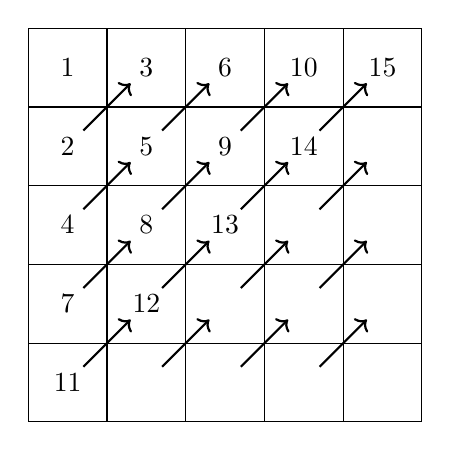
\begin{tikzpicture}[scale=1]
        % Grid
        \draw (0,0) grid (5,5);
        
        % Numbers specified (top-right triangle)
        \node at (0.5,4.5) {1};
        \node at (1.5,4.5) {3};
        \node at (2.5,4.5) {6};
        \node at (3.5,4.5) {10};
        \node at (4.5,4.5) {15};
        
        \node at (0.5,3.5) {2};
        \node at (1.5,3.5) {5};
        \node at (2.5,3.5) {9};
        \node at (3.5,3.5) {14};
        
        \node at (0.5,2.5) {4};
        \node at (1.5,2.5) {8};
        \node at (2.5,2.5) {13};
        
        \node at (0.5,1.5) {7};
        \node at (1.5,1.5) {12};
        
        \node at (0.5,0.5) {11};
        
        % Diagonal arrows
        \foreach \x in {0,...,3} {
            \foreach \y in {0,...,3} {
                \draw[->, thick] (\x+0.7,\y+0.7) -- (\x+1.3,\y+1.3);
            }
        }
      \end{tikzpicture}
      \caption{You can see that given $(x, y)$ it is on the $(x+y+1)$th diagonal, which starts from the $\frac{1}{2} \big((x+y+1)^2 - (x+y+1) + 2)$th number and increments by $x-1$. Therefore, we have the formula above. } 
      \label{fig:rationals_countable}
    \end{figure}
  \end{proof}

  \begin{theorem}[Finite Fields]
    There are no finite ordered fields. 
  \end{theorem} 
  \begin{proof}
    Assume $\mathbb{F}$ is such an ordered field. It must be the case that $0, 1 \in \mathbb{F}$, with $0 < 1$. Therefore, we also have $0 + 1 < 1 + 1 \implies 1 < 1 + 1$. Repeating this we get 
    \begin{equation}
      0 < 1 < 1 + 1 < 1 + 1 + 1 < \ldots
    \end{equation}
    where these elements must be distinct (since only one of $>, <, =$ must be true for a totally ordered set). Since this can be done for a countably infinite number of times, $\mathbb{F}$ cannot be finite. 
  \end{proof}

\subsubsection{Norm, Metric, and Topology on Rationals}

  Note that we can also define a norm on the rationals with just the order and algebraic properties. 

  \begin{theorem}[Norm on $\mathbb{Q}$] 
    The following is indeed a norm on $\mathbb{Q}$. 
    \begin{equation}
      |x| \coloneqq \begin{cases} x & \text{ if } x \geq 0 \\ -x & \text{ if } x < 0 \end{cases}
    \end{equation} 
  \end{theorem} 

  It is well known that the metric induced by any norm is indeed a metric. Therefore we state the metric as a definition. 

  \begin{definition}[Metric on $\mathbb{Q}$]
    The Euclidean metric on $\mathbb{Q}$ is defined 
    \begin{equation}
      d(x, y) \coloneqq |x - y| = \begin{cases} x - y & \text{ if } x \geq y \\ y - x & \text{ if } x < y \end{cases}
    \end{equation}
  \end{definition}

  Thus we get to what we want: the induced topology of open balls. 
  Again, since we know from point-set topology that metric topologies are indeed topologies, we will state this as a definition rather than a theorem.  

  \begin{definition}[Open-Ball Topology on $\mathbb{Q}$]
    The Euclidean topology on $\mathbb{Q}$ is the topology generated by the set $\mathscr{B}$ of all open balls
    \begin{equation}
      B(x, r) \coloneqq \{ y \in \mathbb{Q} \mid |x - y| < r \}
    \end{equation} 
  \end{definition}

  Note that this is the same topology as the order topology. This should however be proved. 

  \begin{theorem}[Metric and Order Topologies on $\mathbb{Q}$]
    The metric and order topologies on $\mathbb{Q}$ are the same topologies. 
  \end{theorem}
  \begin{proof}
    
  \end{proof}


\section{The Real Numbers}

  By constructing $\mathbb{Q}$ and its topology in my algebra and topology notes, we can talk about convergence. The first question to ask (if you were the first person inventing the reals) is ``how do I know that there exists some other numbers at all?'' The first clue is trying to find the side length of a square with area $2$. As we see, this number is not rational. 

  \begin{theorem}[$\sqrt{2}$ is Not Rational]
    \label{thm:sqrt2-irrational}
    There exists no $x \in \mathbb{Q}$ s.t. $x^2 = 2$. 
  \end{theorem}
  \begin{proof}
    Assume such a number $x = p/q$ exists, where $\mathrm{gcd}(p, q) = 1$. Then, by the field axioms of $\mathbb{Q}$, we can deduce that 
    \begin{equation}
      2 = \frac{p^2}{q^2} \implies 2 q^2 = p^2
    \end{equation}
    This implies that $2 \mid p$, so we have $p = 2p_0$, and we can write $2 q^2 = 4 p_0^2$. Dividing both sides by $2$, we get $q^2 = 2p_0^2$, which implies that $2 \mid q$. This contradicts the fact that $p$ and $q$ are coprime. 
  \end{proof} 

  We can ``imagine'' that a square with area $2$ certainly exists, but the fact that its side length is undefined is certainly unsettling. I don't know about you, but I would try to ``invent'' $\sqrt{2}$. We can do this in 4 distinct ways, though some may be more similar than others. 

  \begin{enumerate}
    \item \textit{Dedekind Completeness}. I would try and generate new elements by taking a specific \textit{cut}---a partition into two sets such that elements of one set is always greater than that of the other---and seeing which elements lie right in between these cuts. We will often see that we can always find a cut for every rational, but there are additional cuts for each irrational number. This is the idea behind \textit{Dedekind completeness}. 

    \item \textit{Cauchy Completeness}. I write out the decimal expansion one by one, which gives our first exposure to sequences. 
    \begin{equation}
      1, 1.4, 1.41, 1.414, \ldots
    \end{equation} 
    It is clear that on $\mathbb{Q}$, this sequence does not converge. Our intuition tells that that if the terms get closer and closer to each other, they must be getting closer and closer to \textit{something}, though that something is not in $\mathbb{Q}$. This motivates the definition for \textit{Cauchy completeness}. 

    \item \textit{Nested Interval Completeness}. I would write out maybe some nested intervals so that $\sqrt{2}$ \textit{must} lie within each interval. 
    \begin{equation}
      [1, 2] \supset [1.4, 1.5] \supset [1.41, 1.42] \supset \ldots 
    \end{equation}
    This motivates the definition of \textit{nested-interval completeness}. 

    \item \textit{Least Upper Bound Completeness}. I would define the set of all rationals such that $x^2 < 2$, and try to define $\sqrt{2}$ as the max or supremum of this set. We will quickly find that neither the max nor the supremum exists in $\mathbb{Q}$, and this motivates the definition for \textit{least upper bound completeness}. 
  \end{enumerate}

  All four of these methods points at the same intuition that there should not be any ``gaps'' or ``missing points'' in the set that we will construct to be $\mathbb{R}$, which is the general notion of \textit{completeness}. This contrasts with the rational numbers, whose corresponding number line has a "gap" at each irrational value. Even though constructing the reals with one method is sufficient, knowing the different flavors in which completeness manifests is very useful. It allows us to view properties of $\mathbb{R}$ through different lens. 

  The main division between these four properties is that the first two are methods to directly \textit{construct} the reals from $\mathbb{Q}$, while the latter two are more \textit{axiomatic properties} that we use to verify completeness for a given set. In the next two sections, we will take the rationals and add on extra elements using Dedekind cuts and Cauchy sequences. However, it isn't as conventional (though possible) to construct them as the single point contained in a sequence of nested intervals nor as a supremum of all upper-bounded sets. In fact, an alternative way to construct the reals is to define it axiomatically---as a totally ordered field with either the LUB property or the nested interval property.\footnote{In fact, you also need the Archimidean principle, but we'll talk about this later.} 

  Therefore, in the following sections, we will 
  \begin{enumerate}
    \item first define the relevant notion of completeness, 
    \item show that the rationals are not complete 
    \item and then construct the completed version of the rationals as a version of the reals. 
  \end{enumerate}
  Once we have done this for all three versions, we will unify them by proving they are all equivalent. 

  There is a second essential property of the reals that is not talked about as often is the Archimidean principle. 

  \begin{definition}[Archimidean Principle]
    An ordered ring $(X, +, \cdot, \leq)$ that embeds the naturals $\mathbb{N}$\footnote{as in, there exists an ordered ring homomorphism $\iota: \mathbb{N} \rightarrow X$} is said to obey the \textbf{Archimedean principle} if given any $x, y \in X$ s.t. $x, y > 0$, there exists an $n \in \mathbb{N}$ s.t. $\iota(n) \cdot x > y$. Usually, we don't care about the canonical injection and write $nx > y$. 
  \end{definition} 
  
  \begin{lemma}[Rationals are Archimidean]
    $\mathbb{Q}$ satisfies the Archimidean principle. 
  \end{lemma}
  \begin{proof}
    Take any $x = p_1/q_1, y = p_2 / q_2 \in \mathbb{Q}$. Then, take $n = q_1 p_2$, and we get 
    \begin{equation}
      n x = q_1 p_2 \frac{p_1}{q_1} = p_1 p_2 > \frac{p_2}{q_2} = y \iff p_1 > \frac{1}{q_2}
    \end{equation}
    which must be true since $p_1 \geq 1 \geq \frac{1}{q_2}$. 
  \end{proof}

  Usually, we just construct $\mathbb{R}$ right out of $\mathbb{Q}$, and it turns out that the Archimidean principle just trivially follows. However, if we construct $\mathbb{R}$ axiomatically (without the rationals), it needs to be stated. In this axiomatic formulation, we will find that certain types of completeness---like Dedekind completeness---actually \textit{implies} the Archimidean principle, while others---like Cauchy and nested-intervals completeness---does not. Therefore, in a sense, Dedekind completeness is the ``strongest'' form of completeness. 

\subsection{Dedekind Completeness}  

  This is an explicit construction from the rationals. 

  \begin{definition}[Dedekind Cut] 
    A \textbf{Dedekind cut} is a partition of the rationals $\mathbb{Q} = A \sqcup A^\prime$ satisfying the three properties.\footnote{This can really be defined for any totally ordered set. } 
    \begin{enumerate}
      \item $A \neq \emptyset$ and $A \neq \mathbb{Q}$.\footnote{By relaxing this property, we can actually complete $\mathbb{Q}$ to the extended real number line. }
      \item $x < y$ for all $x \in A, y \in A^\prime$. 
      \item The maximum element of $A$ does not exist in $\mathbb{Q}$. 
    \end{enumerate}
    The minimum of $A^\prime$ may exist in $\mathbb{Q}$, and if it does, the cut is said to be \textbf{generated} by $\min A^\prime$. 
  \end{definition}

  Note that in $\mathbb{Q}$, there will be two types of cuts: 
  \begin{enumerate}
    \item ones that are generated by rational numbers, such as 
    \begin{equation}
      A = \{x \in \mathbb{Q} \mid x < 2/3 \}, A^\prime = \{ x \in \mathbb{Q} \mid x \geq 2/3 \} 
    \end{equation}
    \item and the ones that are not 
    \begin{equation}
      A = \{x \in \mathbb{Q} \mid x^2 < 2 \}, A^\prime = \{x \in \mathbb{Q} \mid x^2 \geq 2 \}
    \end{equation}
  \end{enumerate}
  We can intuitively see that the set of all Dedekind cuts $(A, A^\prime)$ will ``extend'' the rationals into a bigger set. We can then define some operations and an order to construct this into an ordered field, and finally it will have the property that we call ``completeness.''

  \begin{definition}[Dedekind Completeness]
    A totally ordered algebraic field $\mathbb{F}$ is \textbf{Dedekind-complete} if every Dedekind cut of $\mathbb{F}$ is generated by an element of $\mathbb{F}$. 
  \end{definition}

  \begin{lemma}[Rationals are Not Dedekind-Complete]
    $\mathbb{Q}$ is not Dedekind-complete. 
  \end{lemma}
  \begin{proof}
    Take a look at the cut
    \begin{equation}
      A = \{x \in \mathbb{Q} \mid x^2 < 2 \}, A^\prime = \{x \in \mathbb{Q} \mid x^2 \geq 2 \}
    \end{equation}
    We wish to show that $A^\prime$ has no minimum. Assume that it does, and call it $p$. Then, define 
    \begin{equation}
      q \coloneqq p - \frac{p^2 - 2}{p + 2} = \frac{2p + 2}{p + 2} 
    \end{equation}
    We can see that $p > 2 \implies p^2 - 2 > 0 \implies q < p$. But we also see that 
    \begin{equation}
      q^2 - 2 = \frac{2 (p^2 - 2)}{(p + 2)^2} \implies q^2 > 2
    \end{equation}
    Therefore, we have found a $q \in A^\prime$ that is smaller than $p$, a contradiction. 
  \end{proof}

  These Dedekind cuts are simply subsets of the power set of $\mathbb{Q}$, which always exists due to the \hyperref[st-power-set-axiom]{power set axiom}. Therefore, we can simply use the axiom of restricted comprehension (?) to create a well-defined set of Dedekind cuts.    

  \begin{definition}[Reals as the Dedekind-Completion of Rationals]
    Let $\mathbb{R}_D$ be the set of all Dedekind cuts $A$\footnote{For convenience we can uniquely represent $(A, A^\prime)$ with just $A$ since $A^\prime = \mathbb{Q} \setminus A$. }  of $\mathbb{Q}$. 

    \begin{equation}
      \mathbb{R}_D \coloneqq \{ A \in 2^{\mathbb{Q}} \mid (A, A^c) \text{ is a Dedekind cut}\}
    \end{equation}
    By doing this we can intuitively think of a real number as being represented by the set of all smaller rational numbers. Let $A, B \in \mathbb{R}_D$ two Dedekind cuts. Then, we define the following order and operations. 
    \begin{enumerate}
      \item \textit{Order}. $A \leq_{\mathbb{R}} B \iff A \subset B$. 
      \item \textit{Addition}. $A +_{\mathbb{R}} B \coloneqq \{ a +_{\mathbb{Q}} b \mid a \in A, b \in B \}$. 
      \item \textit{Additive Identity}. $0_{\mathbb{R}} \coloneqq \{x \in \mathbb{Q} \mid x < 0 \}$. 
      \item \textit{Additive Inverse}. $-B \coloneqq \{ a - b \mid a < 0 , b \in (\mathbb{Q} \setminus B) \}$.
      \item \textit{Multiplication}. If $A, B \geq 0$, then we define $A \times_{\mathbb{R}} B \coloneqq \{ a \times_{\mathbb{Q}} b \mid a \in A, b \in B, a, b \geq 0\} \cup 0_{\mathbb{R}}$. If $A$ or $B$ is negative, then we use the identity $A \times B = -(A \times_{\mathbb{R}} -B) = -(-A \times_{\mathbb{R}} B) = (-A \times_{\mathbb{R}} -B)$ to convert $A, B$ to both positives and apply the previous definition. 
      \item \textit{Multiplicative Identity}. $1_{\mathbb{R}} = \{x \in \mathbb{Q} \mid x < 1 \}$. 
      \item \textit{Multiplicative Inverse}. If $B > 0$, $B^{-1} \coloneqq \{ a \times_{\mathbb{Q}} b^{-1} \mid a \in 1_{\mathbb{R}}, b \in (\mathbb{Q} \setminus B) \}$. If $B$ is negative, then we compute $B^{-1} = -((-B)^{-1})$ by first converting to a positive number and then applying the definition above. 
    \end{enumerate}

    We claim that $(\mathbb{R}, +_{\mathbb{R}}, \times_{\mathbb{R}}, \leq_{\mathbb{R}})$ is a Dedekind-complete totally ordered field, and the canonical injection $\iota: \mathbb{Q} \rightarrow \mathbb{R}$ defined 
    \begin{equation}
      \iota(q) = \{x \in \mathbb{Q} \mid x < q \}
    \end{equation}
    is an ordered field isomorphism. 
  \end{definition} 
  \begin{proof}
    
  \end{proof}

  By the canonical injections $\mathbb{N} \rightarrow \mathbb{Z} \rightarrow \mathbb{Q} \rightarrow \mathbb{R}_D$, we can talk about whether this set has the Archimedean property. By construction, Archimidean is trivial since $\mathbb{R}_D$ contains $\mathbb{Q}$ which is Archimidean. 

  \begin{theorem}[Dedekind Reals is Archimedean]
    $\mathbb{R}_D$ satisfies the Archimedean principle. 
  \end{theorem}
  \begin{proof} 
    $\mathbb{R}_D$ contains $\mathbb{Q}$. 
  \end{proof}

  \begin{definition}[Axiomatic Construction of Dedekind-Reals]
    $\mathbb{R}_D^\prime$ is a totally ordered field that is Dedekind complete.\footnote{Just for this section, I will denote $\mathbb{R}^\prime$ as reals constructed axiomatically.}
  \end{definition}

  \begin{theorem}[Axiomatic Dedekind Reals is Archimedean]
    $\mathbb{R}_D^\prime$ satisfies the Archimedean principle. 
  \end{theorem}
  \begin{proof}
    Assume that this property doesn't hold. Then for any fixed $x$, $nx < y$ for all $n \in \mathbb{N}$. Consider the set 
    \begin{equation}
      A = \bigcup_{n \in \mathbb{N}} (-\infty, nx), \qquad B = \mathbb{R} \setminus A
    \end{equation}
    $A$ by definition is nonempty, and $B$ is nonempty since it contains $y$. Then, we can show that $a \in A, b \in B \implies a < b$ using proof by contradiction. Assume that there exists $a^\prime \in A, b^\prime \in B$ s.t. $a^\prime > b^\prime$. Since $a^\prime \in A$, there exists a $n^\prime \in \mathbb{N}$ s.t. $a^\prime \in (-\infty, n^\prime x) \iff a^\prime < n^\prime x$. But by transitivity of order, this means $b^\prime < n^\prime x \iff b^\prime \in (-\infty, n^\prime x) \implies b^\prime \in A$. 

    Going back to the main proof, we see that $A$ is upper bounded by $y$, and so by the least upper bound property it has a supremum $z = \sup{A}$. 
    \begin{enumerate}
      \item If $z \in A$, then by the induction principle\footnote{Note that $\mathbb{N}$ is defined recursively as $1 \in \mathbb{N}$ and if $n \in \mathbb{N}$, then $n+1 \in \mathbb{N}$. } $z + x \in A$, contradicting that $z$ is an upper bound. 
      \item If $z \not\in A$, then by the induction principle\footnote{The contrapositive of the recursive definition of $\mathbb{N}$ is: if $n \not\in \mathbb{N}$, then $n-1 \not\in \mathbb{N}$.} $z-x \not\in A \implies z-x \in B$. Since every element of $B$ upper bounds $A$ and since $x > 0$, this means that $z-x < z$ is a smaller upper bound of $A$, contradicting that $z$ is a least upper bound. 
    \end{enumerate}
    Therefore, it must be the case that $nx > y$ for some $n \in \mathbb{N}$. 
  \end{proof}

\subsection{Cauchy Completeness} 

  In many cases we are not working with ordered fields, and so different types of completeness may be more useful. In actual practice, you tend to use Cauchy completeness which only assumes a metric structure. 

  \begin{definition}[Cauchy Sequence]
    A sequence $(x_n)_n$ in a metric space $(X, d)$ is a \textbf{Cauchy sequence} if $\forall \epsilon > 0$, $\exists N \in \mathbb{N}$ s.t.  
    \begin{equation}
      n, m \geq N \implies d(x_n, x_m) < \epsilon
    \end{equation}
  \end{definition}

  To motivate this definition, note that in a general topological space $X$, we can define convergence of a sequence $x_n \to x$ perfectly fine. However, take some subset $U \subset X$, and let $x$ be a limit point of $U$. In this case, $x_n$ does not converge in $U$, but it does converge to something outside of $U$---namely, $x \in X$. This is similar to $\mathbb{Q} \subset \mathbb{R}$, where $x$ is an irrational point. However, we are trying to \textit{construct} $\mathbb{R}$, so Cauchy convergence allows us to speak of convergence without actually referring to \textit{what} a sequence is converging to. 

  Note that it is not sufficient to say that a sequence is Cauchy by claiming that each term becomes arbitrarily close to the preceding term. That is, 
  \begin{equation}
    \lim_{n \rightarrow \infty} d(x_{n+1}, x_{n}) = 0
  \end{equation}

  \begin{example}[Adjacent Terms Converging Doesn't Imply Sequence is Cauchy]
    For example, look at the sequence 
    \begin{equation}
      a_n = \sqrt{n} \implies a_{n+1} - a_{n} = \frac{1}{\sqrt{n+1} + \sqrt{n}} < \frac{1}{2\sqrt{n}}
    \end{equation}
    However, it is clear that $a_n$ gets arbitrarily large, meaning that a finite interval can contain at most a finite number of terms in $\{a_n\}$. 
  \end{example}

  It is often more convenient to think of the limit of the \textit{diameter} of rest of the sequence. That is, a sequence is Cauchy if 
  \begin{equation}
    \lim_{n \rightarrow \infty} \mathrm{diam}\{x_{m}\}_{m \geq n} = 0
  \end{equation}

  It is trivial that convergence implies Cauchy convergence, but the other direction is not true. Therefore, we would like to work in a space where these two are equivalent, and this is called completeness. Therefore, we can construct the reals as equivalence classes over Cauchy sequences. Rather than using the order, we take advantage of the metric. 

  \begin{definition}[Cauchy Completeness]
    A metric space $(X, d)$ is \textbf{Cauchy complete} if every Cauchy sequence in that space converges to an element in $X$. 
  \end{definition} 
  
  $\mathbb{Q}$ is not Cauchy-complete. Let $a_n$ be the largest number $x$ up to the $n$th decimal expansion such that $x^2$ does not exceed $2$. The first few terms are 
  \begin{equation}
    1.4, 1.41, 1.414, \ldots
  \end{equation}
  In this case, we can see that this is Cauchy since at the $n$th element and on, the first $n$ decimal places are kept fixed and so the most that the rest of the sequence can deviate by is $10^{-n}$. 

  \begin{definition}[Reals as the Cauchy-Completion of the Rationals]
    Let $\mathbb{R}_C$ be the quotient space of all Cauchy (under the Euclidean metric) sequences $(x_n)$ of rational numbers with the equivalence relation $(x_n) = (y_n)$ iff their difference tends to $0$.\footnote{This equivalence class reflects that the same real number can be approximated in many different sequences. In fact, this shows \textit{by definition} that $1, 1, \ldots$ and $0.9, 0.99, 0.999, \ldots$ are the same number!} That is, for every rational $\epsilon > 0$, there exists an integer $N$ s.t. for all naturals $n > N$, $|x_n - y_n| < \epsilon$. 
    \begin{enumerate}
      \item \textit{Order}. $(x_n) \leq_{\mathbb{R}} (y_n)$ iff $x = y$ or there exists $N \in \mathbb{N}$ s.t. $x_n \leq_{\mathbb{Q}} y_n$ for all $n > N$. 
      \item \textit{Addition}. $(x_n) + (y_n) \coloneqq (x_n + y_n)$. 
      \item \textit{Additive Identity}. $0_{\mathbb{R}} \coloneqq (0_{\mathbb{Q}})$. 
      \item \textit{Additive Inverse}. $-(x_n) \coloneqq (-x_n)$. 
      \item \textit{Multiplication}. $(x_n) \times_{\mathbb{R}} (y_n) = (x_n \times_{\mathbb{Q}} y_n)$. 
      \item \textit{Multiplicative Identity}. $1_{\mathbb{R}} \coloneqq (1)$. 
      \item \textit{Multiplicative Inverse}. $(x_n)^{-1} \coloneqq (x_n^{-1})$. 
    \end{enumerate}
    We claim that $(\mathbb{R}, +_{\mathbb{R}}, \times_{\mathbb{R}}, \leq_{\mathbb{R}})$ is a totally ordered field, and the canonical injection $\iota: \mathbb{Q} \rightarrow \mathbb{R}$ defined 
    \begin{equation}
      \iota(q) = (q)
    \end{equation} 
    is an ordered field isomorphism. Finally, by construction $\mathbb{R}$ is Cauchy-complete. 
  \end{definition}
  \begin{proof}
    
  \end{proof}

  \begin{theorem}[Cauchy Reals is Archimidean]
    $\mathbb{R}_C$ satisfies the Archimedean principle. 
  \end{theorem}
  \begin{proof}
    $\mathbb{R}_C$ contains $\mathbb{Q}$, which is Archimidean. 
  \end{proof}

  The best thing about Cauchy completeness is that we can just take $\mathbb{Q}^n$ to create $\mathbb{R}^n$. It becomes quite general. However, note that first, Cauchy completion depends on \textit{which} metric you use to complete it. 

  \begin{example}[P-adic Numbers]
    Let $p$ be a prime number. For a non-zero rational $x = p^k \cdot \frac{a}{b}$ where $p \nmid a, b$, define the \textbf{p-adic norm}\footnote{This measures divisibility by $p$: the more $p$ divides $x$, the smaller $|x|_p$. For example, $|8|_2 = 2^{-3} = 1/8$ and $|3|_2 = 1$.} as 
    \begin{equation}
      |x|_p \coloneqq p^{-k}, \qquad |0|_p \coloneqq 0
    \end{equation}
    The \textbf{p-adic numbers} $\mathbb{Q}_p$ are the Cauchy completion of $\mathbb{Q}$ with respect to the p-adic metric $d_p(x,y) = |x - y|_p$. This set not only does not satisfy the Archimidean principle; it doesn't even have a natural ordering! 
  \end{example} 

  \begin{definition}[Axiomatic Construction of Cauchy-Reals]
    $\mathbb{R}_D^\prime$ is a totally ordered field that is Cauchy complete and that satisfies the Archimidean principle.
  \end{definition}

  Note that we require the extra Archimidean assumption in the axiomatic construction. 

  \begin{example}[Ordered Cauchy-Complete Fields that are Not Archimidean]
    Provide examples of ordered, Cauchy-complete fields that are not Archimedean. Hyperreals? 
  \end{example}

\subsection{Least Upper Bound Completeness}

  \begin{definition}[Least Upper Bound Property]
    A totally ordered algebraic field $\mathbb{F}$ (must it be a field?) is \textbf{least-upper-bound complete}, or is said to satisfy the \textbf{least upper bound (LUB) property}, if every nonempty set of $\mathbb{F}$ having an upper bound must have a least upper bound (supremum) in $\mathbb{F}$. 
  \end{definition} 

  \begin{theorem}[LUB is Equivalent to GLB]
    A set $(\mathbb{F}, \leq)$ has the least upper bound property iff it has the \textit{greatest lower bound property}, which states that every set bounded below has a greatest lower bound. 
  \end{theorem}
  \begin{proof}
    We will prove one direction since the other is the same logic. Let $S \subset X$ be a nonempty set that is bounded below by some $l \in X$. Let $L \subset X$ be the set of all lower bounds of $S$. Since $l$ exists, it is nonempty. Furthermore, $L$ is bounded above by any element of $S$. Due to LUB property $L$ has a least upper bound, call it $z = \sup{L}$. We claim that $z = \inf{S}$. 
    \begin{enumerate}
      \item $z$ is a lower bound of $S$. Assume that it is not. Then there exists $s \in S$ s.t. $s < z$. But by construction $s$ is an upper bound for $L$ and so $z$ s not the \textit{least} upper bound, a contradiction. 
      \item $z$ is a \textit{greatest} lower bound. Assume that $z$ is not. Then there exists a $z^\prime \in X$ s.t. $z < z^\prime \leq s$ for all $s \in S$. But since $z^\prime, z$ are lower bounds, this means $z, z^\prime \in L$ by definition and $z < z^\prime$ contradicts the fact that $z$ is an upper bound of $L$. 
    \end{enumerate}
    We are done. 
  \end{proof}

  $\mathbb{Q}$ does not satisfy the least upper bound property, but proving this can be tricky for the first time. We state this as a lemma. 

  \begin{theorem}[Rationals Doesn't Satisfy LUB Property]
    $\mathbb{Q}$ does not satisfy the LUB property. 
  \end{theorem}
  \begin{proof}
    Assume it does, and let us denote 
    \begin{equation}
      p \coloneqq \sup \{x \mid \mathbb{Q} \mid x^2 < 2\} \in \mathbb{Q}
    \end{equation}
    The key here is to find another rational that we can always ``squeeze'' in between $p$ and $2$. This can be done with the Archimidean principle, which is already satsified in $\mathbb{Q}$. Since we have \href{thm:sqrt2-irrational}{proved that there exists no rational that squares to $2$}, we only need to consider the two cases. 
    \begin{enumerate}
      \item $p^2 < 2$. Take $\epsilon \in \mathbb{Q}$ so small that 
      \begin{equation}
        p^2 + 2 p \epsilon + \epsilon^2 = (p + \epsilon)^2 < 2
      \end{equation}
      To show complete steps, we can see that by density of reals, there exists some rational $r$ s.t. $0 < r < 2 - p^2$. Therefore, we can invoke Archimidean principle to find a $n \in \mathbb{N}$ s.t. $\epsilon = p/n < 2 p/n < r$. Therefore, $p$ is not an upper bound, so this cannot be true. 

      \item $p^2 > 2$. We can again take an $\epsilon \in \mathbb{Q}$ so small that 
      \begin{equation}
        p^2 - 2 p \epsilon + \epsilon^2 = (p - \epsilon)^2 > 2
      \end{equation}
      Therefore, $p$ is not least, so this cannot be true. 
    \end{enumerate}
  \end{proof}

  \begin{definition}[Axiomatic Construction of Reals with LUB Property]
    $\mathbb{R}_I^\prime$ is a totally ordered field that satisfies the least upper bound property.
  \end{definition}

  Note that we don't need to explicitly assume Archimidean principle here. The LUB property is strong enough that it implies Archimidean!

  \begin{theorem}[LUB Property Implies Archimidean]
    $\mathbb{R}_I^\prime$ is Archimidean. 
  \end{theorem}

  Now let's see how our previous constructions of the reals relate to the LUB property. 

  \begin{theorem}[Dedekind Completed Reals Satisfies LUB Property]
    $\mathbb{R}_D$ satisfies the least upper bound property. 
  \end{theorem}
  \begin{proof}
    Let $\mathcal{A}$ be a nonempty subset of $\mathbb{R}_D$ bounded from above by $T$. Then, $\forall A \in \mathcal{A}$, $A \coloneqq (A, A^c)$ is a Dedekind cut, and we can define
    \begin{equation}
      (B, B^\prime) \coloneqq \bigg( \bigcup_{A \in \mathcal{A}} A, \bigcap_{A \in \mathcal{A}} A^c \bigg)
    \end{equation} 
    We claim that this is a Dedekind cut. 
    \begin{enumerate}
      \item First, it is nonempty set $\mathcal{A} \neq \emptyset$ and so for each $A \in \mathcal{A}$, $A \subset \mathbb{Q}$ is nonempty. It is also not all of $\mathbb{Q}$ since $T$ is an upper bound of $\mathcal{A}$, and so $T \geq a \; \forall a \in A \; \forall A \in \mathcal{A}$, which implies that 
      \begin{equation}
        T \not\in \bigcup_{A \in \mathcal{A}} A
      \end{equation}

      \item Now let $x \in B, y \in B^\prime$. Then, $x \in A_0$ for some $A_0 \in \mathcal{A}$, and since $y$ is in the intersection of all the corresponding $A^c$, it must be in the corresponding $A_0^c$. Therefore we invoke the Dedekind cut property of $(A_0, A_0^c)$ and see $x < y$. 

      \item Finally, for the sake of contradiction, let $m \in \mathbb{Q}$ be the maximum of $B$. Then, $m \in A^\ast$ for some $A^\ast \in \mathcal{A}$. But $m$ is an upper bound for the whole $B$, so this means that $m = \max\{A^\ast\}$, which contradicts the fact that lower cut cannot have a rational maximum. 
    \end{enumerate}
    Now we claim that $B$ is the supremum. It is an upper bound since 
    \begin{equation}
      A \subset B = \bigcup_{A \in \mathcal{A}} A \quad \forall A \in \mathcal{A}
    \end{equation}
    To prove least, we should see that if $(S, S^c)$ is another upper bound of $\mathcal{A}$, then $A \subset S$ for all $A \in \mathcal{A} \implies B = \bigcup_{A \in \mathcal{A}} A \subset S$, which establishes that $B$ is least. 
  \end{proof}

\subsection{Nested Intervals Completeness}

  The next flavor we present is nested-intervals completeness.  This is the least popular way to construct the reals, and it is used more as a post-hoc tool to analyze the reals after you construct it using either of the two previous methods. 

  \begin{definition}[Nested Interval Completeness]
    Let $\mathbb{F}$ be a totally ordered algebraic field. Let $I_n= [a_n, b_n]$ ($a_n < b_n$) be a sequence of decreasing nested intervals that are 
    \begin{enumerate}
      \item closed, 
      \item bounded, 
      \item nested, $I_1 \supset I_2 \supset I_3 \supset \ldots$ 
      \item and decreasing to $0$ in the sense that $\lim_{n \to \infty} b_n - a_n = 0$. 
    \end{enumerate}
    $\mathbb{F}$ is \textbf{nested-interval complete} if the intersection of all of these intervals $I_n$ contains exactly one point. 
    \begin{equation}
      \bigcup_{n=1}^\infty I_n \in \mathbb{F}
    \end{equation}
  \end{definition}

  Note that defining nested intervals requires only an ordered field. One may look at this and try to ask if this is a specific instance of the following conjecture: The intersection of a nested sequence of nonempty closed sets in a topological space has exactly 1 point. This claim may not even make sense, actually. If we define nested in terms of proper subsets, then for a finite topological space a sequence cannot exist since we will run out of open sets and so this claim is vacuously true and false. If we allow $S_n = S_{n+1}$ then we can just select $X \supset X \supset \ldots$, which is obviously not true. However, a slightly weaker claim is that every proper nested non-empty closed sets has a non-empty intersection is a consequence of compactness. 

  \begin{theorem}[Rationals are Not Nested-Interval Complete]
    $\mathbb{Q}$ is not nested-interval complete. 
  \end{theorem}
  \begin{proof}
    This is a nice proof that uses a class method of algorithmically selecting nested intervals that satisfy a following property. This trick will be used many times in analysis. 
    
    For the sake of contradiction, let us assume that $\mathbb{Q}$ satisfies nested intervals completeness. Since $\mathbb{Q}$ is countable, enumerate it as $q_1, q_2, \ldots$. 
    \begin{enumerate}
      \item Choose any closed interval $I_1$ of length $1$ with rational endpoints that doesn't contain $q_1$. 
      \item Now partition $I_1$ into two segments of equal length, and choose $I_2$ to be the segment that doesn't contain $q_2$.  
    \end{enumerate}
    At this point, $I_n$ is a closed interval with rational endpoints of length $2^{-n}$ that cannot contain $q_n$. Therefore, $\cap_n I_n$ cannot contain any $q_n \in \mathbb{Q}$. But this contradicts our assumption of nested interval completeness.  
  \end{proof} 

  One may ask: what is the relationship between LUB property and nested-intervals completeness? It turns out that they are equivalent. 

  \begin{theorem}[LUB is Equivalent to Nested Interval Completeness in Reals]
    Listed. 
    \begin{enumerate}
      \item $\mathbb{R}_L^\prime$ satisfies nested intervals completeness. 
      \item $\mathbb{R}_I^\prime$ satisfies least upper bound completeness. 
    \end{enumerate}
  \end{theorem}
  \begin{proof}
    Listed. 
    \begin{enumerate}
      \item Note that $\{a_n\}$ is bounded above by $b_1$. Therefore by LUB property it must have a supremum, call it $x = \sup_n \{a_n\}$. Then, we see that $a_n \leq x \leq b_n$ for all $n$, and so $x$ is in the intersection. 
    \end{enumerate}
  \end{proof}

  \begin{theorem}[Cantor's Intersection Theorem]
    $\mathbb{R}$ is nested-interval complete. 
  \end{theorem}
  \begin{proof}
    We prove this by first proving the claim that given nested, closed, and bounded sets $I_n$ (not even necessarily intervals), then 
    \begin{equation}
      \bigcap_{n=1}^\infty I_n \neq \emptyset
    \end{equation}
    Suppose this is not true. For every $x \in \mathbb{R}$, there exists a $n_x$ s.t. $x \not\in I_n$ (and all later $I_m$ for $m > n$). Let $O_n = I_n^c$ open sets. Then, $\mathbb{R} \subset \cup_n O_n$ In particular, $I_1 \subset \cup_n O_n$. But $I_1$ is closed and bounded. So we can extract a finite subcover. $O_{n_1}, O_{n_2}, \ldots, O_{n_m}$ (ordered $n_1 < n_2 < \ldots< n_m$). Then since $O_n$ are increasing, $I_1 \subset O_{n_m} = I_{n_m}^c$. But $I_{n_m} \subset I_1$, a contradiction. 

    Now with this, we know that because the limits of the endpoints of the intervals go to $0$, then there cannot be more than 2 points in the intersection. Thus there must be 1 unique point. 
  \end{proof} 

  \begin{definition}[Axiomatic Construction of Reals with Nested Intervals]
    $\mathbb{R}_I$ is a totally ordered field that 
    \begin{enumerate}
      \item satisfies the nested intervals completeness, and 
      \item satisfies the Archimidean principle.
    \end{enumerate}
  \end{definition}

\subsection{Properties of the Real Line}  

  Perfect, now all that remains is to unite the two constructions of the reals. 

  \begin{theorem}[Dedekind and Cauchy Complete Reals are Isomorphic]
    Given that $\mathbb{R}_D$ is the Dedekind-completed version of the rationals and $\mathbb{R}_C$ is the Cauchy-completed version of the rationals, we claim that the two are isomorphic as ordered fields. 
    \begin{equation}
      \mathbb{R}_D \simeq \mathbb{R}_C
    \end{equation}
  \end{theorem}
  \begin{proof}
    
  \end{proof}

  Therefore, it doesn't really matter which one we talk about, and we can refer to \textit{the} real numbers as a single set. Great! Now we can finally feel satisfied about defining metrics, norms, and inner products as mappings to the codomain $\mathbb{R}$. 

  \begin{definition}[Reals (as Construction from Rationals)]
    The \textbf{reals} $\mathbb{R}$ is the totally ordered complete Archimedean field constructed as the completion\footnote{either one} of $\mathbb{Q}$. 
  \end{definition}

  So far, we have taken the completion of the rationals as our main mode of construction. However, we can take an axiomatic approach, and it turns out that there is only one set, up to isomorphism, that satisfies all these properties. 

  \begin{theorem}[Axiomatic Definition of Reals]
    The \textbf{real numbers}, denoted $\mathbb{R}$, is any totally ordered complete Archimedean field. $\mathbb{R}$ is unique up to field isomorphism. That is, if two individuals construct two ordered complete Archimedean fields $\mathbb{R}_A$ and $\mathbb{R}_B$, then 
    \begin{equation}
      \mathbb{R}_A \simeq \mathbb{R}_B
    \end{equation}
  \end{theorem} 
  \begin{proof}
    The proof is actually much longer than I expected, so I draw a general outline.\footnote{Followed from \href{https://math.ucr.edu/~res/math205A/uniqreals.pdf}{here}.} We want to show how to construct an isomorphism $f: \mathbb{R}_A \rightarrow \mathbb{R}_B$. 
    \begin{enumerate}
      \item Realize that there are unique embeddings of $\mathbb{N}$ in $\mathbb{R}_A$ and $\mathbb{R}_B$ that preserve the inductive principle, the order, closure of addition, and closure of multiplication, the additive identity, and the multiplicative identity. Call these ordered doubly-monoid (since it's a monoid w.r.t. $+$ and $\times$) homomorphisms $\iota_A, \iota_B$. 
      \item Construct an isomorphism $f_1: \iota_A(\mathbb{N}) \rightarrow \iota_B(\mathbb{N})$ that preserves the inductive principle, order, addition, and multiplication. This is easy to do by just constructing $f_1 = \iota_B \circ \iota_A^{-1}$. 
      \item Extend $f_1$ to the ordered ring isomorphism $f_2$ by explicitly defining what it means to map additive inverses, i.e. negative numbers. 
      \item Extend $f_2$ to the ordered field isomorphism $f_3$ by explicitly defining what it means to map multiplicative inverses, i.e. reciprocals. 
      \item Extend $f_3$ to the ordered field isomorphism on the entire domain $\mathbb{R}_A$ and codomain $\mathbb{R}_B$. There is no additional operations that we need to support, but we should explicitly show that this is both injective and surjective, which completes our proof. 
    \end{enumerate}
  \end{proof}

  It seems that the real numbers is \textit{any} set that satisfies the definition above. Therefore, a line $\mathbb{L}$ with $+$ associated with the translation of $\mathbb{L}$ along itself and $\cdot$ associated with the "stretching/compressing" of the line around the additive origin $0$ is a valid representation of the reals. $\mathbb{R}$ can also be represented as an uncountable list of numbers with possibly infinite decimal points, known as the decimal number system. 
  \begin{equation}
    \ldots, -2.583\ldots, \ldots , 0, \ldots, 1.2343\ldots, \ldots, \sqrt{2}, \ldots
  \end{equation}

  The first property we should know is that the reals are uncountable. 

  \begin{theorem}[Cantor's Diagonalization]
    $\mathbb{R}$ is uncountable.
  \end{theorem}
  \begin{proof}
    We proceed by contradiction. Suppose the real numbers are countable. Then there exists a bijection $f: \mathbb{N} \to \mathbb{R}$. This means we can list all real numbers in $[0,1]$ as an infinite sequence.\footnote{This must be explicitly proven, but we can take the set of all Cauchy sequences of rationals in their decimal expansion and construct the reals this way.}
    
    \begin{align}
      f(1) &= 0.a_{11}a_{12}a_{13}\dots \\
      f(2) &= 0.a_{21}a_{22}a_{23}\dots \\
      f(3) &= 0.a_{31}a_{32}a_{33}\dots \\
      &\vdots
    \end{align}
    
    where each $a_{ij}$ is a digit between 0 and 9.
    
    Now construct a new real number $r = 0.r_1r_2r_3\dots$ where:
    \begin{equation}
      r_n = \begin{cases}
        1 & \text{if } a_{nn} \neq 1 \\
        2 & \text{if } a_{nn} = 1
      \end{cases}
    \end{equation}
    This number $r$ is different from $f(n)$ for every $n \in \mathbb{N}$, since $r$ differs from $f(n)$ in the $n$th decimal place. Therefore $r \in [0,1]$ but $r \notin \text{range}(f)$, contradicting that $f$ is surjective. Thus our assumption that the real numbers are countable must be false.
  \end{proof}

  With this, we can add the inner product, metric, and topology. 

\subsection{Exponentials, Roots, and Logarithms} 

  Now we will focus on some other operations that become well-defined in the reals. We know that $x^{n}$ for $n \in \mathbb{N}$ denotes repeated multiplication and $x^{-1}$ denotes the multiplicative inverse. We need to build up on this notation. As a general outline, we will show that $x^{-n}$ is well defined, then $x^q, q \in \mathbb{Q}$ is well-defined, and finally $x^r, r \in \mathbb{R}$ is well-defined. For the naturals, we have defined $x^n$ as the repeated multiplication of $n$. It is trivial that the canonical injection $\iota_0: \mathbb{N} \rightarrow \mathbb{R}$ commutes with the exponential map of naturals. We prove that $\iota_1: \mathbb{Z} \rightarrow \mathbb{R}$ also commutes. 

  \begin{lemma}[Integer Exponents]
    We have 
    \begin{enumerate}
      \item For $x_1, \ldots, x_n \in \mathbb{R}$, $(x_1 \ldots x_n)^{-1} = x_n^{-1} \ldots x_1^{-1}$. 
      \item For $x \in \mathbb{R}$, $x > 0$, $(x^n)^{-1} = (x^{-1})^n$. This value is denoted $x^{-n}$. 
      \item For $x \in \mathbb{R}$ and $w, z \in \mathbb{Z}$, $x^{w + z} = x^w x^z$. 
      \item For $w, z \in \mathbb{Z}$, $x^{wz} = (x^z)^w = (x^w)^z$. 
    \end{enumerate}
  \end{lemma}
  \begin{proof}
    Listed. 
    \begin{enumerate}
      \item The proof is trivial, but for $n = 2$ and $x_1 = x, x_2 = y$, we see that by associativity, $(x^{-1} x^{-1}) (x y) = y^{-1} (x^{-1} x) y = y^{-1} y = 1$ and we know inverses are unique. 
      \item Set $x_i = x$ using (1). 
      \item If $w, z > 0$ this is trivial by the associative property. If either or both are negative, say $w < 0 < z$, then we set $w^\prime = -w > 0$ and using (2) we know that 
      \begin{equation}
        x^{w} x^{z} = (x^{-1})^{w^\prime} x^z = x^{-w^\prime + z} = x^{w + z}
      \end{equation}
      by associativity in the second last equality. 
    \end{enumerate}
  \end{proof}

  Therefore, we have successfully defined $x^z$ for all $z \in \mathbb{Z}$, and if $z$ is negative, we're allowed to ``swap'' the $-1$ and $|z|$ in the exponents. Now we want to extend this into rational exponents, first by proving the existence and uniqueness of $n$th roots for any real. The proof is a little involved, but the general idea is that we want to use the LUB property to define the $n$th root as the supremum of a set.  

  \begin{theorem}[Existence of Nth Roots]
    For any real $x > 0$ and every $n \in \mathbb{N}$ there is one and only one positive real $y \in \mathbb{R}$ s.t. $y^n = x$. This is denoted $x^{1/n}$. 
  \end{theorem}
  \begin{proof}
    Let $E$ be the set consisting of all reals $t \in \mathbb{R}$ s.t. $t^n < x$. We show that 
    \begin{enumerate}
      \item it is nonempty. Consider $t = x/(1+x)$. Then $0 \leq t < 1 \implies t^n \leq t < x$. Thus $t \in E$ and $E$ is nonempty. 
      \item it is bounded. Consider any number $s = 1 + x$. Then $s^n \geq s > x$, so $s \not\in E$, and $s = 1 + x$ is an upper bound of $E$. 
    \end{enumerate}
    Therefore, $E$ is a nonempty set that is upper bounded, so it has a least upper bound, called $y = \sup{E}$. We claim that $y^n = x$, proving by contradiction. For both cases, we use the fact that the identity $b^n - a^n = (b - a) (b^{n-1} + b^{n-2} a + \ldots + a^{n-1})$ gives the inequality 
    \begin{equation}
      b^n - a^n < (b-a) n b^{n-1} \text{ for } 0 < a < b
    \end{equation}
    \begin{enumerate}
      \item Assume $y^n < x$. Then we choose a fixed $0 < h < 1$ s.t. 
      \begin{equation}
        h < \frac{x - y^n}{n(y + 1)^{n-1}}
      \end{equation}
      Then by putting $a = y, b = y + h$, we have 
      \begin{equation}
        (y + h)^n - y^n < hn (y + h)^{n-1} < hn (y + 1)^{n-1} < x - y^n 
      \end{equation}
      and thus $y^n < (y + h)^n < x$. This means that $y + h \in E$, and so $y$ is not an upper bound. 

      \item Assume $y^n > x$. Then we set a fixed number 
      \begin{equation}
        k = \frac{y^n - x}{n y^{n-1}} 
      \end{equation}
      Then $0 < k < y$. If we take any $t \in \mathbb{R}$ s.t. $t \geq y - k$, this implies that $t^n \geq (y -k)^n \implies -t^n \geq -(y - k)^n$, and so 
      \begin{equation}
        y^n - t^n \leq y^n - (y - k)^n < k ny^{n-1} = y^n - x
      \end{equation}
      Thus $t^n > x$ and $t \not\in E$. So it must be the case that $t < y - k$, and so $y - k$ is an upper bound of $E$, contradicting that $y$ is least. 
    \end{enumerate}
  \end{proof}

  At this point, rooting has been introduced as sort of an independent map from exponentiation. We show that they have the nice property of commuting. 

  \begin{lemma}[Rooting and Exponentiation Commute]
    For $p \in \mathbb{Z}, q \in \mathbb{N}$ and $x \in \mathbb{R}$ with $x > 0$, we have 
    \begin{equation}
      (x^{p})^{1/q} = (x^{1/q})^p
    \end{equation}
  \end{lemma}
  \begin{proof}
    If $p > 0$, then let $r = (x^p)^{1/q}$. By definition $r^q = x^p$. Let $s = x^{1/q}$ By definition $s^q = x$. Therefore $r^q = (s^q)^p = s^{qp}$ from the lemma on integer exponents. But since roots are well-defined and unique 
    \begin{equation}
      r = (r^q)^{1/q} = (s^{qp})^{1/q} = s^p \implies (x^p)^{1/q} = (x^{1/q})^p
    \end{equation}
    If $p = 0$, this is trivially $0$, and if $p < 0$ the by the same logic with $p = -p^\prime$ for $p^\prime > 0$ and $y = x^{-1} > 0$. we know 
    \begin{align}
      (x^p)^{1/q} = \big( (y^{-1})^{-p^\prime} \big)^{1/q} = (y^{-(-p^\prime)})^{1/q} & = (y^{p^\prime})^{1/q} \\ 
                         & = (y^{1/q})^{p^\prime} = ((x^{-1})^{1/q})^{p^\prime} = (x^{1/q})^{-p^\prime} = (x^{1/q})^p
    \end{align}
  \end{proof}

  \begin{theorem}[Rational Exponential Function]
    Given $m, p \in \mathbb{Z}$ and $n, q \in \mathbb{N}$, prove that 
    \begin{equation}
      (b^m)^{1/n} = (b^p){1/q}
    \end{equation}
    Hence it makes sens to define $b^r = (b^m)^{1/n}$, since every element of the equivalence class $r$ of each rational number maps to the same value. 
  \end{theorem} 
  \begin{proof}
    Since $m/n = p/q \implies mq = np$, 
    \begin{align}
      b^{mq} = b^{np} & \implies (b^m)^q = (b^p)^n \\
                      & \implies b^m = ((b^m)^q)^{1/q} = ((b^p)^n)^{1/q} \\
                      & \implies b^m = ((b^p)^{1/q})^n \\
                      & \implies (b^m)^{1/n} = (b^p)^{1/q}
    \end{align}
    Therefore we can define for any $r \in \mathbb{Q}$ 
    \begin{equation}
      x^r = x^{m/n} = (x^{m})^{1/n} = (x^{1/n})^m
    \end{equation}
    where the final equality holds from the commutativity of rooting and exponentiation. 
  \end{proof}

  It turns out that this is a homomorphism. 

  \begin{corollary}[Rational Exponential Function is a Homomorphism]
    The rational exponential function is a homomorphism. That is, given $r, s \in \mathbb{Q}$ and $x \in \mathbb{R}$, 
    \begin{equation}
      x^{r + s} = x^r \cdot x^s
    \end{equation}
  \end{corollary}
  \begin{proof}
    Let $r = m/n, s = p/q$. Then 
    \begin{align}
      x^{r+s} = x^{m/n + p/q} & = x^{\frac{mq + np}{nq}} && \tag{addition on $\mathbb{Q}$}\\
                              & = (x^{mq + np})^{1/nq} && \tag{exp and roots commute}\\
                              & = (x^{mq} + x^{np})^{1/nq} && \tag{int exp lemma}\\
                              & = (x^{mq})^{1/nq} (x^{np})^{1/nq} && \tag{int exp lemma}\\
                              & = x^{mq/nq} x^{np/nq} && \tag{exp and roots commute} \\
                              & = x^{m/n} x^{p/q} && \tag{relation from $\mathbb{Q}$}
    \end{align}
  \end{proof}

  With rational exponents defined, we can use the least upper bound property to define a consistent extension of a real exponent. 
  
  \begin{lemma} 
    If $r \in \mathbb{Q}$ with $r \geq 0$, then for $x \in \mathbb{R}$, $x > 1$, $1 \leq b^r$. 
  \end{lemma}
  \begin{proof}
    Let $r = m/n$. Then $x^r = x^{m/n} = (x^m)^{1/n}$. Since $1 < x$, and $m \geq 0$, we have 
    \begin{equation}
      1 \leq x \leq x^2 \leq \ldots \leq x^m \implies 1 \leq b^m
    \end{equation}
    Now set $y = x^{m/n}$ and assume that $y < 1$. Then 
    \begin{equation}
      x^m = y^n < y^{n-1} < \ldots < y < 1
    \end{equation}
    and so $x^m < 1$, which is a contradiction. So it must be the case that $y > 1$. 
  \end{proof}

  \begin{lemma}[Monotonicity of Rational Exponents]
    If $x, y \in \mathbb{R}$, then for any rational $r \in \mathbb{Q}$ with $r < x + y$, there exists a $p, q \in \mathbb{Q}$ s.t. $p < x, q < y$ and $p + q = r$. The converse is true as well. 
  \end{lemma}
  \begin{proof}
    $r < x + y \implies r - y < x$. By density of $\mathbb{Q}$ in $\mathbb{R}$, we can choose $r - y < p < x$. Then $-r + y > -p > x \implies r - r + y > r - p > r - x \implies y > r - p > r - x$, and we set $q = r - p$. We are done. The converse is trivial since given $p, q \in \mathbb{Q}$ with $p < x, q < y$, then by the ordered field properties $p + q < x + y$. 
  \end{proof}

  \begin{corollary}[Real Exponential Function]
    Given $x\in \mathbb{R}$, we define 
    \begin{equation}
      B(x) \coloneqq \{ x^q \in \mathbb{R} \mid q \in \mathbb{Q}, \; q \leq x \}
    \end{equation}
    We claim that given $r \in \mathbb{R}$, 
    \begin{equation}
      x^r \coloneqq \sup B(r)
    \end{equation}
    is well-defined and is a homomorphism extension of the rational exponential function. That is, 
    \begin{equation}
      \sup{B(x + y)} = \sup{B(x)} \cdot \sup{B(y)}
    \end{equation}
  \end{corollary}
  \begin{proof}
    To show that $x^r \coloneqq \sup B(r)$ where $B(r) = \{x^t \in \mathbb{R} \mid t \in \mathbb{Q}, t \leq r \}$, 
    \begin{enumerate}
      \item We show it's an upper bound. Assume it wasn't. Then $x^r < x^t$ for some $t \in \mathbb{Q}$ satisfying $t \leq r$. But $t \leq r \implies 0 \leq r - t$, and by the previous lemma, $1 \leq x^{r - t}$. So $1 \leq x^{r-t} = x^{r} x^{-t} = x^r (x^t)^{-1} \implies x^t \leq x^r$, which is a contradiction. 
      \item We show that it is least. Assume that it is not. Then $\exists r^\prime \in \mathbb{Q}$ s.t. $x^t \leq x^{r^\prime}$ and $r^\prime < r$. Now let $s \in \mathbb{Q}$ be an element between $r^\prime$ and $r$, which is guaranteed to exist due to density of rationals in reals. But $s < r$, so by definition $x^s \in B(r)$, but 
      \begin{align}
        0 < s - r^\prime & \implies 1 < b^{s - r^\prime} \\
                         & \implies b^{r^\prime} (b^{r^\prime})^{-1} < b^s (b^{-r^\prime}) \\
                         & \implies 1 < b^s (b^{r^\prime})^{-1} \\
                         & \implies b^{r^\prime} < b^s
      \end{align}
      and so $b^{r^\prime}$ is not an upper bound for $B(r)$. By contradiction, $b^r$ is least. 
    \end{enumerate}
    Since this is defined, the analogous definition for real numbers is consistent with that of hte rationals, and it is upper bounded by the Archimedean principle, so such a supremum must exist. Note that $t$ is rational. For the second part, from the previous lemma and the homomorphism properties of the rational exponent, 
    \begin{align}
      B(x + y) = B^\prime (x + y) & \coloneqq \{b^{p+q} \in \mathbb{R} \mid p, q \in \mathbb{Q}, p \leq x, q \leq y\} \\
                                  & = \{b^p b^q \in \mathbb{R} \mid p, q \in \mathbb{Q}, p \leq x, q \leq y\} \\
    \end{align}
    Therefore we can treat $B$ and $B^\prime$ as the same set. 
    \begin{enumerate}
      \item Prove upper bound $\sup{B(x + y)} \leq \sup{B(x)} \sup{B(y)}$. Given $\alpha \in B^\prime (x + y)$, there exists $p_\alpha, q_{\alpha} \in \mathbb{Q}$ (with $p_\alpha < x$, $q_\alpha < y$) s.t. $b^{p_{\alpha}} b^{q_{\alpha}} = \alpha$. But 
      \begin{equation}
        b^{p_{\alpha}} b^{q_{\alpha}} \leq \sup_{p_{\alpha}} \{ b^{p_{\alpha}}\} \cdot \sup_{q_{\alpha}} \{b^{q_{\alpha}}\} = \sup{B(x)} \sup{B(y)}
      \end{equation}

    \item To prove least, assume there exists $K \in \mathbb{R}$ s.t. $\sup{B^\prime(x + y)} \leq K < \sup{B(x)} \sup{B(y)}$. Then, since the image of $b^x$ is always positive, we assume $0 < K$. We bound its factors as so: $K < \sup{B(x)} \sup{B(y)} \implies K/\sup{B(x)} < \sup{B(y)}$. By density of the rationals, there exists a $\beta \in \mathbb{Q}$, s.t. 
    \begin{equation}
      \frac{K}{\sup{B(x)}} < \beta < \sup{B(y)}
    \end{equation}
    This means $K/\beta < \sup{B(x)}$ and $\beta < \sup{B(y)}$. But this means that there exists $\phi, \gamma \in B(x), B(y)$ s.t. $K/\beta < \phi, \beta < \gamma \implies K = (K/\beta) \cdot \beta < \phi \gamma \implies \phi \gamma \in B^\prime(x + y)$ by definition. So $K$ is not an upper bound. 
    \end{enumerate}
  \end{proof}

  Furthermore, this is an isomorphism, and the inverse is defined. Let's define this analytically. 

  \begin{theorem}[Logarithm]
    For $b > 1$ and $y > 0$, there is a unique real number $x$ s.t. $b^x = y$. We claim 
    \begin{equation}
      x = \sup\{ w \in \mathbb{R} \mid b^w < y \}
    \end{equation}
    $x$ is called the \textbf{logarithm of $y$ to the base $b$}. 
  \end{theorem}
  \begin{proof}
    We use the inequality $b^n - 1 \leq n (b-1)$ for all $n \in \mathbb{N}$.\footnote{We prove by induction. For $n=1$ $b^1 - 1 \leq 1 (b-1)$. Assume that this holds for some $n$. Then $b^{n+1} - 1 = b^{n+1} - b + b - 1 = b (b^n - 1) + (b-1) \geq bn (b-1) + (b-1) = (bn + 1) (b-1) \geq (n+1) (b-1)$, where the last step follows since $b \geq 1 \implies bn \geq n \implies bn + 1 \geq n + 1$. } By substituting $b = b^{1/n}$ (valid since $b > 1 \iff b^{1/n} > 1$) so $b-1 \geq n(b^{1/n} - 1)$. Now set some $t > 1$, and by Archimidean principle, we can choose some $n \in \mathbb{N}$ s.t. $n > \frac{b-1}{t-1}$. Then $n (t-1) > b-1$, and with the inequality derived we get 
    \begin{equation}
      n (t - 1) > b - 1 \geq n (b^{1/n} - 1) \implies t > b^{1/n}
    \end{equation} 
    This allows us to prove 2 things. 
    \begin{enumerate}
      \item If $w$ satisfies $b^w < y$, then $b^{w + (1/n)} < y$ for sufficiently large $n$. Setting $t = y b^{-w}$ (which is greater than $1$ since $b^w < y$) gives $y \cdot b^{-w} > b^{1/n} \implies b^w b^{1/n} < y \implies b^{w + (1/n)} < y$. 
      \item If $w$ satisfies $b^w > y$, then $b^{w - (1/n)} > y$ for sufficiently large $n$. Setting $t = b^w y^{-1}$ (which is greater than $1$ since $b^w > y$) gives $b^w y^{-1} > b^{1/n} \implies b^{w - (1/n)} > y$. 
    \end{enumerate}
    Now we can prove existence. Let $A$ the set of all $w$ s.t. $b^w < y$. We claim that $x = \sup{A}$. 
    \begin{enumerate}
      \item Assume that $b^x < y$. We know that there exists $n \in \mathbb{N}$ s.t. $b^{x + (1/n)} < y \implies x + (1/n) \in A$, contradicting that $x$ is an upper bound. 
      \item Assume that $b^x > $. We know that there exists $n \in \mathbb{N}$ s.t. $b^{x - (1/n)} > y \implies x - (1/n)$ is also an upper bound for $A$, contradicting that $x$ is least. Therefore $b^x = y$. 
    \end{enumerate}
    We now prove uniqueness. Assume that there are two such $x$'s , call them $x, x^\prime$. By total ordering and $x \neq x^\prime$, WLOG let $x > x^\prime \implies x - x^\prime > 0 \implies b^{x - x^\prime} > 1$. By density of rationals, since we can choose $r \in \mathbb{R}$ s.t. $0 < r < x - x^\prime$, we have $1 < b^r < b^{x - x^\prime}$ and so $B(r) \subset B(x - x^\prime)$. Since $1 < b^{x - x^\prime} \implies 1 \cdot b^{x^\prime} < b^{x - x^\prime} \cdot b^{x^\prime} = b^x$, we have $b^{x^\prime} < b^x$ and they cannot both by $y$. So $x = x^\prime$. 
  \end{proof}

\subsection{Extended Reals} 

  Often, we deal with numbers that are not finite, and we would like to have a system to incorporate $\pm \infty$ into the real line. Most first courses glaze over this, but it's important to see the construction as well. The problem is that we can't really add in these numbers without breaking a lot of the algebraic properties, but let's see for ourselves. It should be pretty obvious that we want (note the strict inequalities)
  \begin{equation}
    -\infty < x < +\infty \quad \forall x \in \mathbb{R}
  \end{equation} 
  To define addition, we can't make $x + \infty$ a finite number since then 
  \begin{equation}
    \infty \leq x + \infty = y 
  \end{equation}
  which is a contradiction. So $x + \infty = +\infty$. We keep doing this but the main problem comes in with trying to define $\infty - \infty$ or $\infty/\infty$, which are known as \textbf{indeterminate forms}. These are particularly bad since we cannot deduce $x = y$ from $x + \infty = y + \infty$ or from $x \cdot \infty = y \cdot \infty$. The solution to this is to \textit{simply avoid them}\footnote{as far as I know} by making these indeterminate terms undefined. 

  \begin{definition}[Extended Real Number Line]
    The \textbf{extended real number line} is the set $\mathbb{R} \cup \{\pm \infty\}$ with the following operations. 
    \begin{enumerate}
      \item \textit{Order}. $-\infty \leq x$ and $x \leq +\infty$ for all $x \in \overline{\mathbb{R}}$. 
      \item \textit{Addition}. 
        \begin{align}
          \forall x \in \mathbb{R}, & x + \infty = \infty + x = +\infty \\
          \forall x \in \mathbb{R}, & x - \infty = \infty - x = -\infty \\ 
          & + \infty + \infty = +\infty \\
          & - \infty - \infty = -\infty \\ 
          & +\infty - \infty, -\infty + \infty \text{ are undefined}
        \end{align}
      \item \textit{Multiplication}.\footnote{The fact that $0 \cdot \infty = 0$ might sound odd. Look at the extension into hyperreals later.} 
      \begin{align} 
        \forall x \in \mathbb{R} \setminus \{0\}, & x \cdot +\infty = +\infty \cdot x = \begin{cases} +\infty \text{ if } x > 0 \\ -\infty \text{ if } x < 0 \end{cases} \\
        \forall x \in \mathbb{R} \setminus \{0\}, & x \cdot -\infty = -\infty \cdot x = \begin{cases} -\infty \text{ if } x < 0 \\ -\infty \text{ if } x > 0 \end{cases} \\
        & 0 \cdot +\infty = +\infty \cdot 0 = 0 \\
        & 0 \cdot -\infty = -\infty \cdot 0 = 0 \\
        & +\infty \cdot +\infty = -\infty \cdot -\infty = +\infty \\ 
        & +\infty \cdot -\infty = -\infty \cdot +\infty = +\infty \\ 
      \end{align}
    \end{enumerate}
  \end{definition} 

  It turns out that this is still Dedekind-complete, which is nice. Unfortunately this is not even a field since the multiplicative inverse of $\pm \infty$ is not defined. Furthermore, we lose the Archimedean property. 

  The general rule of thumb is that if one wishes to use cancellation, this is only safe if one can guarantee that the numbers we work with are all finite. If we must work with infinity, another way is to work with the nonnegative reals. 

  \begin{definition}[Extended Real Number Line]
    The \textbf{extended nonnegative reals} is the set $\mathbb{R}_{\geq 0} \cup \{+\infty\}$ with the following operations. 
    \begin{enumerate}
      \item \textit{Order}. $x \leq +\infty$ for all $x \in \overline{\mathbb{R}}$. 
      \item \textit{Addition}. 
      \begin{align}
        \forall x \in [0, +\infty], +\infty + x = x + \infty = +\infty 
      \end{align}
    \item \textit{Multiplication}.
      \begin{align}
        \forall x \in (0, +\infty], & +\infty \cdot x = x \cdot +\infty = +\infty \\ 
                                    & 0 \cdot +\infty = +\infty \cdot 0 = 0 
      \end{align}
    \end{enumerate}
  \end{definition} 

  There is a tradeoff here: we can work with infinity, or negative numbers, but not both. Also, note that if we define $\infty \cdot 0 = 0$, the multiplication becomes \textit{upward continuous}, but not \textit{downwards continuous}. This leads to an asymmetry when defining integrals, but in univariate analysis we will only work with bounded functions, and this will not hinder us until measure theory. 

\subsection{Hyperreals}

  The loss of the field property of the extended reals is quite bad, and we might want to recover this. Therefore, we can add more elements that serve to be the multiplicative inverse of infinity. We call these inverses \textit{infinitesimals} and the new set the \textit{hyperreal numbers}. 

  \begin{theorem}[Hyperreals]
    The \textbf{hyperreals} 
  \end{theorem}

  In fact, when Newton first invented calculus, the hyperreals were what he worked with, and you can surprisingly build a good chunk of calculus with this. Even though this is a dead topic at this point, a lot of modern notation is based off of this number system, so it's good to see how it works. For example, when we write the integral 
  \begin{equation}
    \int f(x) \,dx
  \end{equation} 
  we are saying that we are taking the uncountable sum of the terms $f(x) \,dx$, the multiplication of the real number $f(x)$ and the infinitesimal number $dx$ living in the hyperreals. Unfortunately, we cannot fully construct a rigorous theory of calculus with only infinitesimals. However, in practice (especially physics) people tend to manipulate and do algebra with infinitesimals, so having a good foundation on what you can and cannot do with them is practical. While the focus won't be on \textit{smooth infinitesimal analysis (SIA)}, I will include some alternate constructions later purely with infinitesimals. 

\subsection{Some Algebraic Inequalities}

  We also introduce various inequalities that may be useful for producing future results. The following lemmas can be proved with elementary algebra on the field of reals. 

  \begin{lemma}[Bernoulli's Inequality]
    \label{thm:bernoullis-inequality}
    For any real $x \geq -1$ and $n \in \mathbb{N}$, we have 
    \begin{equation}
      (1 + x)^n \geq 1 + nx
    \end{equation}
  \end{lemma}
  \begin{proof}
    We prove by induction. For $n = 1$, it is trivial. Now given that the inequality is satisfied for some $n \in \mathbb{N}$, we have 
    \begin{align}
      (1 + x)^{n + 1} & = (1 + x)^n (1 + x) \\ 
                      & \geq (1 + nx) (1 + x) \\ 
                      & = 1 + nx + x + nx^2 \\ 
                      & = 1 + (n+1)x
    \end{align}
  \end{proof}

  \begin{lemma}[Young's Inequalities]
    If $a>0$ and $b>0$, and the numbers $p$ and $p$ are such that $p \neq 0, 1$ and $q \neq 0, 1$, and $\frac{1}{p} + \frac{1}{q} = 1$, then 
    \begin{align}
      a^{\frac{1}{p}} b^{\frac{1}{q}} \leq \frac{1}{p} a + \frac{1}{q} b \text{  if } p > 1 \\
      a^{\frac{1}{p}} b^{\frac{1}{q}} \geq \frac{1}{p} a + \frac{1}{q} b \text{  if } p < 1
    \end{align}
    and equality holds in both cases if and only if $a = b$. 
  \end{lemma}
  \begin{proof}
    
  \end{proof}

  \begin{lemma}[Holder's Inequalities]
    Let $x_i \geq 0, y_i \geq 0$ for $i = 1, 2, ..., n$, and let $\frac{1}{p} + \frac{1}{q} = 1$. Then, 
    \begin{align}
      &\sum_{i=1}^n x_i y_i \leq \bigg( \sum_{i=1} x_i^p \bigg)^{\frac{1}{p}} \, \bigg( \sum_{i=1} y_i^q \bigg)^{\frac{1}{q}} \text{  for } p > 1 \\
      &\sum_{i=1}^n x_i y_i \geq \bigg( \sum_{i=1} x_i^p \bigg)^{\frac{1}{p}} \, \bigg( \sum_{i=1} y_i^q \bigg)^{\frac{1}{q}} \text{  for } p < 1, p \neq 0
    \end{align}
  \end{lemma}
  \begin{proof}
    
  \end{proof}

  \begin{lemma}[Minkowski's Inequalities]
    Let $x_i \geq 0, y_i \geq 0$ for $i = 1, 2, ... ,n$. Then, 
    \begin{align}
      \bigg( \sum_{i=1}^n (x_i + y_i)^p \bigg)^{\frac{1}{p}} & \leq \bigg( \sum_{i=1}^n x_i^p \bigg)^\frac{1}{p} + \bigg( \sum_{i=1}^n y_i^p \bigg)^{\frac{1}{p}} \text{  when } p > 1 \\
      \bigg( \sum_{i=1}^n (x_i + y_i)^p \bigg)^{\frac{1}{p}} & \geq \bigg( \sum_{i=1}^n x_i^p \bigg)^\frac{1}{p} + \bigg( \sum_{i=1}^n y_i^p \bigg)^{\frac{1}{p}} \text{  when } p < 1, p \neq 0
    \end{align}
  \end{lemma}
  \begin{proof}
    
  \end{proof}


\section{The Complex Numbers} 

  The next field that will be particularly important is the complex numbers. It is straightforward to construct $\mathbb{C}$, but let's motivate this for a minute. 

  \begin{example}[Polynomial Roots]
    The roots of the polynomial 
    \begin{equation}
      f(x) = x^2 + 1
    \end{equation}
    does not exist in $\mathbb{R}$. 
  \end{example} 

  Therefore, we would like to construct a new space that contains all possible roots for all possible polynomials with real coefficients. We call this $\mathbb{C}$. Clearly, by constructing polynomials of the form $x^2 - r^2$ for some $r \in \mathbb{R}$, we know that $\mathbb{R} \subset \mathbb{C}$. Therefore, we want to create a further extension of $\mathbb{R}$, along with some canonical injection $\iota: \mathbb{R} \rightarrow \mathbb{C}$ that is also a field homomorphism. It turns out that once we construct this field, there is no possible way that we can make it an ordered field. However, the norm extends naturally into $\mathbb{C}$ such that $\iota$ is isometric. Finally, we can define a new operator called \textit{conjugation} that gives us additional structure. 

  This is not the only way to construct the complex plane however. Rather than defining all these from scratch, we could just define the addition operations with an isometric vector space isomorphism from $\mathbb{R}^2$ to $\mathbb{C}$ actually, and then define multiplication. Another way is to start again with $\mathbb{Q} \times \mathbb{Q}$, define a norm on it, complete it, and finally define the addition and multiplication operations that satisfy the field property.   

\subsection{Construction}

  \begin{theorem}[Construction of the Complex Numbers]
    Let $\mathbb{C}$ be defined as the space $\mathbb{R} \times \mathbb{R}$ with the following operations. 
    \begin{enumerate}
      \item \textit{Addition}. $x = (a, b), y = (c, d) \implies x +_{\mathbb{C}} y = (a + c, b + d)$. 
      \item \textit{Additive Identity}. $0_{\mathbb{C}} = (0, 0)$. 
      \item \textit{Additive Inverse}. $x = (a, b) \implies -x = (-a, -b)$. 
      \item \textit{Multiplication}. $x = (a, b), y = (c, d) \implies x \times_{\mathbb{C}} y = (ac - bd, ad + bc)$. 
      \item \textit{Multiplicative Identity}. $1_{\mathbb{C}} = (1, 0)$. 
      \item \textit{Multiplicative Inverse}. 
      \begin{equation}
        x = (a, b) \implies x^{-1} = \bigg( \frac{a}{a^2 + b^2}, \frac{-b}{a^2 + b^2} \bigg)
      \end{equation}
    \end{enumerate}
    Our first claim is that $(\mathbb{C}, +_{\mathbb{C}}, \times_{\mathbb{C}})$ is a field. Furthermore, we define the additional structures
    \begin{enumerate}
      \item \textit{Conjugate}. $x = (a, b) \implies \overline{x} = (a, -b)$. 
      \item \textit{Norm}. $|x|_{\mathbb{C}} = x \times_{\mathbb{C}} \overline{x} = a^2 + b^2$. 
      \item \textit{Metric}. This is the norm-induced metric. $d_{\mathbb{C}}(x, y) = |x - y|_{\mathbb{C}}$. 
      \item \textit{Topology}. This is the metric-induced topology generated by the open balls $B(x, r) \coloneqq \{y \in \mathbb{C} | d(x, y) < r\}$, where $x \in \mathbb{C}, r \in \mathbb{R}$. 
    \end{enumerate} 
    Our second claim is that the canonical injection $\iota: \mathbb{R} \rightarrow \mathbb{C}$ defined 
    \begin{equation}
      \iota(r) = (r, 0)
    \end{equation}
    is an isometric field isomorphism. Our third claim is that $\mathbb{C}$ is Cauchy-complete with respect to this metric. 
  \end{theorem} 

  Note that we do not talk about order $\mathbb{C}$, and so the concepts of Dedekind completeness, least upper bound properties, or Archimedean principle is meaningless in the complex plane. 

  \begin{definition}[Imaginary Number] 
    Let us denote $i = (0, 1)$ which we call the \textbf{imaginary number}, which has the property that $i^2 = 1$. With this notation, we can see through abuse of notation that 
    \begin{equation}
      (a, b) = (a, 0) + (0, b) = (a, 0) + (b, 0) (0, 1) = a + bi
    \end{equation} 
    Therefore, we generally write complex numbers as $z = a + bi$, and we define the real and imaginary components as $\re(z)$ and $\im(z)$, respectively. 
  \end{definition}

  Note that the identity $x^2 + 1 \equiv (x + i) (x - i)$ implies that the equation $x^2 = -1$ has exactly two solutions in $\mathbb{C}$, $i$ and $-i$. Therefore, if a subfield of $\mathbb{C}$ contains one of these solutions, it must contain the other (since $i$ and $-i$ are additive and multiplicative inverses). 

  Furthermore, since $i$ is defined to be $\sqrt{-1}$, we could replace $i$ with $-i$ and our calculations would still be consistent throughout the rest of mathematics. In fact, $i$ and $-i$ behave \textbf{exactly} identically and cannot be distinguished in an abstract sense. Visually, the complex plane "flipped" across the real number axis produces the same complex plane. 

  \begin{theorem}[Uniqueness of $\mathbb{C}$]
    $\mathbb{C}$ is unique up to an isomorphism that maps all real numbers to themselves. Every complex number can be uniquely written as $a + bi$, where $a, b \in \mathbb{R}$ and $i$ is a fixed element such that $i^2 = -1$. 
  \end{theorem}
  \begin{proof}
    Consider the subset of $\mathbb{C}$
    \begin{equation}
      K \equiv \{ a + bi \; | \; a, b \in \mathbb{R}\}
    \end{equation}
    By evaluating its operations, we can check for closure, identity, and invertibility of nonzero elements to conclude that $K$ is a subfield of $\mathbb{C} \implies$ by prop. (iii), $K = \mathbb{C} \implies$ every element in $\mathbb{C}$ can be written in form $a + bi$. To prove uniqueness, we assume that $p \in \mathbb{C}$ can be written in distinct forms $p = a + bi = a^{\prime} + b^\prime i$. Then
    \begin{align*}
       a + bi = a^{\prime} + b^\prime i & \implies (a - a^\prime)^2 = (b^\prime i - b i)^2 = - (b^\prime - b)^2 \\
       & \implies a - a^\prime = b^\prime - b = 0
    \end{align*}
    To prove uniqueness of $\mathbb{C}$ up to ismorphism, we assume that $\mathbb{C}^\prime$ exists with $i^\prime$ such that $i^{\prime 2}$ containing elements $a + b i'$. Let $f: \mathbb{C} \longrightarrow \mathbb{C}^\prime$ defined 
    \begin{equation}
      f( a + bi) = a + bi^\prime
    \end{equation}
    Then, 
    \begin{align*}
      f\big((a + b i) + (c + d i) \big) & = f\big( (a + c) + (b + d)i \big) \\
      & = (a + c) + (b + d) i^\prime \\
      & = (a + b i^\prime) + (c + d i^\prime) \\
      & = f(a + b i) + f( c + d i) \\
      f\big( \kappa (a + b i)\big) & = f\big( \kappa a + \kappa b i\big) \\
      & = \kappa a + \kappa b i^\prime \\
      & = \kappa (a + b i^\prime) \\
      & = \kappa f(a + b i)
    \end{align*}
    So, $f$ is an isomorphism, and $\mathbb{C} \simeq \mathbb{C}^\prime$. From analysis, we can construct and prove the existence of $\mathbb{R}$. We then define the map
    \begin{equation}
      \rho: \mathbb{R}^2 \longrightarrow \mathbb{C}, \; \rho(a, b) \equiv a + bi
    \end{equation}
    with $\rho(1, 0)$ as the multiplicative identity and $\rho(0,1) \equiv i$. Therefore, every element of $\mathbb{C}$ can be uniquely represented as an element of $\mathbb{R}^2$. 
  \end{proof}

  Unfortunately, we lose the ordering. 

  \begin{theorem}[Order on Complex Plane]
    There exists no order on $\mathbb{C}$ that makes it a totally ordered field.
  \end{theorem}
  \begin{proof}
    We attempt to construct an order on $i$ and $0$ in $\mathbb{C}$. 
    \begin{enumerate}
      \item If $i = 0$, then $i^4 = 0 \cdot i^3 \implies 1 = 0$, which contradicts that $0 < 1$. 
      \item If $i \neq 0$, then $i^2 > 0$ from the field axioms, and so $-1 > 0$. But this also means that $1 = i^4 > 0$. This contradicts the ordered field property that $x > 0 \iff -x < 0$. 
    \end{enumerate}
    Therefore $\mathbb{C}$ cannot be turned into an ordered field. 
  \end{proof}

\subsection{Properties of the Complex Plane}

  \begin{theorem}[Conjugation is an Isomorphism]
    Conjugation is an isometric field automorphism of $\mathbb{C}$. 
    \begin{equation}
      c = a + b i \mapsto \bar{c} = a - b i
    \end{equation}
    This is identically defined by replacing $i$ with $-i$. Clearly, $\bar{\bar{c}} = c$. 
  \end{theorem}
  \begin{proof}
    
  \end{proof}

  \begin{proposition}[Properties of Conjugation]
    For any $c \in \mathbb{C}$, $c + \bar{c}$ and $c \bar{c}$ are real. 
  \end{proposition}
  \begin{proof}
    Using the fact that the complex conjugate is an isomorphism, 
    \begin{align*}
      & \bar{c + \bar{c}} = \bar{c} + \bar{\bar{c}} = \bar{c} + c = c + \bar{c} \\
      & \bar{ c \bar{c}} = \bar{c} \bar{\bar{c}} = \bar{c} c = c \bar{c}
    \end{align*}
  \end{proof}
  Note that we proved this abstractly using only the properties given above, and did not decompose $c$ to its \textbf{algebraic form} $a + b i$. 

  If $c = a + b i, \; a, b \in \mathbb{R}$, then 
  \begin{equation}
    c + \bar{c} = 2a, \; c \bar{c} = a^2 + b^2
  \end{equation}

\subsection{Polar Coordinates}

  In case the reader is unaware, it is common to interpret complex numbers $c = a + b i$ as points or vectors $(a, b)$ on the complex plane. 

  \begin{definition}[Polar Form of Complex Numbers]
    The \textbf{polar representation}, or \textbf{trigonometric representation}, of a complex number $c = a + b i$ is defined using the equations 
    \begin{equation}
      a = r \cos{\varphi}, \; b = r\sin{\varphi} \implies c = r (\cos{\varphi} + i \sin{\varphi})
    \end{equation}
    where $r = |c|$ and $\varphi$ is the \textbf{argument} of $c$, which is 
    the angle formed by the corresponding vector with the polar axis defined within the interval $[0, 2\pi)$. 
    \begin{equation}
      \text{arg}(c) \equiv \tan^{-1}{\frac{b}{a}}
    \end{equation}
    This mapping can be defined 
    \begin{equation}
      \rho: \mathbb{R} \times \frac{\mathbb{R}}{2 \pi} \longrightarrow \mathbb{C}, \; \rho(r, \varphi) = r (\cos{\varphi} + i \sin{\varphi})
    \end{equation}
  \end{definition}

  \begin{theorem}
    $\rho$ is "similar" to a homomorphism in the following way. By defining the domain and codomain as groups, 
    \begin{equation}
      \rho: \big( \mathbb{R}, \times \big) \times \Big( \frac{\mathbb{R}}{2 \pi} \Big) \longrightarrow \big( \mathbb{C}, \times \big)
    \end{equation}
    we can see that
    \begin{equation}
      \rho (r_1, \varphi_1) \times \rho(r_2, \varphi_2) = \rho(r_1 \times r_2, \varphi_1 + \varphi_2) 
    \end{equation}
    or equivalently, 
    \begin{equation}
      r_1 (\cos{\varphi_1} + i \sin{\varphi_1}) \cdot r_2 (\cos{\varphi_2} + i \sin{\varphi_2}) = r_1 r_2 (\cos{(\varphi_1 + \varphi_2)} + i \sin{(\varphi_1 + \varphi_2)})
    \end{equation}
  \end{theorem}

  \begin{corollary}
    The formula for the ratio of complex numbers is defined
    \begin{equation}
      \frac{r_1 (\cos{\varphi_1} + i \sin{\varphi_1})}{r_2 (\cos{\varphi_2} + i \sin{\varphi_2})} = \frac{r_1}{r_2} (\cos{(\varphi_1 - \varphi_2)} + i \sin{(\varphi_1 - \varphi_2)})
    \end{equation}
  \end{corollary}

  \begin{corollary}
    The positive integer power of a complex number can be written using \textbf{De Moivre's formula}. 
    \begin{equation}
      \big(r(\cos{\varphi} + i \sin{\varphi})\big)^n = r^n (\cos{n \varphi} + i \sin{n \varphi})
    \end{equation}
  \end{corollary}

\subsection{Roots, Exponentials, Logarithms}

  We can use this formula to extract a root of $n$th degree from a complex number $c = r(\cos{\varphi} + i \sin{\varphi})$, which means to solve the equation $z^n = c$. Let $z = s (\cos{\psi} + i \sin{\psi})$. Then by De Moivre's formula, 
  \begin{align*}
    z^n & = s^n (\cos{n \psi} + i \sin{n \psi}) = r(\cos{\varphi} + i \sin{\varphi}) \\
    & \implies s = \sqrt[n]{r}, \; \psi = \frac{\varphi + 2\pi k}{n} \\
    & \implies z = \sqrt[n]{r} \bigg( \cos{\frac{\varphi + 2\pi k}{n}} + i \sin{\frac{\varphi + 2\pi k}{n}}\bigg) \text{ for } k = 0, 1, ..., n-1
  \end{align*}
  Geometrically, the $n$ solutions lie at the vertices of a regular $n$-gon centered at the origin. When $c = 1$, the solutions are the $n$th roots of unity.

\subsection{Trigonometric Functions}

  Now with complex numbers, we have a yet another way of defining trigonometric functions that generalizes that of the reals. We can use the series representation. 

\subsection{Dual Numbers}

  Another similar number system. 


\section{Cardinal Numbers} 

  Now we would like to rigorously construct the intuitive concept of the ``size'' of a set. Before we can even label any set with such a number, which we call the \textit{cardinal number}, we can with our current tools compare the sizes, or \textit{cardinalities}, of sets. This is a bit counterintuitive since we're able to \textit{compare} sizes but not know what the sizes actually are! 

  \begin{definition}[Equipotence]
    Two sets $A$ and $B$ are \textbf{equipotent}, written $A \approx B$, if there exists a bijective map $f: A \rightarrow B$. This implies that their cardinalities are the same: $|A| = |B|$. It has the following properties: 
    \begin{enumerate}
      \item Reflexive: $A \approx A$
      \item Symmetric: $A \approx B$ implies $B \approx A$
      \item Transitive: $A \approx B$ and $B \approx C$ implies $A \approx C$
    \end{enumerate}
  \end{definition} 

  Now equipotence behaves like an equivalence relation, though we can't define an equivalence class on the nonexistent set of all sets. 

  \begin{theorem}
    The following hold for equipotence. 
    \begin{enumerate}
      \item $A \approx A$. 
      \item $A \approx B \implies B \approx A$. 
      \item $A \approx B, B \approx C \implies A \approx C$. 
    \end{enumerate}
  \end{theorem}
  \begin{proof}
    Listed. 
    \begin{enumerate}
      \item Take the identity map. 
      \item Take the inverse, which is well defined under bijection. 
      \item Take the composition of bijections which we proved is a bijection. 
    \end{enumerate}
  \end{proof}

  \begin{definition}[Comparison of Cardinality]
    The cardinality of $A$ is said to be less than or equal to the cardinality of $B$, denoted $|A| \leq |B|$) if there is a one-to-one mapping of $A$ into $B$. 
  \end{definition} 

  Just like how equipotence behaves like an equivalence relation, comparison of cardinality behaves like an ordering on the collection of equivalence classes. 

  \begin{theorem}
    The following hold. 
    \begin{enumerate}
      \item $|A| \leq |A|$. 
      \item $|A| \leq |B|, |A| = |C| \implies |C| \leq |B|$ 
      \item $|A| \leq |B|, |B| = |C| \implies |A| \leq |C|$. 
      \item $|A| \leq |B|, |B| \leq |C| \implies |A| \leq |C|$. 
    \end{enumerate}
  \end{theorem}

  However, we still have to establish antisymmetry, which---unlike the other properties---is a major theorem. 

  \begin{theorem}[Cantor-Bernstein]
    If $|A| \leq |B|$ and $|B| \leq |A|$, then $|A| = |B|$. 
  \end{theorem}
  \begin{proof}
    
  \end{proof} 

  So far, we have proved many properties of cardinality without actually defining what cardinality is. We don't actually need to define such a thing, but for convenience and convention we do. The following is really a theorem, which can be proved by the axiom of choice, but we introduce it as a definition. 

  \begin{definition}[Cardinal Numbers]
    There exists sets called \textbf{cardinal numbers} with the property that for every set $X$, there is a unique cardinal $|X|$, called the \textit{cardinality of $X$}, and sets $X$ and $Y$ are equipotent if and only if $|X|$ is equal to $Y$.\footnote{However, there does \textit{not} exist a set containing all the cardinals!}
  \end{definition} 

  We should intuitively see that the natural numbers can be treated as a subset of the cardinals, but it is not sufficient since by the axiom of infinity, there exists infinite sets $X$ in which $|X| \not\in \mathbb{N}$. We will start off with finite set and continue onto finite sets. 

\subsection{Finite Sets} 

  \begin{definition}[Finite Set]
    A set $S$ is \textbf{finite} if it is equipotent to some natural number $n \in \mathbb{N}$.\footnote{Note that $n$ is a set.} We define $|S| = n$ and say $S$ has $n$ elements. 
  \end{definition} 

  \begin{definition}[Infinite Set]
    A set $S$ that is not finite is called \textbf{infinite}. 
  \end{definition}

  It follows that the cardinal numbers of finite sets are the natural numbers, and natural numbers are themselves finite sets, meaning that $|n| = n$ for all $n \in \mathbb{N}$. It remains to prove that $|S|$ for a finite set is unique. 

  \begin{lemma}[No Proper Inclusion]
    If $n \in \mathbb{N}$, then there is no bijective mapping of $n$ onto a proper subset $X \subsetneq n$. 
  \end{lemma}
  \begin{proof}
    We do strong induction on $n$. 
  \end{proof}

  \begin{corollary}
    The following is immediate. 
    \begin{enumerate}
      \item If $n \neq m$, then there is no bijective mapping $f: n \to m$. 
      \item If $|S| = n$ and $|S| = m$, then $n = m$. 
      \item $\mathbb{N}$ is infinite. 
      \item 
    \end{enumerate}
  \end{corollary}

  \begin{theorem}[Preservation of Finite Cardinality]
    Finiteness is preserved under many set operations and maps. 
    \begin{enumerate}
      \item \textit{Subset}. If $X$ is finite and $Y \subset X$, then $Y$ is finite and $|Y| \leq |X|$. 
      \item \textit{Function}. If $X$ is finite, and $f$ is a function, then $f(X)$ is finite with $|f(X)| \leq |X|$. 
      \item \textit{Binary Union}. If $X$ and $Y$ are finite, $X \cup Y$ is finite with $|X \cup Y| \leq |X| + |Y|$.  If they are disjoint, then $|X \cup Y| = |X| + |Y|$. 
      \item \textit{Arbitrary Union}. If a set of sets $S$ is finite and every $X \in S$ is finite, then $\cup S$ is finite. 
      \item \textit{Power Set}. If $X$ is finite, then $\mathcal{P}(X)$ is finite. 
      \item \textit{Cartesian Product}. If $X_1, \ldots, X_n$ is finite, then $\prod X_i$ is finite. 
    \end{enumerate}
  \end{theorem}

\subsection{Countable Sets}

  Now we go into our first class of infinite sets, which we know are the naturals. 

  \begin{definition}[Aleph Null]
    The cardinal number of the naturals $\mathbb{N}$ is denoted $\aleph_0 = |\mathbb{N}|$. 
  \end{definition}

  \begin{definition}[Countable Set]
    A set $S$ is \textbf{countable} if $|S| = \aleph_0 = |\mathbb{N}|$. A set is \textbf{at most countable} if $|S| \leq |\mathbb{N}|$. 
  \end{definition} 

  At this point, we may already be familiar with the fact that $\mathbb{Q}$ is countable and $\mathbb{R}$ is uncountable. Let us formalize the statement that a countable infinity is the smallest type of infinity. We can show this by taking a countable set and showing that every infinite subset must be countable. If it was not countable (e.g. uncountable), then this would mean that a countable set contains some other class of infinite sets, which means that \textit{that} infinite set would be ``smaller'' than $\aleph_0$. 

  \begin{theorem}
    \label{countable smallest}
    Every infinite subset of a countable set $A$ is countable. 
  \end{theorem} 

  Now that we've established that $\aleph_0$ is the smallest infinity, let's try to see which set operations preserve this cardinality. 

  \begin{theorem}[Countable Union is Countable]
    An at most countable union of countable sets is countable. 
  \end{theorem}

  \begin{theorem}[Finite Product is Countable]
    A finite Cartesian product of countable sets is countable. 
  \end{theorem}
  \begin{proof}
    By induction it suffices to prove that if $X$ and $Y$ are countable, then $X \times Y$ is countable. We can find an enumeration by going across the diagonals. 
  \end{proof} 

  \begin{theorem}[Further Properties] 
    \begin{enumerate}
      \item The set of all finite sequences in countable $X$ is countable. 
      \item The set of all finite subsets of a countable set is countable. 
      \item An equivalence relation on a countable set has at most countably many equivalence classes. 
    \end{enumerate}
  \end{theorem} 

\subsection{Cardinal Arithmetic} 

  So far, the only sets we have to work with is the naturals, which are countable. To extend this to other infinities, we would want to use these cardinal numbers to hopefully create larger cardinals. Therefore, we need to define operations on cardinals. First, we need a lemma to prove that our definitions are consistent. 

  \begin{lemma} 
    If $A, B, A^\prime, B^\prime$ are sets such that $|A| = |A^\prime|$ and $|B| = |B^\prime|$, with $A \cap B = A^\prime \cap B^\prime = \emptyset$, then $|A \cup B| = |A^\prime \cup B^\prime|$. 
  \end{lemma}

  \begin{definition}[Addition of Cardinals]
    Given cardinals $\kappa, \lambda$ where $\kappa = |A|$ and $\lambda = |B|$ for some sets $A, B$ satisfying $A \cap B = \emptyset$, we can define 
    \begin{equation}
      \kappa + \lambda \coloneqq |A \cup B|
    \end{equation}
  \end{definition}

  Now to define multiplication as the cardinality of Cartesian products, we also prove consistency. 

  \begin{lemma} 
    If $A, B, A^\prime, B^\prime$ are sets such that $|A| = |A^\prime|$ and $|B| = |B^\prime|$, then $|A \times B| = |A^\prime \times B^\prime|$. 
  \end{lemma}

  \begin{definition}[Multiplication of Cardinals]
    Given cardinals $\kappa, \lambda$ where $\kappa = |A|$ and $\lambda = |B|$ for some sets $A, B$, we can define 
    \begin{equation}
      \kappa \cdot \lambda \coloneqq |A \times B| 
    \end{equation}
  \end{definition}

  These operations behave pretty nicely, as outlined below. 

  \begin{theorem}[Commutativity, Associativity]
    Given cardinals $\kappa, \lambda, \mu$, we have 
    \begin{enumerate}
      \item \textit{Commutativity of Addition}. $\kappa + \lambda = \lambda + \kappa$. 
      \item \textit{Associativity of Addition}. $\kappa + (\lambda + \mu) = (\kappa + \lambda) + \mu$. 
      \item \textit{Commutativity of Multiplication}. $\kappa \cdot \lambda = \lambda \cdot \kappa$
      \item \textit{Associativity of Multiplication}. $\kappa \cdot (\lambda \cdot \mu) = (\kappa \cdot \lambda) \cdot \mu$. 
      \item \textit{Distributivity}. $\kappa \cdot (\lambda + \mu) = \kappa \cdot \lambda + \kappa \cdot \mu$. 
    \end{enumerate}
  \end{theorem}

  \begin{theorem}[Inequalities]
    We have 
    \begin{enumerate}
      \item $\kappa \leq \kappa + \lambda$. 
      \item $\kappa_1 \leq \kappa_2, \lambda_1 \leq \lambda_2 \implies \kappa_1 + \lambda_1 \leq \kappa_2 + \lambda_2$. 
      \item $\kappa \leq \kappa \cdot \lambda$ if $\lambda > 0$. 
      \item $\kappa_1 \leq \kappa_2, \lambda_1 \leq \lambda_2 \implies \kappa_1 \cdot \lambda_1 \leq \kappa_2 \cdot \lambda_2$. 
      \item $\kappa + \kappa = 2 \cdot \kappa$. 
      \item $\kappa + \kappa \leq \kappa \cdot \kappa$ whenever $\kappa \geq 2$. 
    \end{enumerate}
  \end{theorem} 

  Now these don't actually help us create larger infinities, and to do this we define exponentiation of cardinal numbers. 

  \begin{lemma} 
    if $|A| = |A^\prime|$ and $|B| = |B^\prime|$, then $|A^B| = |(A^\prime)^{B^\prime}|$. 
  \end{lemma}

  Therefore the definition is consistent. 

  \begin{definition}[Exponentiation of Cardinals]
    Given cardinals $\kappa, \lambda$ where $\kappa = |A|$ and $\lambda = |B|$ for some sets $A, B$, we can define 
    \begin{equation}
      \kappa^{\lambda} = |A^B|
    \end{equation}
  \end{definition}

  \begin{theorem}[Properties of Exponentiation]
    The following holds. 
    \begin{enumerate}
      \item $\kappa \leq \kappa^\lambda$ if $\lambda > 0$. 
      \item $\lambda \leq \kappa^\lambda$ if $\kappa > 1$.  
      \item $\kappa_1 \leq \kappa_2, \lambda_1 \leq \lambda_2 \implies \kappa_1^{\lambda_1} \leq \kappa_2^{\lambda_2}$ 
      \item $\kappa \cdot \kappa = \kappa^2$. 
      \item $\kappa^{\lambda + \mu} = \kappa^\lambda \cdot \kappa^\mu$. 
      \item $(\kappa^{\lambda})^\mu = \kappa^{\lambda \cdot \mu}$. 
      \item $(\kappa \cdot \lambda)^\mu = \kappa^\mu \cdot \lambda^\mu$. 
    \end{enumerate}
  \end{theorem} 

  Now that we've established a useful collection of properties of cardinals, we are ready to extend beyond $\aleph_0$ and $2^{\aleph_0}$. 

  \begin{theorem}[Cantor's Theorem] 
    Actually the first part is known as Cantor's theorem, but the second is also used often together. 
    \begin{enumerate}
      \item For every set $X$, $|X| < |\mathcal{P}(X)|$. 
      \item For every set $X$, $|\mathcal{P}(X)| = 2^{|X|}$.\footnote{In terms of cardinal numbers, we have $\kappa < 2^\kappa$ for all cardinal $\kappa$.}
    \end{enumerate}
  \end{theorem} 

  Therefore, given any collection of sets, we can always find a set that has a strictly greater cardinality. Despite the existence of each cardinal number, you would be surprised to find that there exists \textit{no} set containing all the cardinal numbers! 

  \begin{theorem}[Set of Cardinal Numbers Does Not Exist]
    The set of all cardinal numbers does not exist. 
  \end{theorem}
  \begin{proof}
    Assume that $C$ was the set of all cardinals. Then $\cup C$ would be a cardinal exceeding all the cardinals in $C$, which is a contradiction. 
  \end{proof}

\subsection{Uncountable Sets} 

  \begin{definition}[Uncountable Set]
    A set $S$ is \textbf{uncountable} if it is infinite and not countable. 
  \end{definition}

  We know that $\mathbb{Q}$ is countable with cardinality $\aleph_0$ and $\mathbb{R}$ is uncountable with cardinality $2^{\aleph_0}$. The question of whether there exists an intermediate infinity $\kappa$ such that $\aleph_0 < \kappa < 2^{\aleph_0}$ is still not fully resolved today. 

  \begin{theorem}[Continuum Hypothesis]
    There is no uncountable cardinal number $\kappa$ such that $\kappa < 2^{\aleph_0}$. 
  \end{theorem}

  Now, how do we prove that a set is uncountable? We can't really use the contrapositive of Theorem $\ref{countable smallest}$, since to prove that an arbitrary set $A$ is uncountable, then we must find an infinite subset that is not countable. But now we must prove that this subset itself is not countable, too! Therefore, we can use this theorem. 

  \begin{theorem}
    Given an arbitrary set $A$, if every countable subset $B$ is a proper subset of $A$, then $A$ is uncountable. 
  \end{theorem}
  \begin{proof}
    Assume that $A$ is countable. Then $A$ itself is a countable subset of $A$, but by the assumption, $A$ should be a proper subset of $A$, which is absurd. Therefore, $A$ is uncountable. 
  \end{proof}

  \begin{theorem}
    The set of all functions $f: \mathbb{R} \to \mathbb{R}$ has cardinality $2^{2^{\aleph_0}} > 2^{\aleph_0}$. 
  \end{theorem}
 
\section{Ordinal Numbers} 

  We have introduced the natural numbers as an inductive set that contains the empty set and recursively adding each element through the sucessor function $S(x) = x \cup \{x\}$. This gives us the natural numbers $\mathbb{N}$, but there is no barrier to stopping, and so we can count beyond the natural numbers by imagining some infinite number $\omega$ and continuing the counting process into the transfinite. 
  \begin{align}
    \omega & = \mathbb{N} = \{0, 1, 2, \ldots \} \\ 
    S(\omega) & = \omega \cup \{\omega\} = \{0, 1, 2 \ldots, \omega\} \\
    S(S(\omega)) & = S(\omega) \cup \{S(\omega)\} = \{0, 1, 2, \ldots, \omega, S(\omega)\}
    \ldots & = \ldots 
  \end{align}

  This is the motivation behind \textit{ordinal numbers}, which are numbers that describe the order of some element in a set, analogous to how cardinal numbers were designed to describe the size of sets. 

\subsection{Axiom of Replacement}

  \begin{axiom}[Axiom Schema of Replacement]
    This axiom asserts that the image of a set under any definable function will fall inside a set. 
  \end{axiom}

\subsection{Transfinite Induction and Recursion} 

  The induction principle and recursion theorem are the main tools for proving theorems about the natural numbers and constructing functions with domain $\mathbb{N}$, respectively. We can generalize them to ordinal numbers. 

\subsection{Ordinal Arithmetic} 




 
\section{Axiom of Choice}

  The axioms up to this point are pretty much undisputed and completes ZF set theory. Now that we've defined a function, let's quickly extend \hyperref[def:cart-prod]{our previous definition of a Cartesian product} into an arbitrary union of sets. 

  \begin{definition}[Choice Function]
    Given a set $X$ of sets, a \textbf{choice function} of $X$ is a function $f: X \to \cup X$, that assigns each $S \in X$ to one of its elements $f(S) \in S$. 
  \end{definition}

  \begin{example}
    Given $X = \{\{1, 4, 7\}, \{9\}, \{2, 7\}\}$, one possible choice function is 
    \begin{align}
      f(\{1, 4, 7\}) & = 4 \\ 
      f(\{9\}) & = 9 \\ 
      f(\{2, 7\}) & = 2
    \end{align}
  \end{example}
  
  \begin{definition}[Cartesian Product][def:cart-prod-2]
    If $\{X_\alpha\}_{\alpha \in A}$ is an indexed family of sets, then their \textbf{Cartesian product} is defined as the set of choice functions of $\{X_\alpha\}_{\alpha \in A}$. 
    \begin{equation}
      \prod_{\alpha \in A} X_\alpha \coloneqq \bigg\{ f: A \rightarrow \bigcup_{\alpha \in A} X_\alpha \;\Big|\; \forall \alpha \in A, f(\alpha) \in X_\alpha \bigg\} 
    \end{equation}
  \end{definition} 

  Therefore, we have used the power set axiom to define a finite Cartesian product, to then define a function, to then define a general Cartesian product. But this detail is irrelevant later on. Note also that this definition of Cartesian product is not the same as that of the previous definition. The binary Cartesian product is defined as $(a, b) = \{\{a\}, \{a, b\}\}$ while this defines as a function $f: \{1, 2\} \rightarrow A, B$. But once we have overwritten the old definition (which is still necessary!) we can just forget about it and use this new definition of Cartesian product since there is a canonical bijection between them. It is a lot less annoying to think of ordered tuples as just tuples rather than as sets of sets. 

  However, in our definition, we just call this a ``set of functions'' and have never proved that it actually contains anything. But we can see obviously that if this Cartesian product is nonempty then there exists a choice function, and if there exists a choice function then the Cartesian product is nonempty. It would be ideal if we can prove one of the two conditions, but it turns out we can't, and therefore we introduce the final axiom, called the \textit{axiom of choice}. Though controversial, it is required in the proofs of some notable theorems. If we include this axiom of choice, then we have ZFC set theory. The axiom of choice has many equivalent definitions. 

  Colloquially, the axiom of choice says that a Cartesian product of a collection\footnote{Note that this does not have to be finite} of non-empty sets is non-empty. That is, it is possible to construct a new set by choosing one element from each set, even if the collection is infinite. 

  \begin{axiom}[Axiom of Choice]
    Let us have an indexed family $X = \{S_i\}_{i \in I}$ of nonempty sets. Then the axiom states the following, which are all equivalent. 
    \begin{enumerate}
      \item There exists an indexed set $\{x_i\}_{i \in I}$ such that $x_i \in S_i$ for every $i \in I$. 
      \item $\prod_{i \in I} S_i$ is nonempty. 
      \item There exists a choice function $f: I \rightarrow \cup_{i \in I} S_i$. 
    \end{enumerate}
  \end{axiom}

  The existence of a choice function when $X$ is finite is easily proved from the ZF axioms, and AC only matters for certain infinite sets. One may argue that if each $S_i$ is nonempty, then choose $s_i \in S_i$ and you're done! While this is an intuition for why the axiom of choice may be true, we can't make the \textit{choice} of all the infinitely many $s_i$ in any ``canonical'' fashion. That is, while this works for any single $i$ at a time, this doesn't define a function $i \mapsto s_i$. Note that for any sets where you \textit{can} make this choice (e.g. there is a total ordering on $X$, so choose the minimum element), AC holds as a theorem and not as an axiom. 

  \begin{example}
    Let $I$ be the set of all nonempty subsets of $\mathbb{R}$, and $X_i = i \in I$. Then an element $f$ in $\prod_{i \in I} X_i$ is a function which picks an element $f(T) \in T$ for every nonempty $T \subset \mathbb{R}$. How do you \textit{define} such an $f$? If we have $\mathbb{N}$ instead of $\mathbb{R}$, we could take $f(T) = \min(T)$, but this doesn't work for $\mathbb{R}$. Therefore, there is no canonical choice of an element in a nonempty set of real numbers. But AC tells us that we don't have to worry about this. It gives us such a function, even if we cannot ``write it down'' (which means, construct it from the other ZF axioms).  

    If we let $I$ be the set of all nonempty \textit{open} subsets of $\mathbb{R}$, then there is a choice function. Choose any bijection $\tau: \mathbb{N} \rightarrow \mathbb{Q}$, and then assign to each nonempty open subset $U \subset \mathbb{R}$ the element $\tau (\min\{n \in \mathbb{N} \mid \tau(n) \in U\})$. This works since $U \cap \mathbb{Q} \neq \emptyset$. 
  \end{example}

  It is characterized as nonconstructive because it asserts the existence of a choice function but says nothing about how to construct one, unlike the axiom of infinity. This choice function was used in the proof of the following, which turns out to be equivalent.  

  \begin{axiom}[Axiom of Well-Ordering]
    For any set $X$, there exists a binary relation $R$ which \textit{well-orders} $X$, i.e. is a total order and has the property that every nonempty subset of $X$ has a least element under the order $R$. 
    \begin{equation}
      \forall X \exists R (R \text{ well-orders } X)
    \end{equation}
  \end{axiom}

  We can see generally that we would like to use a choice function to select a representative element of each set in $X$. Then we can use these to construct an order. Finally, we state the last form of the axiom of choice. 

  \begin{axiom}[Zorn's Lemma]
    Let $X$ be a partially ordered set that satisfies the two properties. 
    \begin{enumerate}
      \item $P$ is nonempty. 
      \item Every \textit{chain} (a subset $A \subset P$ where $A$ is totally ordered) has an upper bound in $P$. 
    \end{enumerate}
    Then $P$ has at least one maximal element. 
  \end{axiom} 

  AC is used for many fundamental theorems in mathematics. 
  Zorn's lemma is required to show that every vector space has a basis. 

\subsection{Nonmeasurable Sets}
  
\subsection{Banach-Tarski Paradox}

\subsection{Countable Choice} 

\subsection{Dependent Choice}

\section{Exercises} 

\subsection{Open, Closed Sets}

  \begin{exercise}[Munkres 13.1]
    Let $X$ be a topological space; let $A$ be a subset of $X$. Suppose that for each $x \in A$ there is an open set $U$ containing $x$ such that $U \subset A$. Show that $A$ is open in $X$.
  \end{exercise}
  \begin{solution}[Munkres 13.1]
    Given a $x \in A$, let us label its open neighborhood as $U_x \subset A$. We claim that 
    \begin{equation}
      A = \bigcup_{x \in A} U_x
    \end{equation} 
    We prove bidirectionally. 
    \begin{enumerate}
      \item $A \subset \cup_{x \in A} U_x$. Let $y \in A$. Then there exists an open $U_y$ containing $y$. Since $U_y$ is in the union by construction. 
      \begin{equation}
        y \in U_y \subset \bigcup_{x \in A} U_x
      \end{equation}
      \item $\cup_{x \in A} U_x \subset A$. Let $y \in \cup_{x \in A} U_x$. Then there must be some $U_y$ in this union s.t. $y \in U_y$. But by construction $U_y \subset A$, so $y \in A$. 
    \end{enumerate}
    We are done. 
  \end{solution}

  \begin{exercise}[Munkres 13.2]
    Consider the nine topologies on the set $X = \{a, b, c\}$ indicated in Example 1 of \S12. Compare them; that is, for each pair of topologies, determine whether they are comparable, and if so, which is the finer.
  \end{exercise}
  \begin{solution}[Munkres 13.2] 
    Given the figure, we denote $\tau_{i, j}$ as the topology in the $i$th row (from top) and $j$th column (from left) in the figure below. When I say for all $i, j$, I mean for all $i, j \in \{1, 2, 3\}$. 
    \begin{figure}[H]
      \centering 
      \includegraphics[scale=0.3]{img/top.png}
      \caption{} 
      \label{fig:top}
    \end{figure} 
    $\tau_{11}$ is the indiscrete topology so $\tau_{11} \subset \tau_{i, j}$ for all $i, j$, i.e. it is coarsest. $\tau_{33}$ is the discrete topology so $\tau_{i, j} \subset \tau_{3, 3}$ for all $i, j$, i.e. it is the finest. We list all other comparable topologies below. 
    \begin{enumerate}
      \item $\tau_{1, 2} \subset \tau_{3, 2}, \tau_{1, 3}, \tau_{2, 3}$. 
      \item $\tau_{3, 1} \subset \tau_{1, 2}, \tau_{3, 2}, \tau_{1, 3}, \tau_{2, 3}$. 
      \item $\tau_{1, 2} \subset \tau_{3, 2}$. 
      \item $\tau_{1, 3} \subset \tau_{2, 3}$. 
    \end{enumerate}
  \end{solution}

  \begin{exercise}[Munkres 13.3]
    Show that the collection $\mathcal{T}_c$ given in Example 4 of \S12 is a topology on the set $X$. Is the collection
    \begin{align*}
      \mathcal{T}_\infty = \{U \mid X - U \text{ is infinite or empty or all of } X\}
    \end{align*}
    a topology on $X$?
  \end{exercise}
  \begin{solution}[Munkres 13.3]
    We denote $\mathcal{T}_c$ as the set of all subsets $U \subset X$ such that $X \setminus U$ is countable is all of $X$. We show the 4 properties: 
    \begin{enumerate}
      \item $U = \emptyset \implies X \setminus U = X$, which is by definition in $\mathcal{T}_c$. 
      \item $U = X \implies X \setminus U = \emptyset$, which has cardinality $0$. Therefore it is countable and is in $\mathcal{T}_c$. 

      \item Let $\{U_\alpha\}_{\alpha \in I} \in \mathcal{T}_c$ by a collection of open sets of $X$. Then 
      \begin{equation}
        X \setminus \bigcup_{\alpha \in I} U_{\alpha} = \bigcap_{\alpha \in I} (X \setminus U_\alpha)
      \end{equation}
      $X \setminus U_\alpha$ is countable for all $\alpha \in I$, so let us fix some $\alpha^\prime$. Then 
      \begin{equation}
        \bigcap_{\alpha \in I} (X \setminus U_\alpha) \subset U_{\alpha^\prime} \implies \bigg| \bigcap_{\alpha \in I} (X \setminus U_\alpha) \bigg| \leq \big| U_{\alpha^\prime} \big| 
      \end{equation}
      and so the intersection is also countable. 
      \item Let $\{U_i\}_{i=1}^n$ by a finite collection of open sets of $X$. Then 
      \begin{equation}
        X \setminus \bigcap_{i=1}^n U_i = \bigcup_{i=1}^n (X \setminus U_i)
      \end{equation}
      Since $U_i$ are open, $X \setminus U_i$ are countable, and since the finite union of countable sets are countable, the RHS is countable, which implies the LHS is countable and so $\cap_{i=1}^n U_i$ is open as well. 
    \end{enumerate}

    As for $\mathcal{T}_\infty$, it is not a topology. Let us take $X = \mathbb{R}$, and look at the sets $\mathbb{Z}_{\geq 0}, \mathbb{Z}_{\leq 0}$ consisting of all the non-negative and non-positive integers. They are both infinite, and so $\mathbb{R} \setminus \mathbb{Z}_{\geq 0}$ and $\mathbb{R} \setminus \mathbb{Z}_{\leq 0}$ are in $\mathcal{T}_\infty$. Consider their union. 
    \begin{equation}
      (\mathbb{R} \setminus \mathbb{Z}_{\geq 0}) \cup (\mathbb{R} \setminus \mathbb{Z}_{\leq 0}) = \mathbb{R} \setminus (\mathbb{Z}_{\geq 0} \cap \mathbb{Z}_{\leq 0}) = \mathbb{R} \setminus \{0\}
    \end{equation}
    But $\mathbb{R} \setminus (\mathbb{R} \setminus \{0\}) = \{0\}$, and so $\mathbb{R} \setminus \{0\}$ is not open. Therefore $\mathcal{T}_c$ doesn't satisfy the definition of a topology. 
  \end{solution}

  \begin{exercise}[Munkres 13.4]
    (a) If $\{\mathcal{T}_\alpha\}$ is a family of topologies on $X$, show that $\bigcap \mathcal{T}_\alpha$ is a topology on $X$. Is $\bigcup \mathcal{T}_\alpha$ a topology on $X$?
    
    (b) Let $\{\mathcal{T}_\alpha\}$ be a family of topologies on $X$. Show that there is a unique smallest topology on $X$ containing all the collections $\mathcal{T}_\alpha$, and a unique largest topology contained in all $\mathcal{T}_\alpha$.
    
    (c) If $X = \{a, b, c\}$, let
    \begin{align*}
      \mathcal{T}_1 = \{\emptyset, X, \{a\}, \{a, b\}\} \quad \text{and} \quad \mathcal{T}_2 = \{\emptyset, X, \{a\}, \{b, c\}\}.
    \end{align*}
    Find the smallest topology containing $\mathcal{T}_1$ and $\mathcal{T}_2$, and the largest topology contained in $\mathcal{T}_1$ and $\mathcal{T}_2$.
  \end{exercise}
  \begin{solution}
    
  \end{solution}

  \begin{exercise}[Munkres 13.5]
    Show that if $\mathcal{A}$ is a basis for a topology on $X$, then the topology generated by $\mathcal{A}$ equals the intersection of all topologies on $X$ that contain $\mathcal{A}$. Prove the same if $\mathcal{A}$ is a subbasis.
  \end{exercise}
  \begin{solution}
    
  \end{solution}

  \begin{exercise}[Munkres 17.1]
    Let $\mathcal{C}$ be a collection of subsets of the set $X$. Suppose that $\emptyset$ and $X$ are in $\mathcal{C}$, and that finite unions and arbitrary intersections of elements of $\mathcal{C}$ are in $\mathcal{C}$. Show that the collection
    \begin{align*}
      \mathcal{T} = \{X - C \mid C \in \mathcal{C}\}
    \end{align*}
    is a topology on $X$.
  \end{exercise}
  \begin{solution}
    
  \end{solution}

  \begin{exercise}[Munkres 17.2]
    Show that if $A$ is closed in $Y$ and $Y$ is closed in $X$, then $A$ is closed in $X$.
  \end{exercise}
  \begin{solution}
    
  \end{solution}

  \begin{exercise}[Munkres 17.3]
    Show that if $A$ is closed in $X$ and $B$ is closed in $Y$, then $A \times B$ is closed in $X \times Y$.
  \end{exercise}
  \begin{solution} 
    It suffices to prove that $(X \times Y) \setminus (A \times B)$ is open. 
    \begin{align}
      (X \times Y) \setminus (A \times B) & \coloneqq \{ (x, y) \in X \times Y \mid (x \not\in A) \lor (y \not\in B) \} \\
                                          & = \{(x, y) \in X \times Y \mid x \not\in A \} \cup \{(x, y) \in X \times Y \mid y \not\in B \} \\
                                          & = [(X \setminus A) \times Y] \cup [X \times (Y \setminus B)]
    \end{align}
    We know that since $A, B$ are closed, $X \setminus A, Y \setminus B$ are open. Therefore each the expressions under definition of the product topology are open and their union must also be open. 
  \end{solution}

  \begin{exercise}[Munkres 17.4]
    Show that if $U$ is open in $X$ and $A$ is closed in $X$, then $U - A$ is open in $X$, and $A - U$ is closed in $X$.
  \end{exercise}
  \begin{solution}
    We know that $U^c$ is closed and $A^c$ is open. Since $U \setminus A = U \cap A^c$, it is the finite intersection of two open sets and therefore is open. Since $A \setminus U = A \cap U^c$, is an intersection of two closed sets, it is closed. 
  \end{solution}

  \begin{exercise}[Munkres 17.5]
    Let $X$ be an ordered set in the order topology. Show that $\overline{(a, b)} \subset [a, b]$. Under what conditions does equality hold?
  \end{exercise}
  \begin{solution}
    
  \end{solution}

  \begin{exercise}[Munkres 17.6]
    Let $A$, $B$, and $A_\alpha$ denote subsets of a space $X$. Prove the following:
    \begin{enumerate}
      \item If $A \subset B$, then $\bar{A} \subset \bar{B}$.
      \item $\overline{A \cup B} = \bar{A} \cup \bar{B}$.
      \item $\bigcup \bar{A}_\alpha \supset \overline{\bigcup A_\alpha}$; give an example where equality fails.
    \end{enumerate}
  \end{exercise}
  \begin{solution}
    For the first part, let $x \in \overline{A}$. If $x \in A$, then $x \in B \subset \overline{B}$ and we are done. If $x \in A^\prime$, then by definition every punctured neighborhood $U_x^\circ$ has a nonempty intersection with $A$, i.e. $U_x^\circ \cap A \neq \emptyset$ for any $U_x$. Choose $y \in U_x^\circ \cap A$. Since $y \in A \subset B$, this means that $y \in U_x^\circ \cap B$, which proves that $A^\prime \subset B^\prime$. 

    For the second part, we show bidirectionally. 
    \begin{enumerate}
      \item $\overline{A} \cup \overline{B} \subset \overline{A \cup B}$. WLOG let $x \in \overline{A}$. If $x \in A$, then $x \in (A \cup B) \subset \overline{A \cup B}$. If $x \not\in A$, then $x \in A^\prime$. Therefore for every $U_x^\circ$, $U_x^\circ \cap A \neq \emptyset$. But this means 
      \begin{equation}
        \emptyset \neq (U_x^\circ \cap A) \cup (U_x^\circ \cap B) = U_x^\circ \cap (A \cup B) \implies x \in (A \cup B)^\prime \subset \overline{A \cup B}
      \end{equation}

      \item $\overline{A \cup B} \subset \overline{A} \cup \overline{B}$. Let $x \in \overline{A \cup B}$. If $x \in A \cup B$, then it must be the case that either $x \in A \subset (A \cup A^\prime) = \overline{A}$ or $x \in B \subset (B \cup B^\prime) = \overline{B}$, which means $x \in \overline{A} \cup \overline{B}$. If not, then $x \in (A \cup B)^\prime$, and therefore for all $U_x^\circ$, 
      \begin{equation}
        U_x^\circ \cap (A \cup B) \neq \emptyset \implies (U_x^\circ \cap A) \cup (U_x^\circ \cap B) \neq \emptyset
      \end{equation}
      Now assume $x$ is not a limit point of $A$ and not a limit point of $B$. Then there exists open neighborhoods $U^1_x$ and $U^2_x$ such that $(U_x^1 \setminus \{x\}) \cap A = \emptyset$ and $(U_x^2 \setminus \{x\}) \cap B = \emptyset$. But since $V_x = U_x^1 \cap U_x^2$ is also open, $V_x^\circ \coloneqq V_x \setminus \{x\}$ is also a existing punctured neighborhood that has a trivial intersection with $A$ and that with $B$. 
      \begin{align}
        V_x^\circ \cap A & = \big( [U_x^1 \cap U_x^2] \setminus \{x\} \big) \cap A \\
                         & = \big( [U_x^1 \setminus \{x\}] \cap [U_x^2 \setminus \{x\}] \big) \cap A \\
                         & = ([U_x^1 \setminus \{x\}] \cap A) \cap ([U_x^2 \setminus \{x\}] \cap A) \\ 
                         & = \emptyset \cap ([U_x^2 \setminus \{x\}] \cap A) = \emptyset
      \end{align}
      and the analogous argument follows for $B$. This means that $V_x^\circ \cap (A \cup B) = (V_x^\circ \cap A) \cup (V_x^\circ \cap B) = \emptyset$, contradicting the fact that $x \in (A \cup B)^\prime$. Therefore $x$ must be a limit point of at least one of $A$ or $B$. 
    \end{enumerate}

    For the third, assume that $x \in \bigcup \overline{A_\alpha}$. Then there exists an $\alpha^\ast$ s.t. $x \in \overline{A_{\alpha^\ast}}$. We know from (1) that 
    \begin{equation}
      A_{\alpha^\ast} \subset \bigcup_{\alpha} A_\alpha \implies \overline{A_{\alpha^\ast}} \subset \overline{\bigcup_{\alpha} A_\alpha} 
    \end{equation}
    and so $x \in \overline{\bigcup A_\alpha}$. A counterexample follows from the idea that we've depended on $V_x$ being a \textit{finite} intersection open open sets from before. Consider the set of singletons $A_\alpha = \alpha$ for $\alpha \in (0, 1)$. Then
    \begin{equation}
      \overline{\bigcup_{\alpha \in (0, 1)} A_\alpha} = \overline{(0, 1)} = [0, 1] \neq (0, 1) = \bigcup_{\alpha \in (0, 1)} \{\alpha\} = \bigcup_{\alpha \in (0, 1)} \overline{\{\alpha\}} =  \bigcup_{\alpha \in (0, 1)} \overline{A_\alpha} 
    \end{equation}
  \end{solution}

  \begin{exercise}[Munkres 17.7]
    Criticize the following ``proof'' that $\bigcup \bar{A}_\alpha \subset \overline{\bigcup A_\alpha}$: if $\{A_\alpha\}$ is a collection of sets in $X$ and if $x \in \bigcup \bar{A}_\alpha$, then every neighborhood $U$ of $x$ intersects $\bigcup A_\alpha$. Thus $U$ must intersect some $A_\alpha$, so that $x$ must belong to the closure of some $A_\alpha$. Therefore, $x \in \bigcup \bar{A}_\alpha$.
  \end{exercise}
  \begin{solution}
    
  \end{solution}

  \begin{exercise}[Munkres 17.8]
    Let $A$, $B$, and $A_\alpha$ denote subsets of a space $X$. Determine whether the following equations hold; if an equality fails, determine whether one of the inclusions $\supset$ or $\subset$ holds.
    \begin{enumerate}
      \item $\bar{A} \cap \bar{B} = \overline{A \cap B}$.
      \item $\bigcap \bar{A}_\alpha = \overline{\bigcap A_\alpha}$.
      \item $\bar{A} - \bar{B} = \overline{A - B}$.
    \end{enumerate}
  \end{exercise}
  \begin{solution}
    
  \end{solution}

  \begin{exercise}[Munkres 17.9]
    Let $A \subset X$ and $B \subset Y$. Show that in the space $X \times Y$,
    \begin{align*}
      \overline{A \times B} = \bar{A} \times \bar{B}.
    \end{align*}
  \end{exercise}
  \begin{solution}
    
  \end{solution}

  \begin{exercise}[Munkres 17.10]
    Show that every order topology is Hausdorff.
  \end{exercise}
  \begin{solution}
    
  \end{solution}

  \begin{exercise}[Munkres 17.11]
    Show that the product of two Hausdorff spaces is Hausdorff.
  \end{exercise}
  \begin{solution}
    Given two Hausdorff spaces $(X, \T_X), (Y, \T_Y)$, we will denote their product space as $(X \times Y, \T_{X \times Y})$. Let us have two points $(x_1, y_1), (x_2, y_2) \in X \times Y$. Then $x_1, x_2 \in X$, and since $X$ is Hausdorff there exists $U_1, U_2 \in \T_X$ containing $x_1, x_2$ respectively such that $U_1 \cap U_2 = \emptyset$. By similar logic we have $V_1, V_2 \in \T_Y$ containing $y_1, y_2$. Then, $(x_1, y_1) \in U_1 \times V_1$ open and $(x_2, y_2) \in U_2 \times V_2$ open, and we claim that $(U_1 \times V_1) \cap (U_2 \times V_2) = \emptyset$. If not, then there exists a $(x^\prime, y^\prime)$ contained in both sets, but this implies that $x^\prime \in U_1 \cap U_2$ contradicting the fact that $X$ is Hausdorff. Therefore $(U_1 \times V_1)$ and $(U_2 \times V_2)$ are disjoint and we have shown such a construction. 
  \end{solution}

  \begin{exercise}[Munkres 17.12]
    Show that a subspace of a Hausdorff space is Hausdorff.
  \end{exercise}
  \begin{solution}
    Let $(X, \T_X)$ be Hausdorff and $(Y, \T_Y)$ be a subspace of $X$ with the subspace topology of $X$. Choose two points $y_1, y_2 \in Y$. Then as elements of $X$ there exists disjoint $U_1, U_2 \in \T_X$ containing $y_1, y_2$ respectively. Therefore, letting $V_1 = U_1 \cap Y$ and $V_2 = U_2 \cap Y$ be open sets in $\T_Y$, we have 
    \begin{equation}
      V_1 \cap V_2 = (U_1 \cap Y) \cap (U_2 \cap Y) = (U_1 \cap U_2) \cap Y = \emptyset 
    \end{equation}
    Therefore we have constructed two open sets containing $y_1, y_2$ that are disjoint, and so $(Y, \T_Y)$ is Hausdorff. 
  \end{solution}

  \begin{exercise}[Munkres 17.13]
    Show that $X$ is Hausdorff if and only if the diagonal $\Delta = \{x \times x \mid x \in X\}$ is closed in $X \times X$.
  \end{exercise}
  \begin{solution}
    We prove bidirectionally. 
    \begin{enumerate}
      \item $(\rightarrow)$. $X$ is Hausdorff implies $X \times X$ is Hausdorff. We wish to show that a $(X \times X) \setminus \Delta$ is open. So pick a point $x \not\in \Delta$, which must be of form $(x_1, x_2)$ for $x_1 \neq x_2$. Since $X$ is Hausdorff, there exists disjoint open sets $U_1 \ni x_1, U_2 \ni x_2$. Therefore, consider the open set $U_1 \times U_2$, which must consist of points $(z_1, z_2)$ where $z_1 \in U_1, z_2 \in U_2$. Therefore $z_1 \neq z_2$, and so $(U_1 \times U_2) \cap \Delta = \emptyset$, and so it is contained within $(X \times X) \setminus \Delta$, i.e. is open. 

      \item $(\leftarrow)$ Assume that $\Delta$ is closed in $X \times X$, i.e. $(X \times X) \setminus \Delta$ is open. We look at the point $(x_1, x_2) \in (X \times X) \setminus \Delta$, which implies $x_1 \neq x_2$. By openness of $(X \times X) \setminus \Delta$, there exists an open set $U_{(x_1, x_2)} \ni (x_1, x_2)$ in $(X \times X) \setminus \Delta$, which we can write as a basis element $U_1 \times U_2$ for open $U_1 \ni x_1, U_2 \ni x_2$ in $X$.\footnote{Since the basis of the product topology is already defined and choosing $(x_1, x_2)$ by definition of a basis such a basis element must exist containing $(x_1, x_2)$.} Note that since $(U_1 \times U_2) \cap \Delta = \emptyset$, $U_1 \times U_2$ cannot contain a point of the form $(x, x)$, implying that both $U_1$ and $U_2$ cannot contain the same element $x$, which implies that $U_1, U_2$ are disjoint. Therefore $X$ is Hausdorff. 
    \end{enumerate} 

  \end{solution}

  \begin{exercise}[Munkres 17.14]
    In the finite complement topology on $\mathbb{R}$, to what point or points does the sequence $x_n = 1/n$ converge?
  \end{exercise}
  \begin{solution}
    It converges to every point $x \in \mathbb{R}$. Take any $x \in \mathbb{R}$, then we wish to show that for every open neighborhood $U_x$ there exists an $N \in \mathbb{N}$ s.t. $x_n \in U_x$ for every $n > N$. Every $U_x$ must be all of $\mathbb{R}$ minus a finite set $S$. The intersection $S \cap \{x_n\}$ must be finite so there is a maximum index $N$ such that $x_N \not\in U_x$. Therefore, for all $n > N$, $x_n \not\in S \implies x_n \in U_x$. 
  \end{solution}

  \begin{exercise}[Munkres 17.15]
    Show the $T_1$ axiom is equivalent to the condition that for each pair of points of $X$, each has a neighborhood not containing the other.
  \end{exercise}
  \begin{solution}
    
  \end{solution}

  \begin{exercise}[Munkres 17.16]
    Consider the five topologies on $\mathbb{R}$ given in Exercise 7 of \S13.
    \begin{enumerate}
      \item Determine the closure of the set $K = \{1/n \mid n \in \mathbb{Z}_+\}$ under each of these topologies.
      \item Which of these topologies satisfy the Hausdorff axiom? the $T_1$ axiom?
    \end{enumerate}
  \end{exercise}
  \begin{solution}
    
  \end{solution}

  \begin{exercise}[Munkres 17.17]
    Consider the lower limit topology on $\mathbb{R}$ and the topology given by the basis $\mathcal{C}$ of Exercise 8 of \S13. Determine the closures of the intervals $A = (0, \sqrt{2})$ and $B = (\sqrt{2}, 3)$ in these two topologies.
  \end{exercise}
  \begin{solution}
    
  \end{solution}

  \begin{exercise}[Munkres 17.18]
    Determine the closures of the following subsets of the ordered square:
    \begin{align*}
      A &= \{(1/n) \times 0 \mid n \in \mathbb{Z}_+\}, \\
      B &= \{(1 - 1/n) \times \frac{1}{2} \mid n \in \mathbb{Z}_+\}, \\
      C &= \{x \times 0 \mid 0 < x < 1\}, \\
      D &= \{x \times \frac{1}{2} \mid 0 < x < 1\}, \\
      E &= \{\frac{1}{2} \times y \mid 0 < y < 1\}.
    \end{align*}
  \end{exercise}
  \begin{solution}
    
  \end{solution}

  \begin{exercise}[Munkres 17.19]
    If $A \subset X$, we define the \textit{boundary} of $A$ by the equation
    \begin{align*}
      \text{Bd } A = \bar{A} \cap \overline{(X - A)}.
    \end{align*}
    
    \begin{enumerate}
      \item Show that $\text{Int } A$ and $\text{Bd } A$ are disjoint, and $\bar{A} = \text{Int } A \cup \text{Bd } A$.
      \item Show that $\text{Bd } A = \emptyset \Leftrightarrow A$ is both open and closed.
      \item Show that $U$ is open $\Leftrightarrow \text{Bd } U = \bar{U} - U$.
      \item If $U$ is open, is it true that $U = \text{Int}(\bar{U})$? Justify your answer.
    \end{enumerate}
  \end{exercise}
  \begin{solution}
    
  \end{solution}

  \begin{exercise}[Munkres 17.20]
    Find the boundary and the interior of each of the following subsets of $\mathbb{R}^2$:
    \begin{enumerate}
      \item $A = \{x \times y \mid y = 0\}$
      \item $B = \{x \times y \mid x > 0 \text{ and } y \neq 0\}$
      \item $C = A \cup B$
      \item $D = \{x \times y \mid x \text{ is rational}\}$
      \item $E = \{x \times y \mid 0 < x^2 - y^2 \leq 1\}$
      \item $F = \{x \times y \mid x \neq 0 \text{ and } y \leq 1/x\}$
    \end{enumerate}
  \end{exercise}
  \begin{solution}
    
  \end{solution}

  \begin{exercise}[Munkres 17.21]
    (Kuratowski) Consider the collection of all subsets $A$ of the topological space $X$. The operations of closure $A \to \bar{A}$ and complementation $A \to X - A$ are functions from this collection to itself.
    \begin{enumerate}
      \item Show that starting with a given set $A$, one can form no more than 14 distinct sets by applying these two operations successively.
      \item Find a subset $A$ of $\mathbb{R}$ (in its usual topology) for which the maximum of 14 is obtained.
    \end{enumerate}
  \end{exercise}
  \begin{solution}
    
  \end{solution}

\subsection{Common Topologies}

  \begin{exercise}[Munkres 13.6]
    Show that the topologies of $\mathbb{R}_\ell$ and $\mathbb{R}_K$ are not comparable.
  \end{exercise}
  \begin{solution}[Munkres 13.6]
    It suffices to show 2 things. Note that $K \coloneqq \{ 1/n \}_{n \in \mathbb{N}}$. 
    \begin{enumerate}
      \item \textit{$\mathcal{T}_\ell$ is not finer than $\mathcal{T}_K$}. Let $U = [-1, 1)$. Let $U = [0, 1) \in \mathscr{B}_\ell$ and $0 \in U$. We would like to show that there is no basis element of $\mathscr{B}_k$ that both contains $0$ and is contained in $U$. Assume that there is. It can be of form $(a, b)$ or $(a, b) \setminus K$. Assume the former. Then $0 \in (a, b) \implies a < 0$. Therefore $-a/2 \in (a, b)$, but $-a/2 \not\in [0, 1)$, so $(a, b) \not\subset U$. Therefore it must be of form $(a, b) \setminus K$. However, $K \cap \{0\} = \emptyset$, so $0 \in (a, b) \setminus K \implies 0 \in (a, b)$. But by the same logic as the first case, $(a, b) \setminus K \not\subset U$ since it must contain a negative number. Therefore our assumption is false, and $\mathcal{T}_{\ell}$ is not finer than $\mathcal{T}_K$. 
      \item \textit{$\mathcal{T}_K$ is not finer than $\mathcal{T}_\ell$}. Let $U = (-1, 1) \setminus K \in \mathscr{B}_K$ and $0 \in U$. Assume that there is a basis element $[a, b) \in \mathscr{B}_\ell$ such that $0 \in [a, b) \subset U$. $0 \in [a, b) \implies 0 < b$, but since $\mathbb{R}$ is Archimedean, there exists a $N \in \mathbb{N}$ s.t. $0 < 1/N < b$, and therefore $1/N \not\in U$. This contradicts the fact that $[a, b) \subset U$, and so no such $[a, b)$ exists. 
    \end{enumerate}
    Therefore by Munkres Lemma 13.3, neither is finer than the other, which by definition means they are incomparable. 
  \end{solution}


  \begin{exercise}[Munkres 13.7]
    Consider the following topologies on $\mathbb{R}$:
    \begin{align*}
      \mathcal{T}_1 &= \text{the standard topology}, \\
      \mathcal{T}_2 &= \text{the topology of } \mathbb{R}_K, \\
      \mathcal{T}_3 &= \text{the finite complement topology}, \\
      \mathcal{T}_4 &= \text{the upper limit topology, having all sets } (a, b] \text{ as basis}, \\
      \mathcal{T}_5 &= \text{the topology having all sets } (-\infty, a) = \{x \mid x < a\} \text{ as basis}.
    \end{align*}
    Determine, for each of these topologies, which of the others it contains.
  \end{exercise}
  \begin{solution}[Munkres 13.7]
    We claim 
    \begin{equation} 
      \T_3, \T_5 \subset \T_1 \subset \T_2, \T_4, \; \T_3 \not\sim \T_5, \; \T_2 \not\sim \T_4
    \end{equation} 
    where $\not\sim$ means that they are not comparable, and $\subset$ means proper subset (strictly finer). We show the following. 
    \begin{enumerate}
      \item $\T_3 \subset \T_1$. Let $x \in U_3 \in \T_3$. Then $\mathbb{R} \setminus U_3$ is finite. Therefore the following is defined. 
      \begin{equation}
        r = \min_{y \in (\mathbb{R} \setminus U_3)} |x - y| 
      \end{equation} 
      Therefore, construct the open ball $B(x, r) = (x - r, x + r)$. Since $y \in B(x, r) \implies |y - x| < d$, and every point $z \not\in U_3$ must satisfy $|z - x| \geq d$, we proved that $B(x, r) \subset U_3$. By definition this means that $U_3 \subset \T_1$. To show strictness, take the open ball $(0, 1) \in \mathscr{T}_1$. $\mathbb{R} \setminus (0, 1)$ is infinite, so $\mathscr{T}_1 \not\subset \T_3$.  

      \item $\T_5 \subset \T_1$. Given $x \in \mathbb{R}$, let us choose a $\T_5$-open neighborhood $(-\infty, a)$ containing $x$. Then, we construct the $\T_1$-open neighborhood of $x$ as $(x - 1, a) \subset (-\infty, a)$, and we are done. To show strictness, take the basis element $(0, 1) \in \mathscr{B}_1$ and set $x = 0.5$. Then every basis element of $\mathscr{B}_5$ containing $x$ is of form $(-\infty, a), a > 0.5$ and so contains $-1$. Therefore it cannot be a subset of $(0, 1)$ and so the topologies are not equal. 

      \item $\T_5 \not\sim \T_3$. Consider $U_5 = (-\infty, 0) \in \mathscr{T}_5$. Its complement $[0, -\infty)$ is infinite so $U_5 \not\in \mathscr{T}_3$. Consider $U_3 = (-\infty, 0) \cup (0, +\infty) \in \T_3$. If $U_3$ is open in $\T_5$, then it must be a union of the basis elements of form $(-\infty, a)$. Since $1 \in U_3$, at least one of the basis elements $B$ must have $a > 1$, but this means $0 \in B \implies 0 \in U_3$. This cannot happen and so $U_3$ is not open in $\T_5$. 

      \item $\T_1 \subset \T_2$ is proven in Munkres Lemma 13.4.  

      \item $\T_1 \subset \T_4$. Let $x \in \mathbb{R}$ and choose a basis element $(a, b) \in \mathscr{B}_1$ containing $x$. Then we choose the basis element $(a, x] \in \mathscr{B}_4$ which also contains $x$, and $a < x < b \implies (a, x] \subset (a, b)$. We are done. To show strictness, let us choose $x \in \mathbb{R}$ and choose basis element $(a, x]$. Then we claim there is no $\T_1$-open neighborhood of $x$ contained in $(a, x]$. Assume there was, of form $(c, d)$. Then $x < d$, and by density of rationals there exists a $q$ such that $x < q < d$. Then $q \in (c, d)$ but $q \not\in (a, x]$, and $(c, d) \not\subset (a, x]$. By contradiction, there exists no subset, and $\T_1 \not\supset \T_4$. 

      \item $\T_2 \not\sim \T_4$. Consider $U_2 = (0, 1.1) \setminus K \in \T_2$. Note that $\frac{2}{19}, \frac{21}{20} \in U_2$. Now assume that there is some basis element $(a, b]$ of $\T_4$ that is contained in $U_2$. It must be the case that $a < 2/19$ and $b \geq 21/20$, but this means that $1/2 \in (a, b]$, which is not in $U_2$. Therefore, $\T_4$ is not finer than $\T_2$. 

      For the other direction, consider $x = 2$ and $U_4 = (1, 2] \in \mathscr{B}_2$. We claim that there is no basis element of $\T_4$ that contains $x$ and is contained in $U_4$. From point 5 above, the basis element cannot be of form $(a, b)$. So it must be of form $(a, b) \setminus K$. Assume that there was such a set. Then $(a, b) \setminus K \subset (1, 2]$, but this means that $b > 2$. Therefore by the same reasoning above, there must exist some $q$ s.t. $2 < q < b$, and so $q \in (a, b) \setminus K$ but $q \not\in (1, 2]$. Therefore $\T_2$ is not finer than $\T_4$. 
    \end{enumerate}
  \end{solution}

  \begin{exercise}[Munkres 13.8]
    (a) Apply Lemma 13.2 to show that the countable collection
    \begin{align*}
      \mathcal{B} = \{(a, b) \mid a < b, a \text{ and } b \text{ rational}\}
    \end{align*}
    is a basis that generates the standard topology on $\mathbb{R}$.
    
    (b) Show that the collection
    \begin{align*}
      \mathcal{C} = \{[a, b) \mid a < b, a \text{ and } b \text{ rational}\}
    \end{align*}
    is a basis that generates a topology different from the lower limit topology on $\mathbb{R}$.
  \end{exercise}
  \begin{solution}[Munkres 13.8]
    Listed. 
    \begin{enumerate}
      \item For any open set $U \subset \mathbb{R}$ and $x \in U$, by definition there exists a $r > 0$ s.t. $B(x, r) = (x - r, x + r) \subset U$. But by the density of the rationals in $\mathbb{R}$, there exists an $a, b \in \mathbb{Q}$ s.t. 
      \begin{equation}
        x - r < a < x < b < x + r \implies x \in (a, b) \subset (x - r, x + r) \subset U
      \end{equation}
      Since we can always find such an element $(a, b) \in \mathcal{B}$ satisfying $x \in (a, b) \subset U$, $\mathcal{B}$ is a basis.  

    \item Call the topology generated by $\mathscr{C}$ to be $\mathscr{T}$, and let the lower limit topology be $\mathscr{T}^\prime$ generated by its corresponding basis, denoted $\mathscr{B}$. Assume that $\mathscr{T} = \mathscr{T}^\prime$. Then, $\mathscr{T}^\prime \subset \mathscr{T}$, and by Lemma 13.2, it must be the case that for each $x \in X$ and basis element $B \in \mathscr{B}$, we can find a $C \in \mathscr{C}$ s.t. $x \in C \subset B$. Consider $x = \sqrt{2}$ and $B = [\sqrt{2}, 2)$. We attempt to find an interval $[a, b)$ with $a, b \in \mathbb{Q}$ such that $\sqrt{2} \in [a, b)\subset[\sqrt{2}, 2)$. Clearly $a \neq \sqrt{2}$ since $a$ is rational. If $a > \sqrt{2}$, then $x \not\in [a, b)$. If $a < \sqrt{2}$, then by density of rationals in $\mathbb{R}$, there exists a $q \in \mathbb{Q}$ satisfying $a < q < \sqrt{2}$. Therefore, there exists a $q \in \mathbb{R}$ s.t. $q \in [a, b)$ but $q \not\in [\sqrt{2}, 2)$, implying that $[a, b) \not\subset [\sqrt{2}, 2)$. Therefore such an interval cannot exist $\implies \mathscr{T}^\prime \not\subset \mathscr{T} \implies \mathscr{T}^\prime \neq \mathscr{T}$.
    \end{enumerate}
  \end{solution}

  \begin{exercise}[Munkres 20.1]
    (a) In $\mathbb{R}^n$, define
    \begin{align*}
      d'(\mathbf{x}, \mathbf{y}) = |x_1 - y_1| + \cdots + |x_n - y_n|.
    \end{align*}
    Show that $d'$ is a metric that induces the usual topology of $\mathbb{R}^n$. Sketch the basis elements under $d'$ when $n = 2$.
    
    (b) More generally, given $p \geq 1$, define
    \begin{align*}
      d'(\mathbf{x}, \mathbf{y}) = \left[\sum_{i=1}^{n} |x_i - y_i|^p\right]^{1/p}
    \end{align*}
    for $\mathbf{x}, \mathbf{y} \in \mathbb{R}^n$. Assume that $d'$ is a metric. Show that it induces the usual topology on $\mathbb{R}^n$.
  \end{exercise}
  \begin{solution}[Munkres 20.1.a] 
    Let $\mathscr{B}_1, \mathscr{B}_2$ be the basis of open balls with respect to the $d^\prime = d_1$ and $d_2$ metrics on $\mathbb{R}^n$, with their generated topologies being $\mathscr{T}_1, \mathscr{T}_2$. We show that 
    \begin{equation}
      d_2 (x, y) \leq d_1 (x, y) \leq \sqrt{n} d_2 (x, y)
    \end{equation} 
    Since all expressions are nonnegative, it suffices to show that 
    \begin{equation}
      (d_2 (x, y))^2 \leq (d_1 (x, y))^2 \leq n (d_2 (x, y))^2
    \end{equation} 
    \begin{enumerate}
      \item $d_2 (x, y))^2 \leq (d_1 (x, y))^2$. We see that by expanding and seeing that the product of absolute values is always nonnegative, 
      \begin{align}
        (d_1 (x, y))^2 & = \bigg( \sum_i |x_i - y_i| \bigg)^2 \\
                       & = \sum_i (x_i - y_i)^2 + \sum_{i \neq j} |x_i - y_i| |x_j - y_j| \\ 
                       & \geq \sum_i (x_i - y_i)^2 \\
                       & = (d_2 (x, y))^2
      \end{align}

      \item For the second part, we use the Schwartz inequality. 
      \begin{align}
        d_1 (x, y) & = \sum_i |x_i - y_i| \\ 
                   & = \sum_i |x_i - y_i| \cdot 1 \\
                   & \leq \sqrt{\sum_i (x_i - y_i)^2} \cdot \sqrt{\sum_i 1} \\
                   & = d_2 (x, y) \cdot \sqrt{n}
      \end{align}
    \end{enumerate}
    Now we show that $\T_1 = \T_2$. 
    \begin{enumerate} 
      \item $\T_2 \subset \T_1$. Given an $\T_2$-open neighborhood $U$ and $x \in U$, by definition there exists a $r > 0$ s.t. $x \in B_2 (x, r) \subset U$. We claim that there exists a $r^\prime > 0$ such that $B_1 (x, r^\prime) \subset U$, making this also a $\T_1$-open neighborhood. Set $r^\prime = r$. Then 
      \begin{align}
        y \in B_1 (x, r) & \implies d_1 (x, y) < r \\
                         & \implies d_2 (x, y) \leq d_1 (x, y) < r \\
                         & \implies d_2 (x, y) < r \\
                         & \implies y \in B_2 (x, r)
      \end{align}
      and so $x \in B_1 (x, r) \subset B_2 (x, r) \subset U$. 

      \item $\T_1 \subset \T_2$. Given an $\T_1$-open neighborhood $U$ and $x \in U$, by definition there exists a $r > 0$ s.t. $x \in B_1 (x, r) \subset U$. We claim that there exists a $r^\prime > 0$ such that $B_2 (x, r^\prime) \subset U$, making this also a $\T_2$-open neighborhood. Set $r^\prime = r n^{-1/2}$. Then 
      \begin{align}
        y \in B_2 (x, r n^{-1/2}) & \implies d_2 (x, y) < r n^{-1/2} \\
                                  & \implies n^{1/2} d_2 (x, y) < r \\ 
                                  & \implies d_1 (x, y) < r \\
                                  & \implies y \in B_1 (x, r) 
      \end{align}
      and so $x \in B_2 (x, r) \subset B_1 (x, r) \subset U$. 
    \end{enumerate}  
  \end{solution}

  \begin{solution}[Munkres 20.1.b]
    Let the metric be denoted $d_p (x, y)$. Let $q$ be the Holder conjugate of $p$, i.e. the unique $q \in \mathbb{R}$ s.t. $(1/p) + (1/q) = 1$. If $p = 1$, then we have proved the equivalence in (a). If $p > 1$, then by the ordered field properties of $\mathbb{R}$, $0 < 1/p < 1 \implies 0 < 1/q < 1 \implies q > 1$. Given that we can always define $q$, we show two things. 
    \begin{enumerate}
      \item $d_1 (x, y) \leq n^{1/q} d_p (x, y) \iff n^q d_1 (x, y) \leq d_p (x, y)$. 
      \begin{align}
        d_1 (x, y) & = \sum_i |x_i - y_i| \\ 
                   & = \sum_i |x_i - y_i| \cdot 1 \\
                   & \leq \bigg( \sum_i |x_i - y_i|^p \bigg)^{1/p} \cdot \bigg(\sum_i 1^q \bigg)^{1/q} \\
                   & = d_p (x, y) \cdot n^{1/q}
      \end{align} 

      \item $d_p (x, y) \leq n^{1/p} d_\infty (x, y) \iff n^p d_p (x, y) \leq d_\infty (x, y)$. Since both expressions are nonnegative (since we assumed that it's a metric), it suffices to prove that $(d_p (x, y))^p \leq (d_\infty (x, y))^{p}$. 
      \begin{align}
        (d_p(x, y))^p & = \sum_i |x_i - y_i|^p \\
                      & \leq \sum_i \big( \max_i \{ |x_i - y_i| \} \big)^p \\
                      & = n \cdot \big( \max_i \{ |x_i - y_i| \} \big)^p \\ 
                      & = n \cdot (d_\infty (x, y))^p \\
        d_p(x, y)     & = n^{1/p} \cdot d_\infty (x, y)
      \end{align}
    \end{enumerate} 
    Now we prove the following. Since $p = 1$ is proved in (a), we assume $p > 1$, and $q > 1$ is always defined. For notation, let $\T_p$ denote the topology generated by the basis of open balls $B_p (x, r)$ with respect to the $d_p$ metric. 

    \begin{enumerate} 
      \item $\T_1 \subset \T_p$. Let $U$ be open in $\T_1$ and $x \in U$. Then by definition there exists a $r > 0$ s.t. $x \in B_1 (x, r) \subset U$. We claim that there exists a $r^\prime$ s.t. $B_p (x, r^\prime) \subset U$, making this also a $\T_p$-open neighborhood. Set $r^\prime = r n^q$. 
      \begin{align}
        y \in B_p (x, r^\prime) & \implies d_p (x, y) < r n^q \\
                                & \implies n^q \cdot d_1 (x, y) \leq d_p (x, y) < r n^q \\
                                & \implies d_1 (x, y) < r \\
                                & \implies y \in B_1 (x, y)
      \end{align}
      Therefore $x \in B_p (x, r^\prime) \subset B_1 (x, y) \subset U$. 

      \item $\T_p \subset \T_\infty$. Let $U$ be open in $\T_p$ and $x \in U$. Then by definition there exists a $r > 0$ s.t. $x \in B_p (x, r) \subset U$. We claim that there exists $r^\prime$ s.t. $B_\infty (x, r^\prime) \subset U$, making this also a $\T_\infty$-open neighborhood. Set $r^\prime = r n^p$. 
      \begin{align}
        y \in B_\infty (x, r^\prime) & \implies d_\infty (x, y) < r n^q \\
                                     & \implies n^q d_p (x, y) \leq d_\infty (x, y) < r n^q  \\
                                     & \implies d_p (x, y) < r \\
                                     & \implies y \in B_p (x, r)
      \end{align}
      Therefore, $x \in B_\infty (x, r n^q) \subset B_p (x, r) \subset U$. 
    \end{enumerate} 

    From (a) and the previous homework, we know that $\T_1 = \T_\infty = \T_2$, denote this $\T$. Therefore, we have proved that $\T \subset \T_p$ and $\T_p \subset \T$, which means $\T = \T_p$. 
  \end{solution}

\subsection{Continuity}

  \begin{exercise}[Munkres 18.1]
    Prove that for functions $f : \mathbb{R} \to \mathbb{R}$, the $\epsilon$-$\delta$ definition of continuity implies the open set definition.
  \end{exercise}

  \begin{exercise}[Munkres 18.2]
    Suppose that $f : X \to Y$ is continuous. If $x$ is a limit point of the subset $A$ of $X$, is it necessarily true that $f(x)$ is a limit point of $f(A)$?
  \end{exercise}
  \begin{solution}
    No. Consider $X = Y = \mathbb{R}$ with the Euclidean topology and let $f(x) = 0$. Consider $A = (-1, 1) \implies f(A) = \{0\}$. $1$ is a limit point of $A$ but $f(1) = 0$ is not a limit point of $\{0\}$ since it's an isolated point, i.e. for any punctured open neighborhood $U_0^\circ = U_0 \setminus \{0\}$, 
    \begin{equation}
      U_0^\circ \cap f(A) = (U_0 \setminus \{0\}) \cap \{0\} = \emptyset
    \end{equation}
  \end{solution}

  \begin{exercise}[Munkres 18.3]
    Let $X$ and $X'$ denote a single set in the two topologies $\mathcal{T}$ and $\mathcal{T}'$, respectively. Let $i : X' \to X$ be the identity function.
    \begin{enumerate}
      \item Show that $i$ is continuous $\Leftrightarrow \mathcal{T}'$ is finer than $\mathcal{T}$.
      \item Show that $i$ is a homeomorphism $\Leftrightarrow \mathcal{T}' = \mathcal{T}$.
    \end{enumerate}
  \end{exercise}

  \begin{exercise}[Munkres 18.4]
    Given $x_0 \in X$ and $y_0 \in Y$, show that the maps $f : X \to X \times Y$ and $g : Y \to X \times Y$ defined by
    \begin{align*}
      f(x) = x \times y_0 \quad \text{and} \quad g(y) = x_0 \times y
    \end{align*}
    are imbeddings.
  \end{exercise}

  \begin{exercise}[Munkres 18.5]
    Show that the subspace $(a, b)$ of $\mathbb{R}$ is homeomorphic with $(0, 1)$ and the subspace $[a, b]$ of $\mathbb{R}$ is homeomorphic with $[0, 1]$.
  \end{exercise}

  \begin{exercise}[Munkres 18.6]
    Find a function $f : \mathbb{R} \to \mathbb{R}$ that is continuous at precisely one point.
  \end{exercise}

  \begin{exercise}[Munkres 18.7]
    \begin{enumerate}
      \item Suppose that $f : \mathbb{R} \to \mathbb{R}$ is ``continuous from the right,'' that is,
      \begin{align*}
        \lim_{x \to a^+} f(x) = f(a),
      \end{align*}
      for each $a \in \mathbb{R}$. Show that $f$ is continuous when considered as a function from $\mathbb{R}_\ell$ to $\mathbb{R}$.
      \item Can you conjecture what functions $f : \mathbb{R} \to \mathbb{R}$ are continuous when considered as maps from $\mathbb{R}$ to $\mathbb{R}_\ell$? As maps from $\mathbb{R}_\ell$ to $\mathbb{R}_\ell$? We shall return to this question in Chapter 3.
    \end{enumerate}
  \end{exercise}
  \begin{solution}
    This definition of continuity at a point in analysis means that for all $\epsilon > 0$ there exists a $\delta > 0$ s.t. $x \in [a, a + \delta) \implies |f(x) - f(a)| < \epsilon$. Assuming this definition holds, let $U_{f(a)} \in \T$ be an open neighborhood of $f(a)$ (w.r.t. Euclidean topology). We wish to show that the preimage is open in $\T_\ell$. 

    By definition of open sets in $\mathbb{R}$, there exists an open ball $(f(a) - \epsilon, f(a) + \epsilon) \subset U_{f(a)}$, and from our analytical definition of continuity there exists a $\delta > 0$ s.t. $f([a, a + \delta)) \subset (f(a) - \epsilon, f(a) + \epsilon)$. Therefore taking the preimage we have 
    \begin{equation}
      [a, a+\delta) \subset f^{-1} \big( (f(a) - \epsilon, f(a) + \epsilon ) \big) \subset f^{-1} \big( U_{f(a)} \big)
    \end{equation}
    Since we can construct an open ball (in $\T_\ell$) $[a, a + \delta) \subset f^{-1} (U_{f(a)})$, by definition $f^{-1} (U_{f(a)})$ is open in $\mathbb{R}_\ell$, making $f$ continuous at $a$. Since this holds for all $a$, $f$ is continuous.\footnote{We could have started off with an arbitrary open set $U$ and chosen an arbitrary $a \in f^{-1} (U)$ to get the same result.} 
  \end{solution}

  \begin{exercise}[Munkres 18.8]
    Let $Y$ be an ordered set in the order topology. Let $f, g : X \to Y$ be continuous.
    \begin{enumerate}
      \item Show that the set $\{x \mid f(x) \leq g(x)\}$ is closed in $X$.
      \item Let $h : X \to Y$ be the function
      \begin{align*}
        h(x) = \min\{f(x), g(x)\}.
      \end{align*}
      Show that $h$ is continuous. [Hint: Use the pasting lemma.]
    \end{enumerate}
  \end{exercise}

  \begin{exercise}[Munkres 18.9]
    Let $\{A_\alpha\}$ be a collection of subsets of $X$; let $X = \bigcup_\alpha A_\alpha$. Let $f : X \to Y$; suppose that $f|A_\alpha$ is continuous for each $\alpha$.
    \begin{enumerate}
      \item Show that if the collection $\{A_\alpha\}$ is finite and each set $A_\alpha$ is closed, then $f$ is continuous.
      \item Find an example where the collection $\{A_\alpha\}$ is countable and each $A_\alpha$ is closed, but $f$ is not continuous.
      \item An indexed family of sets $\{A_\alpha\}$ is said to be \textit{locally finite} if each point $x$ of $X$ has a neighborhood that intersects $A_\alpha$ for only finitely many values of $\alpha$. Show that if the family $\{A_\alpha\}$ is locally finite and each $A_\alpha$ is closed, then $f$ is continuous.
    \end{enumerate}
  \end{exercise}

  \begin{exercise}[Munkres 18.10]
    Let $f : A \to B$ and $g : C \to D$ be continuous functions. Let us define a map $f \times g : A \times C \to B \times D$ by the equation
    \begin{equation}
      (f \times g)(a \times c) = f(a) \times g(c).
    \end{equation}
    Show that $f \times g$ is continuous.
  \end{exercise}
  \begin{solution}
    Let $V$ be an open set in $B \times D$. Then $V$ can be expressed as the union of basis elements in the product topology, with the form 
    \begin{equation}
      V = \bigcup U_B \times U_D
    \end{equation}
    where $U_B \in \mathscr{T}_B$ and $U_D \in \mathscr{T}_D$. Now take the preimage. 
    \begin{equation}
      (f \times g)^{-1} (V) = \bigcup (f \times g)^{-1} (U_B \times U_D) = \bigcup f^{-1}(U_B) \times g^{-1} (U_D)
    \end{equation}
    Since $f, g$ are continuous, $f^{-1} (U_B) \in \mathscr{T}_A$ and $g^{-1} (U_D) \in \mathscr{T}_C$. Therefore, $f^{-1} (U_B) \times g^{-1} (U_D)$ is a basis element of the product topology $\mathscr{T}_{A \times C}$, and its arbitrary union is indeed an open set in $A \times C$. Therefore $f \times g$ is continuous.  
  \end{solution}

  \begin{exercise}[Munkres 18.11]
    Let $F : X \times Y \to Z$. We say that $F$ is \emph{continuous in each variable separately} if for each $y_0$ in $Y$, the map $h : X \to Z$ defined by $h(x) = F(x \times y_0)$ is continuous, and for each $x_0$ in $X$, the map $k : Y \to Z$ defined by $k(y) = F(x_0 \times y)$ is continuous. Show that if $F$ is continuous, then $F$ is continuous in each variable separately.
  \end{exercise}
  \begin{solution}
    Let us define $\iota_{y_0}: X \rightarrow X \times Y$ as the canonical injection $\iota_{y_0}(x) = (x, y_0)$. We first show that this is continuous. First choose an open set $V \in \mathscr{T}_{X \times Y}$, which is of the form 
    \begin{equation}
      V = \bigcup U_X \times U_Y
    \end{equation}
    for open sets $U_X \in \mathscr{T}_X, U_Y \in \mathscr{T}_Y$. Taking the preimage 
    \begin{equation}
      \iota_{y_0}^{-1} (V) = \bigcup \iota_{y_0}^{-1} (U_X \times U_Y)
    \end{equation}
    For each term in the union, note that if $y_0 \not\in U_Y$, then the preimage is $\emptyset$, which is open. If $y_0 \in U_Y$, then the preimage is $U_X$ which is open. Therefore the union of such open sets is open. With this, note that 
    \begin{equation}
      h = F \circ \iota_{y_0}
    \end{equation}
    which is a composition of continuous maps and therefore is continuous. The proof for $k$ is identical. 
  \end{solution}

  \begin{exercise}[Munkres 18.12]
    Let $F : \mathbb{R} \times \mathbb{R} \to \mathbb{R}$ be defined by the equation
    \begin{equation}
      F(x \times y) = \begin{cases}
        xy/(x^2 + y^2) & \text{if } x \times y \neq 0 \times 0, \\
        0              & \text{if } x \times y = 0 \times 0.
      \end{cases}
    \end{equation}
    \begin{enumerate}
      \item Show that $F$ is continuous in each variable separately.
      \item Compute the function $g : \mathbb{R} \to \mathbb{R}$ defined by $g(x) = F(x \times x)$.
      \item Show that $F$ is not continuous.
    \end{enumerate}
  \end{exercise}
  \begin{solution}
    \begin{enumerate}
      \item Fix $y = y_0$. Then if $y_0 = 0$, $h(x) = 0$ which is continuous. If $y_0 \neq 0$, then 
      \begin{equation}
        h(x) = F(x \times y_0) = \frac{y_0 x}{x^2 + y_0^2}
      \end{equation}
      which is the quotient of two polynomials, which are continuous, and the denominator never vanishes since $x^2 + y_0^2 \geq y_0^2 > 0$. Similarly, if we fix $x = x_0$, $k(y) = 0$ if $x_0 = 0$ and 
      \begin{equation}
        k(y) = F(x_0 \times y) = \frac{x_0 y}{y^2 + x_0^2}
      \end{equation}
      which is the quotient of two polynomials where the denominator never vanishes. 

      \item We have 
      \begin{equation}
        g(x) = \begin{cases} 
          F(0) = 0 & \text{ if } x = 0 \\
          F(x \times x) = \frac{x^2}{2 x^2} = \frac{1}{2} & \text{ if } x \neq 0
        \end{cases}
      \end{equation}

      \item We see that $g$ above is not continuous since the preimage of the open set $(-0.25, 0.25)$ is $\{0\}$ which is not open. We can write $g = F \circ \iota$, where $\iota(x) = (x, x)$. We claim that $\iota$ is continuous. Take any basis element $U \times V \in \mathscr{T}_{X \times X}$ where $U, V$ are open in $X$. The preimage consists of all points $x$ that are both in $U$ and $V$, i.e. $\iota^{-1} (U \times V) = U \cap V$, which is open.  Therefore $\iota$ is continuous. If $F$ was continuous, then $F \circ \iota$ would be continuous, but $g$ is not continuous, so $F$ must not be continuous. 
    \end{enumerate}
  \end{solution}

  \begin{exercise}[Munkres 18.13]
    Let $A \subset X$; let $f : A \to Y$ be continuous; let $Y$ be Hausdorff. Show that if $f$ may be extended to a continuous function $g : \bar{A} \to Y$, then $g$ is uniquely determined by $f$.
  \end{exercise}
  \begin{solution}
    Let us consider two such extensions $g, h$. If $A = \overline{A}$, then $g = f = h$ and this is unique. If $A \subsetneq \overline{A}$ then there exists $x \in A^\prime \setminus A$. Since $Y$ is Hausdorff, there exists disjoint open neighborhoods $U \ni g(x), V \ni h(x)$. It is the case that $x \in g^{-1}(U) \cap h^{-1} (V)$ open (since $f, h$ are continuous and so their preimages are open). Since $x$ is a limit point of $A$, there exists a $y \in g^{-1} (U) \cap h^{-1} (V) \cap A$ not equal to $x$. Mapping through through $h, g$ again gives $g(y) \in U$, $h(y) \in V$. But since $y \in A$, the two must agree with $f$, and so $f(y) = g(y) = h(y)$, which contradicts that $Y$ is Hausdorff. 
  \end{solution}

  \begin{exercise}[Math 411 Spring 2025, PS4]
    Suppose $X$ and $Y$ are topological spaces, where $Y$ is Hausdorff, and let $f$ and $g$ be continuous functions from $X$ to $Y$. Prove that the set $S = \{x \in X \mid f(x) = g(x)\}$ is closed.
  \end{exercise}
  \begin{solution}
    We equivalently wish to show that $X \setminus S$ is open. For any $x \in (X \setminus S)$, we have $f(x) \neq g(x) \in Y$. Since $Y$ is Hausdorff, there exists open $U_{f(x)} \ni f(x)$ and open $U_{g(x)} \ni g(x)$ s.t. $U_{f(x)} \cap U_{g(x)} = \emptyset$. Therefore, we can take their preimage $f^{-1} (U_{f(x)}), g^{-1} (U_{g(x)})$ which is open in $X$ by continuity of $f, g$. Furthermore we can take their intersection to get another open neighborhood of $x$. 
    \begin{equation}
     V_x = f^{-1} (U_{f(x)}) \cap g^{-1} (U_{g(x)}) 
    \end{equation}
    We claim that $V_x \cap S = \emptyset$. Assuming not, we have some $s \in V_x \cap S$. Since $s \in V_x$, $f(s) \in U_{f(x)}$ and $g(s) \in U_{g(x)}$, but since $s \in S$, $f(x) = g(x)$ and these map to the same point, contradicting the fact that $U_{f(x)}$ and $U_{g(x)}$ are disjoint. Therefore, our claim holds true, which implies that $V_x \subset X \setminus S$. Therefore, we have proved that all points $x \in (X \setminus S)$ is an interior point, and thus $X \setminus S$ is open.\footnote{This can be shown by letting $X \setminus S$ be the union of all $V_x$ for $x \in (X \setminus S)$ which is open.}
  \end{solution}

  \begin{exercise}[Math 411 Spring 2025, PS5]
    Let $X$ be a topological space, and let $f,g: X \to \mathbb{R}$ be continuous maps.
    \begin{enumerate}
      \item Show that the set $\{x \in X \mid f(x) \leq g(x)\}$ is closed in $X$.
      
      \item Show that the function $h: X \to \mathbb{R}$ given by $h(x) = \max\{f(x),g(x)\}$ is continuous.
    \end{enumerate}
    
    \noindent\textbf{Note:} If you prefer, instead of $\mathbb{R}$ you can use an arbitrary ordered set $Y$ with the order topology in place of $Y$, as in \S18 \#8. (We did not cover the order topology in class; see \S14 if you're curious.)
  \end{exercise}
  \begin{solution}
    For any $y \in \mathbb{R}$. The sets $\{x \in X \mid f(x) > y\}$ and $\{x \in X \mid y > g(x)\}$ are open since they are the preimages of $(y, +\infty)$ and $(-\infty, y)$ respectively. Therefore their intersection is open, i.e. 
    \begin{equation}
      U_y = \{x \in X \mid f(x) > y > g(x)\}
    \end{equation} 
    Therefore their union is also open. 
    \begin{equation}
      U = \bigcup_{y \in \mathbb{R}} U_y = \{x \in X \mid f(x) > g(x)\}
    \end{equation}
    where we can always identify a $y = (f(x) + g(x))/2$. Therefore the complement where $f(x) \leq g(x)$ is closed. 
    
    As for the second part, we will denote $U_f = \{x \in X \mid f(x) \leq g(x)\}$ and $U_g = \{x \in X \mid g(x) \geq f(x) \}$. They are both closed, where $U_g$ can be proved closed by the same symmetric argument. Let us take any closed set $S \subset X$. Since $X = U_f \cup U_g$, we can denote 
    \begin{equation}
      S = S \cap X = S \cap (U_f \cup U_g) = (S \cap U_f) \cup (S \cap U_g) = V_f \cup V_g
    \end{equation}
    where $V_f, V_g$ are closed since we proved before that $U_f, U_g$ are closed. The preimage is 
    \begin{align}
      h^{-1} (S) & = h^{-1} (V_f) \cup h^{-1} (V_g) \\
                 & = g^{-1} (V_f) \cup f^{-1} (V_g)
    \end{align}
    which is the union of open sets and therefore open. 
  \end{solution}

\subsection{Induced Topologies}

  \begin{exercise}[Munkres 16.1]
    Show that if Y is a subspace of X, and A is a subset of Y, then the topology A inherits as a subspace of Y is the same as the topology it inherits as a subspace of X.
  \end{exercise}
  \begin{solution}[Munkres 16.1]
    We have $A \subset (Y, \T_Y) \subset (X, \T_X)$, with $\T_Y$ the subspace topology from $\T_X$. Let us denote $\T_{A|Y}$ and $\T_{A|X}$ the subspace topologies on $A$ when considered its superset as $Y$ and $X$, respectively. We show the following. 
    \begin{enumerate}
      \item $\T_{A|Y} \subset \T_{A|X}$. Let $U \in \T_{A|Y}$. Then $U = V \cap A$ for some $V \in \T_Y$, and $V = W \cap Y$ for some $W \in \T_X$. Therefore, $U = (W \cap Y) \cap A = W \cap (Y \cap A) = W \cap A$ for some $W \in \T_X$, which by definition means $U \in \T_{A|X}$. 
      \item $\T_{A|X} \subset \T_{A|Y}$. Let $U \in \T_{A|X}$. Then $U = V \cap A$ for some $V \in \T_X$. But note that $A = A \cap Y$, and so $U = V \cap (A \cap Y) = (V \cap Y) \cap A$. Denote $W = V \cap Y$. Since $V$ is open in $X$, $W$ is open in $Y$, and therefore we have found such a $W \in \T_Y$ where $U = W \cap A$, which by definition means $U \in \T_{A|Y}$. 
    \end{enumerate}
  \end{solution}

  \begin{exercise}[Munkres 16.2]
    If $\mathcal{T}$ and $\mathcal{T}'$ are topologies on $X$ and $\mathcal{T}'$ is strictly finer than $\mathcal{T}$, what can you say about the corresponding subspace topologies on the subset $Y$ of $X$?
  \end{exercise}

  \begin{exercise}[Munkres 16.3]
    Consider the set Y = [-1, 1] as a subspace of $\mathbb{R}$. Which of the following sets are open in Y? Which are open in $\mathbb{R}$?
    \begin{align}
      A & = \{x \mid \frac{1}{2} < |x| < 1\} \\
      B & = \{x \mid \frac{1}{2} < |x| \leq 1\} \\
      C & = \{x \mid \frac{1}{2} \leq |x| < 1\} \\
      D & = \{x \mid \frac{1}{2} \leq |x| \leq 1\} \\
      E & = \{x \mid 0 < |x| < 1 \text{ and } \frac{1}{x} \notin \mathbb{Z}_+\}
    \end{align}
  \end{exercise}
  \begin{solution}[Munkres 16.3]
    We list the supersets which each set is open in. 
    \begin{enumerate}
      \item A is open in $Y$ and $\mathbb{R}$. $A_1 = (-1, -\frac{1}{2})$ and $A_2 = (\frac{1}{2}, 1)$ are open in $\mathbb{R}$, and they are also open in $Y$ since $A_1 = A_1 \cap Y$ and $A_2 = A_2 \cap Y$. Therefore, $A = A_1 \cup A_2$ is by definition open. 

      \item B is open in $Y$. $(-2, -\frac{1}{2})$ and $(\frac{1}{2}, 2)$ are open in $\mathbb{R}$ and so $(-2, -\frac{1}{2}) \cap Y = [-1, -\frac{1}{2})$ and $(\frac{1}{2}, 2) \cap Y = (\frac{1}{2}, 1]$ is open in $Y$. It is not open in $\mathbb{R}$ because consider the point $1$. Assume that there exists an $\epsilon > 0$ s.t. $(1 - \epsilon, 1 + \epsilon) \subset B$. This means that $1 + \frac{\epsilon}{2} \in (1 - \epsilon, 1 + \epsilon)$ but since $1 < 1 + \frac{\epsilon}{2}$, $1 + \epsilon \not\in B$. 

      \item C. Neither. Consider the point $x = \frac{1}{2}$ and assume that there exists a $\epsilon > 0$ s.t. $B(x, \epsilon) = (\frac{1}{2} - \epsilon, \frac{1}{2} + \epsilon) \subset C$. If $\epsilon > \frac{1}{2}$, then $0 \in B(x, \epsilon)$ and so $B(x, \epsilon) \not\subset C$. If $0 < \epsilon \leq \frac{1}{2}$, then this means that $\frac{1}{2} - \frac{\epsilon}{2} \in B(x, \epsilon)$. But $0 \leq \frac{1}{2} - \frac{\epsilon}{2} < \frac{1}{2}$, and so $\frac{1}{2} - \frac{\epsilon}{2} \not\in C$, which also implies $B(x, \epsilon) \not\subset C$. Therefore there exists no such open neighborhood around $\frac{1}{2}$. This argument applies to both $Y$ and $\mathbb{R}$, and so $C$ is not open in both. 

      \item D. Neither. We repeat the same argument as that for $C$ and show that there exists no open neighborhood around $1/2$ contained in $D$. 

      \item E is open in $Y$ and $\mathbb{R}$. We prove a small fact: for every $x \in \mathbb{R}$, there exists an integer $z \in \mathbb{Z}$ s.t. $z - 1 < x \leq z$. Let's take $x > 0$. The reals is Archimedean and so for any $x \in \mathbb{R}$ there exists a natural $s \in \mathbb{N}$ s.t. $x < n$. Consider the set $N = \{n \in \mathbb{Z} \mid x < n\}$ of all upper bounds of $x$, which we proved is nonempty. By the well-ordering principle, this set must have a minimum, which we call $z$. It must be the case by upper bound that $x \leq z$, and $z-1$ not an upper bound implies $z-1 < x$. If $x = 0$ this result is trivial and if $x < 0$ we can found the integral bounds $0 \leq z - 1 < -x < z$ and swap the signs to get $-z < x < -z + 1 \leq 0$. 

      We claim that 
      \begin{equation}
        G = \{ x \in \mathbb{R} \mid 1/x \not\in \mathbb{N} \} = (-\infty, 0) \cup \bigcup_{n \in \mathbb{N}} \bigg( \frac{1}{n+1}, \frac{1}{n} \bigg) = H
      \end{equation} 
      If $x \in G$, then it can be either positive or negative. If negative, $x \in (-\infty, 0)$. If positive, then $1/x \in \mathbb{R}$ since it's a field. By the proof above there exists a $n \in \mathbb{N}$ s.t. $n < 1/x < n+1$ (strict inequality since $1/x$ is not natural) and so by ordered field properties $\frac{1}{n} < x < \frac{1}{n+1} \implies z \in \big( \frac{1}{n+1}, \frac{1}{n} \big)$ for some $n \in \mathbb{N}$. Therefore $x \in H$. 

      If $x \in H$, then either $x$ is negative or positive. If $x \in (-\infty, 0)$, then $x \in G$ trivially since it cannot be the case that $1/x > 0$. If $x$ is positive then $x \neq 1/n$ for all $n \in \mathbb{N}$, so $x \in G$. Therefore $H = G$. 

      $G$ is an arbitrary union of known open sets in $\mathbb{R}$, and so $G$ is open. This means that $E = ((-1, 0) \cup (0, 1)) \cap H$ is also open by definition, and so $E$ is open in $\mathbb{R}$. For $Y$, note that 
      \begin{equation}
        ((-1, 0) \cup (0, 1)) \cap Y = (-1, 0) \cup (0, 1)
      \end{equation}
      and so $E = E \cap Y$, which implies that $E$ is open in $Y$ as well. 
    \end{enumerate}
  \end{solution}

  \begin{exercise}[Munkres 16.4]
    A map f : X → Y is said to be an open map if for every open set U of X, the set f(U) is open in Y. Show that $\pi_1 : X \times Y \to X$ and $\pi_2 : X \times Y \to Y$ are open maps.
  \end{exercise}
  \begin{solution}[Munkres 16.4] 
    Let $U$ be open in $X \times Y$. Then $U$ is a union of some basis elements of the product topology on $X \times Y$, which are of the form $U_X \times U_Y$ where $U_X, U_Y$ are open sets in the topologies of $X, Y$. 
    \begin{equation}
      U = \bigcup_{\alpha \in A} (U_X)_\alpha  \times (U_Y)_\alpha
    \end{equation} 
    \begin{enumerate}
      \item We see that $\pi_1$ maps all $(x, y) \in U_X \times U_Y$ to $x$, so it acts on $U$ as 
      \begin{equation}
        \pi_1(U) = \bigcup_{\alpha \in A} (U_X)_\alpha
      \end{equation} 
      Since the union of open sets are open, $\pi_1 (U)$ is open in $X$. 

      \item We see that $\pi_2$ maps all $(x, y) \in U_X \times U_Y$ to $y$, so it acts on $U$ as 
      \begin{equation}
        \pi_2(U) = \bigcup_{\alpha \in A} (U_Y)_\alpha
      \end{equation} 
      Since the union of open sets are open, $\pi_2 (U)$ is open in $Y$. 
    \end{enumerate}
  \end{solution}

  \begin{exercise}[Munkres 16.5]
    Let X and X' denote a single set in the topologies $\mathcal{T}$ and $\mathcal{T}'$, respectively; let Y and Y' denote a single set in the topologies $\mathcal{U}$ and $\mathcal{U}'$, respectively. Assume these sets are nonempty.
    \begin{enumerate}
      \item Show that if $\mathcal{T}' \supseteq \mathcal{T}$ and $\mathcal{U}' \supseteq \mathcal{U}$, then the product topology on X' × Y' is finer than the product topology on X × Y.
      \item Does the converse of (a) hold? Justify your answer.
    \end{enumerate}
  \end{exercise}
  \begin{solution}[Munkres 16.5.a] 
    Let us denote the set as $(X,\T), (X, \T^\prime)$ and $(Y, \U), (Y, \U^\prime)$ where $\T \subset \T^\prime$ and $\U \subset \U^\prime$. We wish to show that $\T_{X \times Y} \subset \T_{X^\prime \times X^\prime}$. By Munkres Lemma 13.3, this is equivalent to showing that for any $(x, y) \in X \times Y$ and basis element $U_X \times U_Y \in \T \times \U$ containing $(x, y)$, there is a basis element $U_{X^\prime} \times U_{Y^\prime} \in \T^\prime \times \U^\prime$ such that 
    \begin{equation}
      x \in (U_{X^\prime} \times U_{Y^\prime}) \subset (U_X \times U_Y)
    \end{equation}
    Say we have $(x, y) \in X \times Y$, and choose such a $U_X, U_Y$ containing $x, y$ respectively.\footnote{This is always possible since $X \in \T$ and $Y \in \U$. } Then $U_X \times U_Y \in \T \times \U$ is a basis element of $\T_{X \times Y}$ by definition. We see that $U_X \in \T \subset \T^\prime$ and $U_Y \in \U \subset \U^\prime$, so $U_X \times U_Y \in \T^\prime \times \U^\prime$, meaning that it is also a basis element of $\T_{X^\prime \times Y^\prime}$. Therefore, we set $U_{X^\prime} = U_X$ and $U_{Y^\prime} = U_Y$, and we are done. 
  \end{solution}
  \begin{solution}[Munkres 16.5.b]
    Yes, the converse is true. Let us denote the set as $(X,\T), (X, \T^\prime)$ and $(Y, \U), (Y, \U^\prime)$ where $\T_{X \times Y} \subset \T_{X^\prime \times Y^\prime}$. We wish to show that $\T \subset \T^\prime$ and $\U \subset \U^\prime$. By Munkres Lemma 13.3, it suffices to show that for any $x \in X$ and basis element $B_X \in \T$, there exists a basis element $B_{X^\prime} \in \T^\prime$ such that 
    \begin{equation}
      x \in B_{X^\prime} \subset B_X
    \end{equation} 
    We construct $B_{X^\prime}$ as such. Given $x \in X$ and basis element $B_X \in \T$, choose any $y \in Y$ to get $(x, y) \in X \times Y$, along with the basis element $B_X \times B_Y \in \T_{X \times Y}$.\footnote{Such a basis element $B_Y$ is guaranteed to exist by definition of a basis.} Since $\T_{X^\prime \times Y^\prime}$ is finer, there exists a basis element $U = U_{X^\prime} \times U_{Y^\prime} \in \T_{X^\prime \times Y^\prime}$, where $U_{X^\prime} \in \T^\prime, U_{Y^\prime} \in \U^\prime$, such that 
    \begin{equation}
      (x, y) \in U_{X^\prime} \times U_{Y^\prime} \subset B_X \times B_Y
    \end{equation} 
    Consider the projection map $\pi_1: X \times Y \rightarrow X$, which we have shown in 16.4 to be open. Therefore, by mapping the three expressions through $\pi_1$, we have $x \in U_{X^\prime} \subset B_X$, where $U_{X^\prime} \in \T^\prime$ and $B_X \in \T$. Since open sets are an arbitrary union of basis elements, there exists a basis element $B_{X^\prime} \subset \T^\prime$ satisfying $x \in B_{X^\prime} \subset U_{X^\prime} \subset B_{X}$, and we are done. 

    Since we have shown that the projection $\pi_2$ is also an open map, we can do the exact same argument by choosing any $x \in X$ and a basis element $B_X$ containing $x$, giving us $\U \subset \U^\prime$. 
  \end{solution}

  \begin{exercise}[Munkres 16.6]
    Show that the countable collection
    \[\{(a,b) \times (c,d) \mid a < b \text{ and } c < d, \text{ and } a,b,c,d \text{ are rational}\}\]
    is a basis for $\mathbb{R}^2$.
  \end{exercise}
  \begin{solution}[Munkres 16.6]
    Let's denote the collection as $\mathcal{C}$. For every open set $U$ and each $x \in U$, we know that there exists a $r > 0$ such that the $L_\infty$-open ball $B_\infty (x, r) \subset U$, since the set of such open balls forms a basis. This in $\mathbb{R}^2$ is denoted 
    \begin{equation}
      (x_1 - r, x_1 + r) \times (x_2 - r, x_2 + r)
    \end{equation}
    By the denseness of $\mathbb{Q}$ in $\mathbb{R}$, we can choose an $a, b, c, d \in \mathbb{Q}$ such that $x_1 - r < a < 0 < b < x_1 + r$ and $x_2 - r < c < 0 < d < x_2 + r$, which immediately satisfies. 
    \begin{equation}
      x \in (a, b) \times (c, d) \subset (x_1 - r, x_1 + r) \times (x_2 - r, x_2 + r) = B_\infty (x, r) \subset U
    \end{equation}
    Therefore, by Munkres Lemma 13.2 $\mathcal{C}$ is a basis for the Euclidean topology. 
  \end{solution}

  \begin{exercise}[Munkres 16.7]
    Let $X$ be an ordered set. If $Y$ is a proper subset of $X$ that is convex in $X$, does it follow that $Y$ is an interval or a ray in $X$?
  \end{exercise}

  \begin{exercise}[Munkres 16.8]
    If L is a straight line in the plane, describe the topology L inherits as a subspace of $\mathbb{R}_\ell \times \mathbb{R}$ and as a subspace of $\mathbb{R}_\ell \times \mathbb{R}_\ell$. In each case it is a familiar topology.
  \end{exercise}
  \begin{solution}[Munkres 16.8]  
    The basis of the product topology on $\mathbb{R}_\ell \times \mathbb{R}$ are all sets of form $[a, b) \times (c, d)$. 
    \begin{enumerate}
      \item If $L$ is vertical, then it is the standard topology. 
      \begin{figure}[H]
        \centering 
        \includegraphics[scale=0.4]{img/1.png}
        \caption{$\ell_1, \ell_2$ intersect the open set at open intervals. $\ell_3, \ell_4$ does not but there are always open sets for which the intersection are open intervals. } 
        \label{fig:1}
      \end{figure}

      \item If $L$ is not vertical, then it is the lower limit topology (or upper limit topology depending on how you parameterize the line). 

      \begin{figure}[H]
        \centering 
        \includegraphics[scale=0.4]{img/2.png}
        \caption{All nonvertical lines will intersect the left ``closed'' side of some open set and will therefore induce the lower/upper limit topology on the line.}
        \label{fig:2}
      \end{figure}
    \end{enumerate}
    The basis of the product topology on $\mathbb{R}_\ell \times \mathbb{R}_\ell$ are all sets of form $[a, b) \times [c, d)$. 
    \begin{enumerate} 
      \item if $L$ has a negative slope (as in the graph represented by $y = mx + b$ where $m < 0$), then it is discrete topology since we can imagine the line intersecting the square at the lower-left corner.\footnote{We can also see it as the topology generated by the basis of closed intervals, but since $[a, b] \cap [b, c] = \{b\}$, this is equivalent to the discrete topology.} 

      \begin{figure}[H]
        \centering 
        \includegraphics[scale=0.4]{img/3.png}
        \caption{We can construct an open set $[a, b) \times [c, d)$ where the point $(a, c)$ lies on any point on a negatively sloping line. This means that points are open sets, which generates the discrete topology. } 
        \label{fig:3}
      \end{figure}

      \item if $L$ vertical, horizontal, or has a positive slope, then it is the lower limit topology (or upper limit topology depending on how you parameterize the line). 

      \begin{figure}[H]
        \centering 
        \includegraphics[scale=0.4]{img/4.png}
        \caption{If there is not a negative slope (vertical, horizontal, or positive sloping), then there is no way for a rectangle to intersect the line exactly at the lower-left corner without ``going through'' the rectangle. Therefore these examples generate half-open half-closed intervals on $L$. } 
        \label{fig:4}
      \end{figure}
    \end{enumerate}
  \end{solution}

  \begin{exercise}[Munkres 16.9]
    Show that the dictionary order topology on the set $\mathbb{R} \times \mathbb{R}$ is the same as the product topology $\mathbb{R}_d \times \mathbb{R}$, where $\mathbb{R}_d$ denotes $\mathbb{R}$ in the discrete topology. Compare this topology with the standard topology on $\mathbb{R}^2$.
  \end{exercise}

  \begin{exercise}[Munkres 16.10]
    Let $I = [0, 1]$. Compare the product topology on $I \times I$, the dictionary order topology on $I \times I$, and the topology $I \times I$ inherits as a subspace of $\mathbb{R} \times \mathbb{R}$ in the dictionary order topology.
  \end{exercise}

  \begin{exercise}[Math 411 Spring 2025, PS3]
    Let $P_n$ denote the set of polynomials in n variables with real coefficients. Any such polynomial defines a function on $\mathbb{R}^n$. If A is any subset of $P_n$, let $V(A) = \{x \in \mathbb{R}^n \mid p(x) = 0 \text{ for all } p \in A\}$. A subset $S \subset \mathbb{R}^n$ is called algebraic if it is equal to V(A) for some $A \subset P_n$.

    \begin{enumerate}
      \item Show that $\emptyset$ and $\mathbb{R}^n$ are both algebraic.

      \item Show that if $A_\alpha$ are subsets of $P_n$ (indexed by $\alpha \in I$ for some set I), then
      \[V\left(\bigcup_{\alpha\in I} A_\alpha\right) = \bigcap_{\alpha\in I} V(A_\alpha).\]
      In other words, any intersection of algebraic sets is algebraic.

      \item Suppose $A_1,\ldots,A_k$ are subsets of $P_n$. Let B be the set of polynomials that can be factored as $f = f_1 \cdots f_k$, where $f_i \in A_i$. Prove that
      \[V(B) = V(A_1) \cup \cdots \cup V(A_k).\]
      In other words, any finite union of algebraic sets is algebraic. (Hint: For the inclusion $V(B) \subset V(A_1) \cup \cdots \cup V(A_k)$, it may be easier to show that if $x \not\in V(A_1) \cup \cdots \cup V(A_k)$, then $x \not\in V(B)$.)

      \item Show that $\mathcal{T} = \{U \subset \mathbb{R}^n \mid \mathbb{R}^n - U \text{ is algebraic}\}$ is a topology on $\mathbb{R}^n$. This is known as the Zariski topology, named for the mathematician Oscar Zariski (1899-1986). It is very important in algebraic geometry and related fields.

      \item Show that for n = 1, the Zariski topology on $\mathbb{R}^1$ is precisely the finite complement topology.
    \end{enumerate}

    Note: Instead of doing this with $\mathbb{R}$, you could also do it with $\mathbb{C}$, $\mathbb{Q}$, or any other field.
  \end{exercise}
  \begin{solution}[a]
    Listed. 
    \begin{enumerate}
      \item Consider $A = \{ f(x) = 1\}$. Then $V(A) = \emptyset$ since $f$ never vanishes. 
      \item Consider $A = \{ f(x) = 0 \}$.Then $V(A) = \mathbb{R}^n$ since $f$ always vanishes. 
    \end{enumerate}
  \end{solution}
  \begin{solution}[b]
    We see that 
    \begin{align}
      V \bigg( \bigcup_{\alpha \in I} A_\alpha \bigg) & = \big\{ x \in \mathbb{R}^n \mid \forall p \in \cup_{\alpha \in I} A_\alpha ( p(x) = 0 )\big\} \\ 
                                                      & = \big\{ x \in \mathbb{R}^n \mid \forall \alpha \in I \forall p \in A_\alpha (p(x) = 0)  \big\} \\
                                                      & = \bigcap_{\alpha \in I} \big\{ x \in \mathbb{R}^n \mid \forall p \in A_\alpha (p(x) = 0) \big\} \\
                                                      & = \bigcap_{\alpha \in I} V(A_\alpha)
    \end{align}
  \end{solution}
  \begin{solution}[c]
    We prove bidirectionally. 
    \begin{enumerate}
      \item $\cup_{i} V(A_i) \subset V(B)$. Let $x \in \cup_i V(A_i)$. Then $x \in V(A_j)$ for some $1 \leq j \leq k$, which implies that $f_j (x) = 0$ for all $f_j \in A_j$. Therefore by the field properties of $\mathbb{R}$, 
      \begin{equation}
        f(x) = f_1 (x) \ldots \underbrace{f_j(x)}_{=0} \ldots f_k (x) = 0 
      \end{equation} 
      and therefore $f(x) = 0$ for all $f \in B$, which means that $x \in V(B)$. 

      \item $\cup_i V(A_i) \supset V(B)$. Assume that $x \not\in \cup_i V(A_i)$. Then for all $1 \leq i \leq k$, $x \not\in V(A_i)$, which implies that for all $i$ there exists some $f_i^{\ast} \in A_i$ s.t. $f_i^\ast (x) \neq 0$. Now construct the function $f^\ast = \prod_i f_i^\ast$, where $f_i^\ast \in A_i$, $f^\ast \in B$. But 
      \begin{equation}
        f^\ast (x) = \prod_{i=1}^k f_i^\ast (x) \neq 0
      \end{equation}
      since $f_i^\ast (x) \neq 0$ for all $i$, and so we have shown the existence of a function $f^\ast \in B$ such that $f^\ast (x) \neq 0$. Therefore $x \not\in V(B)$. 
    \end{enumerate}
  \end{solution}
  \begin{solution}[d] 
    We prove the properties of a topology. 
    \begin{enumerate}
      \item From (a), $\emptyset$ is algebraic $\implies \mathbb{R}^n \setminus \emptyset = \mathbb{R}^n$ is in $\mathscr{T}$. Also, $\mathbb{R}^n$ is algebraic $\implies \mathbb{R}^n \setminus \mathbb{R}^n = \emptyset$ is in $\mathscr{T}$.  

      \item Let $\{U_\alpha\}_{\alpha \in I}$ be a collection of open sets in $\mathscr{T}$. Then by definition $\mathbb{R}^n \setminus U_\alpha$ is algebraic, and 
      \begin{equation}
        \mathbb{R}^n \setminus \bigg( \bigcup_{\alpha \in I} U_\alpha \bigg) = \bigcap_{\alpha \in I} (\mathbb{R}^n \setminus U_\alpha) 
      \end{equation} 
      we know from (b) that arbitrary intersections of algebraic sets is algebraic, so the LHS is also algebraic, which by definition means the union is in $\mathscr{T}$. 

      \item Let $U_1, \ldots, U_k$ be a collection of open sets in $\mathscr{T}$. Then by definition $\mathbb{R}^n \setminus U_i$ is algebraic for $1 \leq i \leq k$, and  
      \begin{equation}
        \mathbb{R}^n \setminus \bigg( \bigcap_{i=1}^k U_i \bigg) = \bigcup_{i=1}^k (\mathbb{R}^n \setminus U_i)
      \end{equation}
      we know from (c) that finite unions of algebraic sets is algebraic, and so the LHS is also algebraic, which by definition means the finite intersection is in $\mathscr{T}$. 
    \end{enumerate}
  \end{solution}
  \begin{solution}[e]
    For an open set $U$, inclusion in the finite complement topology asserts that $\mathbb{R} \setminus U$ must be finite or $U = \emptyset$, and inclusion in the Zariski topology asserts that $\mathbb{R} \setminus U$ must be algebraic. Therefore it satisfies to show that the complements (within the universe of the power set) are equal, i.e. that the set of all finite subsets of $\mathbb{R}$ plus $\mathbb{R}$ itself and the set of all algebraic subsets of $\mathbb{R}$ is equal. Let us denote the former $S$ and the latter $T$. 
    \begin{enumerate}
      \item $S \subset T$. Let $Y \in S$ ($Y$ is a set). If $Y = \mathbb{R}$, then it is algebraic as shown in (a). Otherwise, it is finite and we can enumerate it as $Y = \{y_1, \ldots, y_n\}$, and define the singleton subset of polynomials 
      \begin{equation}
        A = \bigg\{ f(x) = \prod_{i=1}^n (x - y_i) \bigg\}
      \end{equation} 
      $V(A)$ consists of all reals where $f(x) = 0$, which happens exactly when $x = y_i$ for some $i$.\footnote{If not, then every $(x - y_i)$ is nonzero, and the product is nonzero.} Therefore, $Y = V(A) \implies Y$ is algebraic $\implies Y \subset T$. 

      \item $T \subset S$. Let $Y \in T$. Then we know that there exists some subset of polynomials $A$ such that $Y = V(A)$. If $A$ is empty, then $V(A) = \mathbb{R}$ since the predicate in the set-builder notation is vacuously true, and $\mathbb{R}$ is contained in the $S$. If $A$ is not empty, then there exists some polynomial $f$ from $A$. By definition it must be the case that for all $y \in Y$, $f(y) = 0$. We consider two cases. 
      \begin{enumerate}
        \item $f$ is constant. If $f \neq 0$, then $V(A) = \emptyset$, which is in $S$. If $f = 0$, then $V(A) = \mathbb{R}$, which is in $S$. 
        \item $f$ has degree $n \geq 1$. Since this is a polynomial ring over a field $\mathbb{F}[x]$, $f(y)$ cannot have more than $n$ real roots.\footnote{Using the single factor theorem of commutative rings we can use induction to prove that the set of roots cannot go beyond $n$. For linear polynomials $f(x) = mx + b$ there is one root $x = -b/m$ which satisfies the base case, and for higher degrees of $n$ we show that if there is a root where $p(a) = 0$, then $p(x) = (x - a) q(x)$ where $q$ is of degree $n-1$ which cannot have more than $n-1$ factors.} Therefore $|Y| \leq n$ and $Y$ must be finite. 
      \end{enumerate}

      We have shown that $V(\{f\})$ is finite. Since $V(A)$ consists of $y$'s that hold for all $f \in A$, $V(A) \subset V(\{f\})$.\footnote{To see why, look at my solution for (b).} The subset of finite sets is finite, and therefore $Y = V(A) \in S$. 
    \end{enumerate}
  \end{solution}

  \begin{exercise}[Munkres 19.4]
    Show that $(X_1 \times \cdots \times X_{n-1}) \times X_n$ is homeomorphic with $X_1 \times \cdots \times X_n$.
  \end{exercise}

  \begin{exercise}[Munkres 19.5]
    One of the implications stated in Theorem 19.6 holds for the box topology. Which one?
  \end{exercise}

  \begin{exercise}[Munkres 19.6]
    Let $\mathbf{x}_1, \mathbf{x}_2, \ldots$ be a sequence of the points of the product space $\prod X_\alpha$. Show that this sequence converges to the point $\mathbf{x}$ if and only if the sequence $\pi_\alpha(\mathbf{x}_1), \pi_\alpha(\mathbf{x}_2), \ldots$ converges to $\pi_\alpha(\mathbf{x})$ for each $\alpha$. Is this fact true if one uses the box topology instead of the product topology?
  \end{exercise}

  \begin{exercise}[Munkres 19.7]
    Let $\mathbb{R}^\infty$ be the subset of $\mathbb{R}^\omega$ consisting of all sequences that are ``eventually zero,'' that is, all sequences $(x_1, x_2, \ldots)$ such that $x_i \neq 0$ for only finitely many values of $i$. What is the closure of $\mathbb{R}^\infty$ in $\mathbb{R}^\omega$ in the box and product topologies? Justify your answer.
  \end{exercise}
  \begin{solution}
    In the box topology, $\overline{\mathbb{R}^\infty} = \mathbb{R}^\infty$. We show this by taking any sequence not in $\mathbb{R}^\infty$ and showing that there exists an open neighborhood that has a trivial intersection with $\mathbb{R}^\infty$. Consider a non-eventually zero sequence $y \in \mathbb{R}^\omega \setminus \mathbb{R}^\infty$, which must have an infinite number of nonzero terms. $y$ is contained within the open set (in the box topology) 
    \begin{equation}
      U = U_1 \times U_2 \times \ldots, \qquad U_i = 
      \begin{cases}
        (0, +\infty) & \text{ if } y_i > 0 \\
        (-1, 1)  & \text{ if } y_i = 0 \\
        (-\infty, 0) & \text{ if } y_i < 0
      \end{cases}
    \end{equation}
    This is an open set that clearly contains $y$, but it has an empty intersection with $\mathbb{R}^\omega$ since there are an infinite number of nonzero terms $y_i$ and so there are an infinite number of $U_i$'s that do not contain $0$. 

    In the product topology, basis elements are all sets of the form $\prod U_i$ where $U_i$ is open in $\mathbb{R}$ and $U_i = \mathbb{R}$ except for finitely many values of $i$. Therefore, $U_i \neq \mathbb{R}$ for finite values. Now given any sequence $y \in \mathbb{R}^\omega$, we claim that it is a limit point of $\mathbb{R}^\infty$. An open neighborhood of $y$ of form $U_y = \prod U_i$ must have some maximum index $N$ for which $U_i = \mathbb{R}$ when $i > N$, and so the eventually-zero sequence $x = (y_1, y_2, \ldots, y_N, 0, 0 ,\ldots)$ must be in $U$, implying that $U_y \cap \mathbb{R}^\infty \neq \emptyset$, and so $y$ is a limit point of $U_y$. Therefore all sequences are limit points, which means $\overline{\mathbb{R}^\infty} = \mathbb{R}^\omega$. 
  \end{solution}

  \begin{exercise}[Munkres 19.8]
    Given sequences $(a_1, a_2, \ldots)$ and $(b_1, b_2, \ldots)$ of real numbers with $a_i > 0$ for all $i$, define $h : \mathbb{R}^\omega \to \mathbb{R}^\omega$ by the equation
    \begin{equation}
      h((x_1, x_2, \ldots)) = (a_1x_1 + b_1, a_2x_2 + b_2, \ldots).
    \end{equation}
    Show that if $\mathbb{R}^\omega$ is given the product topology, $h$ is a homeomorphism of $\mathbb{R}^\omega$ with itself. What happens if $\mathbb{R}^\omega$ is given the box topology?
  \end{exercise}
  \begin{solution}
    We first show $h$ is a bijection. Indeed, the element-wise mappings are bijections and the inverse is 
    \begin{equation}
      h^{-1} ((x_1, \ldots, )) = \bigg(\ldots,  \frac{x_i - b_i}{a_i}, \ldots \bigg)
    \end{equation} 
    Now we show that it is continuous. Given an open set in $\mathbb{R}^\omega$ in the product topology, it has the form 
    \begin{equation}
      U = (l_1, u_1) \times (l_2, u_2) \times \ldots \times (l_n, u_n) \times \mathbb{R} \times \ldots 
    \end{equation} 
    The preimage under $h$ is 
    \begin{equation}
      h^{-1} (U) = \bigg( \frac{l_1 - b_1}{a_1}, \frac{u_1 - b_1}{a_1} \bigg) \times \ldots \times \bigg( \frac{l_n - b_n}{a_n}, \frac{u_n - b_n}{a_n} \bigg) \times \mathbb{R} \times \ldots
    \end{equation}
    where $l_1 < u_1 \implies (l_1 - b_1) /a_1 < (u_1 - b_1) / a_1$. This is also of the form of open sets in the product topology, and therefore is continuous. Now considering the continuity of the inverse function, we can see that taking the same $U$ as before, we have 
    \begin{equation}
      h(U) = (a_1 l_1 + b_1, a_1 u_1 + b_1) \times \ldots \times (a_n l_n + b_n, a_n u_n + b_n) \times \mathbb{R} \ldots 
    \end{equation}
    which is also open in the product topology. Therefore $h$ is a homeomorphism under the product topologies. 

    Now we consider the box topology. Given an box-topology open set of the form 
    \begin{equation}
      U = (l_1, u_1) \times (l_2, u_2) \times \ldots
    \end{equation} 
    then the preimage and image are 
    \begin{align}
      h^{-1} (U) & = \bigg( \frac{l_1 - b_1}{a_1}, \frac{u_1 - b_1}{a_1} \bigg) \times \bigg( \frac{l_2 - b_2}{a_2}, \frac{u_2 - b_2}{a_2} \bigg) \times \ldots \\
      h(U) & = h(U) = (a_1 l_1 + b_1, a_1 u_1 + b_1) \times (a_2 l_2 + b_2, a_2 u_2 + b_2) \times 
    \end{align}
    which are both open in the box topology and so $h$ and $h^{-1}$ are continuous. Thus $h$ is also a homeomorphism. 
  \end{solution}

  \begin{exercise}[Munkres 19.9]
    Show that the choice axiom is equivalent to the statement that for any indexed family $\{A_\alpha\}_{\alpha \in J}$ of nonempty sets, with $J \neq \emptyset$, the cartesian product
    \begin{align*}
      \prod_{\alpha \in J} A_\alpha
    \end{align*}
    is not empty.
  \end{exercise}

  \begin{exercise}[Munkres 19.10]
    Let $A$ be a set; let $\{X_\alpha\}_{\alpha \in J}$ be an indexed family of spaces; and let $\{f_\alpha\}_{\alpha \in J}$ be an indexed family of functions $f_\alpha : A \to X_\alpha$.
    \begin{enumerate}
      \item Show there is a unique coarsest topology $\mathcal{T}$ on $A$ relative to which each of the functions $f_\alpha$ is continuous.
      \item Let
      \begin{align*}
        S_\beta = \{f_\beta^{-1}(U_\beta) \mid U_\beta \text{ is open in } X_\beta\},
      \end{align*}
      and let $S = \bigcup S_\beta$. Show that $S$ is a subbasis for $\mathcal{T}$.
      \item Show that a map $g : Y \to A$ is continuous relative to $\mathcal{T}$ if and only if each map $f_\alpha \circ g$ is continuous.
      \item Let $f : A \to \prod X_\alpha$ be defined by the equation
      \begin{align*}
        f(a) = (f_\alpha(a))_{\alpha \in J};
      \end{align*}
      let $Z$ denote the subspace $f(A)$ of the product space $\prod X_\alpha$. Show that the image under $f$ of each element of $\mathcal{T}$ is an open set of $Z$.
    \end{enumerate}
  \end{exercise}

  \begin{exercise}[Munkres 22.2]
    \begin{enumerate}
      \item[(a)] Let $p : X \to Y$ be a continuous map. Show that if there is a continuous map
        $f : Y \to X$ such that $p \circ f$ equals the identity map of $Y$, then $p$ is a quotient
        map.
      
      \item[(b)] If $A \subset X$, a \textit{retraction} of $X$ onto $A$ is a continuous map $r : X \to A$ such
        that $r(a) = a$ for each $a \in A$. Show that a retraction is a quotient map.
    \end{enumerate}
  \end{exercise}
  \begin{solution}
     Listed. 
     \begin{enumerate}
       \item Let $U \subset Y$, and let $p^{-1}(U)$ be open. Then, 
       \begin{align}
         p^{-1} (U) \subset X \text{ open} & \implies f^{-1} (p^{-1}(U)) \subset Y \text{ open} \\
                                           & \implies (p \circ f)^{-1} (U) = U \subset Y \text{ open}
       \end{align}
       and since $p$ is continuous, $p$ is a quotient map. Since $p \circ f$ equals the identity map, it must be the case that $p$ is surjective. 

       \item We know that the canonical injection $\iota: A \rightarrow X$ is continuous, and $r \circ \iota = I$, the identity map of $A$. Therefore by (a), $p$ is a quotient map. 
     \end{enumerate}
  \end{solution}

  \begin{exercise}[Munkres 22.3]
    Let $\pi_1 : \mathbb{R} \times \mathbb{R} \to \mathbb{R}$ be projection on the first coordinate. Let $A$ be the subspace of $\mathbb{R} \times \mathbb{R}$ consisting of all points $x \times y$ for which either $x \geq 0$ or $y = 0$ (or both); let $q : A \to \mathbb{R}$ be obtained by restricting $\pi_1$. Show that $q$ is a quotient map that is neither open nor closed.
  \end{exercise}
  \begin{solution} 
    The restriction of a continuous function is always continuous, so $q$ is continuous. Furthermore $q$ is surjective since given any $x \in \mathbb{R}$, we can always see that $(x, 0) \in q^{-1}(\{x\})$. Finally, let $U \subset \mathbb{R}$ s.t. $q^{-1} (U) \subset A$ is open. Then, for any $x \in U$, we know $(x, 0) \subset q^{-1} (U)$, and so  $\exists \epsilon > 0$ s.t. $B((x, 0), \epsilon) \cap A) \subset q^{-1} (U)$. Mapping both sides through $q$ again gives 
    \begin{equation}
      (x - \epsilon, x + \epsilon) = q\big( B((x, 0), \epsilon) \cap A) \big) \subset q (q^{-1}(U)) = U
    \end{equation}
    and so $U$ is open. Therefore, $q$ is a quotient map. To see why it is not open, consider the open set of $A$ 
    \begin{equation}
      U = [0, 1) \times (0, 1) = [(-1, 1) \times (0, 1)] \cap A 
    \end{equation} 
    Then $q(U) = [0, 1)$ which is not open in $\mathbb{R}$. To see why not closed, consider the closed set $C = \{(x, y) \in \mathbb{R}^2 \mid xy = 1, x > 0 \}$.\footnote{Also stated to be closed by example 2 of chapter 22.} Then $p(C) = (0, +\infty)$ which is not closed in $\mathbb{R}$. 
  \end{solution}

  \begin{exercise}[Munkres 22.4]
    \begin{enumerate}
      \item[(a)] Define an equivalence relation on the plane $X = \mathbb{R}^2$ as follows:
      \begin{center}
        $x_0 \times y_0 \sim x_1 \times y_1$ \quad if $x_0 + y_0^2 = x_1 + y_1^2$.
      \end{center}
      Let $X^*$ be the corresponding quotient space. It is homeomorphic to a familiar
      space; what is it? 
      
      \item[(b)] Repeat (a) for the equivalence relation
      \begin{center}
        $x_0 \times y_0 \sim x_1 \times y_1$ \quad if $x_0^2 + y_0^2 = x_1^2 + y_1^2$.
      \end{center}
    \end{enumerate}
  \end{exercise}
  \begin{solution}
    Listed. 
    \begin{enumerate}
      \item Graphing this shows that $X^\ast$ is the set of all horizontal parabolas of the same scale and opening leftwards with the vertex on the $x$-axis, i.e. the elements are just left-right shifts of one another. We claim that it is homeomorphic to $\mathbb{R}$. Let $p: \mathbb{R}^2 \rightarrow X^\ast$ be the quotient map and $f: \mathbb{R}^2 \rightarrow \mathbb{R}$ be defined $f(x, y) = x + y^2$, which satisfies $(x,y) \sim (x^\prime, y^\prime) \iff f(x, y) = f(x^\prime, y^\prime)$. Therefore, this induces a function $\bar{f}: X^\ast  \rightarrow \mathbb{R}$ s.t. $\bar{f} \circ p = f$. Since $f$ is continuous, $\bar{f}$ is continuous. Also, we can see that $\bar{f}$ is a bijection since we can map every element in the equivalence class of $[(x, y)]$ s.t. $x + y^2 = c$ to $c \in \mathbb{R}$. Finally, we show that $\bar{f}^{-1}$ is continuous. We can think of $\bar{f}^{-1}$ as the composition of maps $c \mapsto (c, 0) \mapsto [(c, 0)]$, where the first map is trivially continuous and the second map is $p$, which is also continuous. Therefore $\bar{f}^{-1}$ is continuous, and it is a homeomorphism. 
        
      \item We can see that $X^\ast$ is the set of all circles of nonnegative radius (the origin is a circle of radius $0$), and we claim that it is homeomorphic to $[0, +\infty)$. Let $p: \mathbb{R}^2 \rightarrow X^\ast$ be the quotient map and $f: \mathbb{R}^2 \rightarrow [0, +\infty)$ be defined $f(x, y) = x^2 + y^2$, which satisfies $(x,y) \sim (x^\prime, y^\prime) \iff f(x, y) = f(x^\prime, y^\prime)$. Therefore, this induces a function $\bar{f}: X^\ast  \rightarrow [0, +\infty)$ s.t. $\bar{f} \circ p = f$. Since $f$ is continuous, $\bar{f}$ is continuous. Also, we can see that $\bar{f}$ is a bijection since we can map every element in the equivalence class of $[(x, y)]$ s.t. $x^2 + y^2 = c$ to $c \in [0, +\infty)$. Finally, we show that $\bar{f}^{-1}$ is continuous. We can think of $\bar{f}^{-1}$ as the composition of maps $c \mapsto (\sqrt{c}, 0) \mapsto [(\sqrt{c}, 0)]$, where the first map is continuous\footnote{The square root function from $\mathbb{R}_0^+$ to itself is continuous since the preimage of an open interval $(a, b)$ is $(\sqrt{a}, \sqrt{b})$ which is also open in $\mathbb{R}_0^+$, and for $[0, b)$ the preimage is $[0, \sqrt{b})$.} and the second map is $p$, which is also continuous. Therefore $\bar{f}^{-1}$ is continuous, and it is a homeomorphism. 
    \end{enumerate}
  \end{solution}

  \begin{exercise}[Munkres 22.5]
    Let $p : X \to Y$ be an open map. Show that if $A$ is open in $X$, then the map $q : A \to p(A)$ obtained by restricting $p$ is an open map.
  \end{exercise}

  \begin{exercise}[Munkres 22.6]
    Recall that $\mathbb{R}_K$ denotes the real line in the $K$-topology. (See \S13.) Let $Y$ be the quotient space obtained from $\mathbb{R}_K$ by collapsing the set $K$ to a point; let $p : \mathbb{R}_K \to Y$ be the quotient map.
    \begin{enumerate} 
      \item[(a)] Show that $Y$ satisfies the $T_1$ axiom, but is not Hausdorff.
      \item[(b)] Show that $p \times p : \mathbb{R}_K \times \mathbb{R}_K \to Y \times Y$ is not a quotient map. [Hint: The diagonal is not closed in $Y \times Y$, but its inverse image is closed in $\mathbb{R}_K \times \mathbb{R}_K$.]
    \end{enumerate}
  \end{exercise}

  \begin{exercise}[Math 411 Spring 2025, PS6]
    For each integer $n \geq 1$, let us consider the following spaces:
    \begin{align*}
      S^n &= \{\mathbf{x} \in \mathbb{R}^{n+1} \mid \|\mathbf{x}\|= 1\} \\
      X^{n+1} &= \mathbb{R}^{n+1} - \{\mathbf{0}\}
    \end{align*}
    (Note: the superscript is just a decoration that indicates the ``dimensionality''
    of the space; it does \textit{not} indicate raising something to a power.)
    \begin{enumerate}
      \item[(1)] Show that the function $r : X^{n+1} \to S^n$ defined by $r(\mathbf{x}) = \mathbf{x}/\|\mathbf{x}\|$ is a
        quotient map, and describe the corresponding equivalence relation. (Hint:
        Use \#2 from \S22.)
        
      \item[(2)] We now define a space called \textit{real projective n-space}, or $\mathbb{RP}^n$. We can
        define it in either of two ways:
        \begin{enumerate}
          \item[(a)] $X^{n+1}/{\sim}$, where $\mathbf{x} \sim \mathbf{y}$ iff $\mathbf{x} = \lambda\mathbf{y}$ for some $\lambda \in \mathbb{R} - \{0\}$.
          \item[(b)] $S^n/{\sim}$, where $\mathbf{x} \sim \mathbf{y}$ iff $\mathbf{x} = \pm\mathbf{y}$.
        \end{enumerate}
        Let $p : X^{n+1} \to \mathbb{RP}^n$ be the quotient map. Prove that $p|_{S^n} : S^n \to \mathbb{RP}^n$ is
        also a quotient map, and hence that the two descriptions above produce
        homeomorphic spaces. (Hint: It may help to observe that $p|_{S^n} \circ r = p$.)
        
      \item[(3)] Using the description of $\mathbb{RP}^n$ as a quotient of $S^n$, prove that $\mathbb{RP}^n$ is
        a Hausdorff space. (Hint: note that for $\mathbf{x} \in S^n$ and $\epsilon > 0$, the set
        $(B(\mathbf{x},\epsilon) \cup B(-\mathbf{x},\epsilon)) \cap S^n$ is open and saturated.)
        
      \item[(4)] Let $D^n_+$ denote the ``upper hemisphere'' in $S^n$: $D^n_+ = \{\mathbf{x} \in S^n \mid x_{n+1} \geq 0\}$.
        Show that $D^n_+$ is homeomorphic to $D^n = \{\mathbf{x} \in \mathbb{R}^n \mid \|\mathbf{x}\| \leq 1\}$, the unit
        disk in $\mathbb{R}^n$.
        
      \item[(5)] The restriction of $p$ to $D^n$, viewed as a map $D^n \to \mathbb{RP}^n$, can be shown
        to be a quotient map. Assuming this, describe an equivalence relation
        on $D^n$ whose quotient space is homeomorphic to $\mathbb{RP}^n$. In the case where
        $n = 2$, describe how we may concretely describe $\mathbb{RP}^2$ as a ``video game.''
    \end{enumerate}
  \end{exercise}
  \begin{solution}
    Listed. 
    \begin{enumerate}
      \item We claim $r$ is a retraction, since $r(x) = x$ for all $x \in S^n \subset \mathbb{R}^{n+1}$. $r$ is also continuous since a basis element of the topology of $S^n$ can be written $B = \big\{(a_1, b_1) \times \ldots \times (a_{n+1}, b_{n+1}) \big\} \cap S^n$. Therefore the preimage of such a set is 
      \begin{equation}
        r^{-1} (B) = \bigcup_{c > 0} \big\{(c a_1, c b_1) \times \ldots \times (c a_{n+1}, c b_{n+1}) \big\} \cap S^n 
      \end{equation}
      which is the union of open sets in $S^n$ and therefore is open in $S^n$. From the first exercise, $r$ is a quotient map. It consists of each ray starting from the origin, and maps each direction to the unit vector, creating a sphere.   


      \item $p|_{S^n} \circ r = p$. Since $p$ is a quotient map, it is continuous and its restriction $p|_{S^n}$ is also continuous. Since $p$ is a quotient map, it is surjective and therefore $p|_{S^n}$ must be surjective.\footnote{If $p|_{S^n}$ wasn't surjective, then $p|_{S^n} \circ r$ is not surjective and $p$ is not surjective, a contradiction. } Now let $U \subset \mathbb{RP}^n$ s.t. $p|_{S^n}^{-1} (U)$ is open in $S^n$. Then, 
      \begin{equation}
        r^{-1} \big( p|_{S^n}^{-1} (U) \big) = (p |_{S^n} \circ r)^{-1} (U) = p^{-1} (U)
      \end{equation} 
      is open since $r$ is continuous. But since $p$ is a quotient map, $U$ is open, implying that $p|_{S^n}$ is a quotient map. Therefore, we have shown that 
      \begin{equation}
        X^{n+1} / \sim \cong \mathbb{RP}^n \text{ and } S^n / \sim \cong \mathbb{RP}^n \implies X^{n+1} / \sim \cong S^n / \sim
      \end{equation}

      \item Let us have $x, y \in \mathbb{RP}^n$ with $x \neq y$. Then there exists $u, v \in S^n$ s.t. $p|_{S^n}^{-1}(x) = \{u, -u\}$ and $p|_{S^n}^{-1} (y) = \{v, -v\}$. We can let $\epsilon = \frac{1}{2} \min\{ \|u - v\|, \|u + v\|\}$, which means that 
      \begin{equation}
        B(\pm u, \epsilon) \cap B(\pm v, \epsilon) = \emptyset 
      \end{equation}
      in $\mathbb{R}^n$, and so the open neighborhoods around $\pm u, \pm v$, denoted $U_{\pm}, V_{\pm}$ are all pairwise disjoint in $S^n$. Note that $U_+ \cup U_-$ and $V_+ \cup V_-$ are open, saturated, and disjoint, and so $p|_{S^n}$, as a quotient map, maps both of these sets to disjoint open neighborhoods of $x, y$, proving that $\mathbb{RP}^n$ is Hausdorff. 

      \item We can visualize this as if we were just ``pushing up'' the disk onto the hemisphere. More formally, let us define $f: D^n \rightarrow D_+^n$ as 
      \begin{equation}
        f(x) = f(x_1, \ldots, x_n) = (x_1, \ldots, x_n, \sqrt{1 - \|x\|})
      \end{equation}
      This is well-defined since we assume that $\|x\| \leq 1$. This is trivially injective since changing any of the $x_i$'s will result in a different values in the first $n$ terms of the output. It is surjective since given any element $y = (y_1, \ldots, y_{n+1}) \in D_+$, we know that $\|y\| = 1$ and so we can find the preimage to be $x = (y_1, \ldots, y_n)$ which will satisfy $\|x\| \leq 1$. Therefore, $f$ is bijective, with the inverse function 
      \begin{equation}
        f^{-1} (y) = f^{-1} (y_1, \ldots, y_{n+1}) = (y_1, \ldots, y_{n})
      \end{equation}
      To prove continuity of $f$, consider the basis element of the form 
      \begin{equation}
        (a_1, b_1) \times \ldots \times (a_{n+1}, b_{n+1}) \cap D_+^n 
      \end{equation}
      the preimage is 
      \begin{equation}
        f^{-1} \big( (a_1, b_1) \times \ldots \times (a_{n+1}, b_{n+1})\big) \cap f^{-1} (D_+^n) = (a_1, b_1) \times (a_n, b_n) \cap D^n 
      \end{equation}
      which is a basis element of $D^n$. To prove continuity of $f^{-1}$, we consider its extension $f^{-1}: \mathbb{R}^{n+1} \rightarrow \mathbb{R}^n$, which is simply a projection of the first $n$ elements and is therefore continuous. The restriction of this function $f^{-1}: D_+^n \rightarrow \mathbb{R}^n$ is therefore continuous, and since the image of $f^{-1}$ only hits $D^n$, every open set in $D^n$ is of the form $U = V \cap D^n$ for $V$ open in $\mathbb{R}^n$, where the preimage will simply be $f(U) = f(V) \cap f(D^n)$. We know $f(V)$ is open\footnote{by continuity of $f^{-1}$ with codomain $\mathbb{R}^n$} and $f(D^n) = D^n_+$, $f(U)$ is open in $D_+^n$. 

      \item In $D^n$, we define the equivalence relation $\sim$ where $x \sim -x$ if $\|x\| = 1$, and every other point (in the interior of the disk) is equivalent to itself only. When $n=2$, we can imagine a player walking in a circular disk in $\mathbb{R}^2$, and when it crosses the boundary it will end up at the antipodal point. 
    \end{enumerate}
  \end{solution}

\subsection{Metric Topologies}

  \begin{exercise}[Munkres 20.1]
    \begin{enumerate} 
      \item[(a)] In $\mathbb{R}^n$, define
      \begin{align*}
        d'(\mathbf{x}, \mathbf{y}) = |x_1 - y_1| + \cdots + |x_n - y_n|.
      \end{align*}
      Show that $d'$ is a metric that induces the usual topology of $\mathbb{R}^n$. Sketch the basis elements under $d'$ when $n = 2$.
      
      \item[(b)] More generally, given $p \geq 1$, define
      \begin{align*}
        d'(\mathbf{x}, \mathbf{y}) = \left[\sum_{i=1}^{n} |x_i - y_i|^p\right]^{1/p}
      \end{align*}
      for $\mathbf{x}, \mathbf{y} \in \mathbb{R}^n$. Assume that $d'$ is a metric. Show that it induces the usual topology on $\mathbb{R}^n$.
    \end{enumerate}
  \end{exercise}

  \begin{exercise}[Munkres 20.2]
    Show that $\mathbb{R} \times \mathbb{R}$ in the dictionary order topology is metrizable.
  \end{exercise}

  \begin{exercise}[Munkres 20.3]
    \begin{enumerate} 
      \item[(a)] Let $X$ be a metric space with metric $d$. Show that $d : X \times X \to \mathbb{R}$ is continuous.
      
      \item[(b)] Let $X'$ denote a space having the same underlying set as $X$. Show that if $d : X' \times X' \to \mathbb{R}$ is continuous, then the topology of $X'$ is finer than the topology of $X$.
    \end{enumerate}
    
    One can summarize the result of this exercise as follows: If $X$ has a metric $d$, then the topology induced by $d$ is the coarsest topology relative to which the function $d$ is continuous.
  \end{exercise}

  \begin{exercise}[Munkres 20.4]
    Consider the product, uniform, and box topologies on $\mathbb{R}^\omega$.
    \begin{enumerate} 
      \item[(a)] In which topologies are the following functions from $\mathbb{R}$ to $\mathbb{R}^\omega$ continuous?
      \begin{align*}
        f(t) &= (t, 2t, 3t, \ldots), \\
        g(t) &= (t, t, t, \ldots), \\
        h(t) &= (t, \frac{1}{2}t, \frac{1}{3}t, \ldots).
      \end{align*}
      
      \item[(b)] In which topologies do the following sequences converge?
      \begin{align*}
        \mathbf{w}_1 &= (1, 1, 1, 1, \ldots), & \mathbf{x}_1 &= (1, 1, 1, 1, \ldots), \\
        \mathbf{w}_2 &= (0, 2, 2, 2, \ldots), & \mathbf{x}_2 &= (0, \frac{1}{2}, \frac{1}{2}, \frac{1}{2}, \ldots), \\
        \mathbf{w}_3 &= (0, 0, 3, 3, \ldots), & \mathbf{x}_3 &= (0, 0, \frac{1}{3}, \frac{1}{3} \ldots), \\
        \ldots & & \ldots \\
        \mathbf{y}_1 &= (1, 0, 0, 0, \ldots), & \mathbf{z}_1 &= (1, 1, 0, 0, \ldots), \\
        \mathbf{y}_2 &= (\frac{1}{2}, \frac{1}{2}, 0, 0, \ldots), & \mathbf{z}_2 &= (\frac{1}{2}, \frac{1}{2}, 0, 0, \ldots), \\
        \mathbf{y}_3 &= (\frac{1}{3}, \frac{1}{3}, \frac{1}{3}, 0, \ldots), & \mathbf{z}_3 &= (\frac{1}{3}, \frac{1}{3}, 0, 0, \ldots), \\
        \ldots & & \ldots
      \end{align*}
    \end{enumerate}
  \end{exercise}

  \begin{exercise}[Munkres 20.5]
    Let $\mathbb{R}^\infty$ be the subset of $\mathbb{R}^\omega$ consisting of all sequences that are eventually zero. What is the closure of $\mathbb{R}^\infty$ in $\mathbb{R}^\omega$ in the uniform topology? Justify your answer.
  \end{exercise}

  \begin{exercise}[Munkres 20.6]
    Let $\bar{\rho}$ be the uniform metric on $\mathbb{R}^\omega$. Given $\mathbf{x} = (x_1, x_2, \ldots) \in \mathbb{R}^\omega$ and given $0 < \epsilon < 1$, let
    \begin{align*}
      U(\mathbf{x}, \epsilon) = (x_1 - \epsilon, x_1 + \epsilon) \times \cdots \times (x_n - \epsilon, x_n + \epsilon) \times \cdots.
    \end{align*}
    \begin{enumerate} 
      \item[(a)] Show that $U(\mathbf{x}, \epsilon)$ is not equal to the $\epsilon$-ball $B_{\bar{\rho}}(\mathbf{x}, \epsilon)$.
      \item[(b)] Show that $U(\mathbf{x}, \epsilon)$ is not even open in the uniform topology.
      \item[(c)] Show that
      \begin{align*}
        B_{\bar{\rho}}(\mathbf{x}, \epsilon) = \bigcup_{\delta < \epsilon} U(\mathbf{x}, \delta).
      \end{align*}
    \end{enumerate}
  \end{exercise}

  \begin{exercise}[Munkres 20.7]
    Consider the map $h : \mathbb{R}^\omega \to \mathbb{R}^\omega$ defined in Exercise 8 of \S19; give $\mathbb{R}^\omega$ the uniform topology. Under what conditions on the numbers $a_i$ and $b_i$ is $h$ continuous? a homeomorphism?
  \end{exercise}

  \begin{exercise}[Munkres 20.8]
    Let $X$ be the subset of $\mathbb{R}^\omega$ consisting of all sequences $\mathbf{x}$ such that $\sum x_i^2$ converges. Then the formula
    \begin{align*}
      d(\mathbf{x}, \mathbf{y}) = \left[\sum_{i=1}^{\infty}(x_i - y_i)^2\right]^{1/2}
    \end{align*}
    defines a metric on $X$. (See Exercise 10.) On $X$ we have the three topologies it inherits from the box, uniform, and product topologies on $\mathbb{R}^\omega$. We have also the topology given by the metric $d$, which we call the $\ell^2$-topology. (Read "little ell two.")
    \begin{enumerate} 
      \item[(a)] Show that on $X$, we have the inclusions
      \begin{align*}
        \text{box topology} \supset \ell^2\text{-topology} \supset \text{uniform topology}.
      \end{align*}
      
      \item[(b)] The set $\mathbb{R}^\infty$ of all sequences that are eventually zero is contained in $X$. Show that the four topologies that $\mathbb{R}^\infty$ inherits as a subspace of $X$ are all distinct.
      
      \item[(c)] The set
      \begin{align*}
        H = \prod_{n\in\mathbb{Z}_+} [0, 1/n]
      \end{align*}
      is contained in $X$; it is called the Hilbert cube. Compare the four topologies that $H$ inherits as a subspace of $X$.
    \end{enumerate}
  \end{exercise}

  \begin{exercise}[Munkres 20.9]
    Show that the euclidean metric $d$ on $\mathbb{R}^n$ is a metric, as follows: If $\mathbf{x}, \mathbf{y} \in \mathbb{R}^n$ and $c \in \mathbb{R}$, define
    \begin{align*}
      \mathbf{x} + \mathbf{y} &= (x_1 + y_1, \ldots, x_n + y_n), \\
      c\mathbf{x} &= (cx_1, \ldots, cx_n), \\
      \mathbf{x} \cdot \mathbf{y} &= x_1y_1 + \cdots + x_ny_n.
    \end{align*}
    \begin{enumerate} 
      \item[(a)] Show that $\mathbf{x} \cdot (\mathbf{y} + \mathbf{z}) = (\mathbf{x} \cdot \mathbf{y}) + (\mathbf{x} \cdot \mathbf{z})$.
      \item[(b)] Show that $|\mathbf{x}\cdot\mathbf{y}| \leq \|\mathbf{x}\|\|\mathbf{y}\|$. [Hint: If $\mathbf{x}, \mathbf{y} \neq 0$, let $a = 1/\|\mathbf{x}\|$ and $b = 1/\|\mathbf{y}\|$, and use the fact that $\|a\mathbf{x} \pm b\mathbf{y}\| \geq 0$.]
      \item[(c)] Show that $\|\mathbf{x} + \mathbf{y}\| \leq \|\mathbf{x}\| + \|\mathbf{y}\|$. [Hint: Compute $(\mathbf{x} + \mathbf{y}) \cdot (\mathbf{x} + \mathbf{y})$ and apply (b).]
      \item[(d)] Verify that $d$ is a metric.
    \end{enumerate}
  \end{exercise}

  \begin{exercise}[Munkres 20.10]
    Let $X$ denote the subset of $\mathbb{R}^\omega$ consisting of all sequences $(x_1, x_2, \ldots)$ such that $\sum x_i^2$ converges. (You may assume the standard facts about infinite series. In case they are not familiar to you, we shall give them in Exercise 11 of the next section.)
    \begin{enumerate} 
      \item[(a)] Show that if $\mathbf{x}, \mathbf{y} \in X$, then $\sum |x_i y_i|$ converges. [Hint: Use (b) of Exercise 9 to show that the partial sums are bounded.]
      \item[(b)] Let $c \in \mathbb{R}$. Show that if $\mathbf{x}, \mathbf{y} \in X$, then so are $\mathbf{x} + \mathbf{y}$ and $c\mathbf{x}$.
      \item[(c)] Show that
      \begin{align*}
        d(\mathbf{x}, \mathbf{y}) = \left[\sum_{i=1}^{\infty}(x_i - y_i)^2\right]^{1/2}
      \end{align*}
      is a well-defined metric on $X$.
    \end{enumerate}
  \end{exercise}

  \begin{exercise}[Munkres 20.11]
    Show that if $d$ is a metric for $X$, then
    \begin{align*}
      d'(x, y) = d(x, y)/(1 + d(x, y))
    \end{align*}
    is a bounded metric that gives the topology of $X$. [Hint: If $f(x) = x/(1 + x)$ for $x > 0$, use the mean-value theorem to show that $f(a + b) - f(b) \leq f(a)$.]
  \end{exercise}

  \begin{exercise}[Munkres 21.1]
    Let $A \subset X$. If $d$ is a metric for the topology of $X$, show that $d|A \times A$ is a metric for the subspace topology on $A$.
  \end{exercise}

  \begin{exercise}[Munkres 21.2]
    Let $X$ and $Y$ be metric spaces with metrics $d_X$ and $d_Y$, respectively. Let $f : X \to Y$ have the property that for every pair of points $x_1, x_2$ of $X$,
    \begin{align*}
      d_Y(f(x_1), f(x_2)) = d_X(x_1, x_2).
    \end{align*}
    Show that $f$ is an imbedding. It is called an \textit{isometric imbedding} of $X$ in $Y$.
  \end{exercise}

  \begin{exercise}[Munkres 21.3]
    Let $X_n$ be a metric space with metric $d_n$, for $n \in \mathbb{Z}_+$.
    \begin{enumerate}
      \item Show that
        \begin{equation}
          \rho(x,y) = \max\{d_1(x_1, y_1), \ldots, d_n(x_n, y_n)\}
        \end{equation}
        is a metric for the product space $X_1 \times \cdots \times X_n$.
      
      \item Let $\tilde{d_i} = \min\{d_i, 1\}$. Show that
        \begin{equation}
          D(x,y) = \sup\{\tilde{d_i}(x_i, y_i)/i\}
        \end{equation}
        is a metric for the product space $\prod X_i$.
    \end{enumerate}
  \end{exercise}
  \begin{solution}
    For the first part, we prove the properties of the metric. 
    \begin{enumerate}
      \item Nonnegativity. Note that $\rho$ is the maximum of a finite set of metrics, which must be nonnegative, and so $\rho(x, y) \geq 0$. Second,  
      \begin{align}
        \rho(x, y) = 0 & \iff \max\{d_i (x_i, y_i)\} = 0 \\
                       & \iff d_i (x_i, y_i) = 0 \text{ for all } i = 1, \ldots, n  \\
                       & \iff x_i = y_i \text{ for all } i \\
                       & \iff x = y
      \end{align}

      \item Symmetricity. 
      \begin{equation}
        \rho(x, y) = \max\{d_i (x_i, y_i)\} = \max\{d_i (y_i, x_i)\} = \rho(y, x)
      \end{equation}

      \item Triangle inequality. 
      \begin{align}
        \rho(x, y) + \rho(y, z) & = \max_i \{d_i (x_i, y_i)\} + \max_j \{d_j (y_j, z_j)\} \\
                                & \geq \max_i \{ d_i (x_i, y_i) + d_i (y_i, z_i) \} \\
                                & \geq \max_i \{ d_i (x_i, z_i) \} \\
                                & = \rho(x, z)
      \end{align}
    \end{enumerate} 
    
    For the second part, we do the same. 
    \begin{enumerate}
      \item Nonnegativity. Since $\tilde{d}_i \geq 0$, $\tilde{d}_i / i \geq 0/i = 0$ and so the supremum must be at least $0$ (if it's negative then it will not bound $d_1$.) Second, 
        \begin{align}
          D(x, y) = 0 & \iff \sup\{\tilde{d}_i (x_i, y_i) / i \} = 0 \\
                      & \iff \tilde{d}_i (x_i, y_i) / i = 0 \text{ for all } i \\
                      & \iff \tilde{d}_i (x_i, y_i) = 0 \text{ for all } i \\
                      & \iff \min\{d_i (x_i, y_i), 1 \} = 0 \text{ for all } i \\ 
                      & \iff d_i (x_i, y_i) = 0 \text{ for all } i \\
                      & \iff x_i = y_i \text{ for all } i \\
                      & \iff x = y
        \end{align}

      \item Symmetricity. 
        \begin{equation}
          D(x, y) = \sup\{\tilde{d}_i (x_i, y_i) / i \} = \sup\{\tilde{d}_i (y_i, x_i) / i \} = D(y, x)
        \end{equation}

      \item Triangle inequality. 
        \begin{align}
          D(x, y) + D(y, z) & = \sup_i \{\tilde{d}_i (x_i, y_i) / i \} + \sup_j \{\tilde{d}_j (y_j, z_j) / j \} \\
                            & \geq \sup_i \bigg\{ \frac{\tilde{d}_i (x_i, y_i) + \tilde{d}_i (y_i, z_i)}{i} \bigg\} \\
                            & = \sup_i \bigg\{ \frac{ \min\{d_i (x_i, y_i), 1\} + \min\{ d_i (y_i, z_i), 1\}}{i} \bigg\} \\
                            & \geq \sup_i \bigg\{ \frac{ \min\{d_i (x_i, y_i) + d_i (y_i, z_i), 1\}}{i} \bigg\} \\ 
                            & \geq \sup_i \bigg\{ \frac{ \min\{d_i (x_i, z_i), 1\}}{i} \bigg\} \\ 
                            & = D(x, z)
        \end{align}
    \end{enumerate}
  \end{solution}

  \begin{exercise}[Munkres 21.4]
    Show that $\mathbb{R}_\ell$ and the ordered square satisfy the first countability axiom. (This result does not, of course, imply that they are metrizable.)
  \end{exercise}

  \begin{exercise}[Munkres 21.5]
    Theorem. Let $x_n \to x$ and $y_n \to y$ in the space $\mathbb{R}$. Then
    \begin{align*}
      x_n + y_n &\to x + y, \\
      x_n - y_n &\to x - y, \\
      x_ny_n &\to xy,
    \end{align*}
    and provided that each $y_n \neq 0$ and $y \neq 0$,
    \begin{align*}
      x_n/y_n \to x/y.
    \end{align*}
    [Hint: Apply Lemma 21.4; recall from the exercises of \S19 that if $x_n \to x$ and $y_n \to y$, then $x_n \times y_n \to x \times y$.]
  \end{exercise}

  \begin{exercise}[Munkres 21.6]
    Define $f_n : [0, 1] \to \mathbb{R}$ by the equation $f_n(x) = x^n$. Show that the sequence $(f_n(x))$ converges for each $x \in [0, 1]$, but that the sequence $(f_n)$ does not converge uniformly.
  \end{exercise}

  \begin{exercise}[Munkres 21.7]
    Let $X$ be a set, and let $f_n : X \to \mathbb{R}$ be a sequence of functions. Let $\bar{\rho}$ be the uniform metric on the space $\mathbb{R}^X$. Show that the sequence $(f_n)$ converges uniformly to the function $f : X \to \mathbb{R}$ if and only if the sequence $(f_n)$ converges to $f$ as elements of the metric space $(\mathbb{R}^X, \bar{\rho})$.
  \end{exercise}

  \begin{exercise}[Munkres 21.8]
    Let $X$ be a topological space and let $Y$ be a metric space. Let $f_n : X \to Y$ be a sequence of continuous functions. Let $x_n$ be a sequence of points of $X$ converging to $x$. Show that if the sequence $(f_n)$ converges uniformly to $f$, then $(f_n(x_n))$ converges to $f(x)$.
  \end{exercise}

  \begin{exercise}[Munkres 21.9]
    Let $f_n : \mathbb{R} \to \mathbb{R}$ be the function
    \begin{align*}
      f_n(x) = \frac{1}{n^3[x - (1/n)]^2 + 1}.
    \end{align*}
    See Figure 21.1. Let $f : \mathbb{R} \to \mathbb{R}$ be the zero function.
    \begin{enumerate} 
      \item[(a)] Show that $f_n(x) \to f(x)$ for each $x \in \mathbb{R}$.
      \item[(b)] Show that $f_n$ does not converge uniformly to $f$. (This shows that the converse of Theorem 21.6 does not hold; the limit function $f$ may be continuous even though the convergence is not uniform.)
    \end{enumerate}
  \end{exercise}

  \begin{exercise}[Munkres 21.10]
    Using the closed set formulation of continuity (Theorem 18.1), show that the following are closed subsets of $\mathbb{R}^2$:
    \begin{align*}
      A &= \{x \times y \mid xy = 1\}, \\
      S^1 &= \{x \times y \mid x^2 + y^2 = 1\}, \\
      B^2 &= \{x \times y \mid x^2 + y^2 \leq 1\}.
    \end{align*}
  \end{exercise}

  \begin{exercise}[Munkres 21.11]
    Prove the following standard facts about infinite series:
    \begin{enumerate} 
      \item[(a)] Show that if $(s_n)$ is a bounded sequence of real numbers and $s_n \leq s_{n+1}$ for each $n$, then $(s_n)$ converges.
      \item[(b)] Let $(a_n)$ be a sequence of real numbers; define
      \begin{align*}
        s_n = \sum_{i=1}^{n} a_i.
      \end{align*}
      If $s_n \to s$, we say that the \textit{infinite series}
      \begin{align*}
        \sum_{i=1}^{\infty} a_i
      \end{align*}
      converges to $s$ also. Show that if $\sum a_i$ converges to $s$ and $\sum b_i$ converges to $t$, then $\sum(ca_i + b_i)$ converges to $cs + t$.
      \item[(c)] Prove the \textit{comparison test} for infinite series: If $|a_i| \leq b_i$ for each $i$, and if the series $\sum b_i$ converges, then the series $\sum a_i$ converges. [Hint: Show that the series $\sum|a_i|$ and $\sum c_i$ converge, where $c_i = |a_i| + a_i$.]
      \item[(d)] Given a sequence of functions $f_n : X \to \mathbb{R}$, let
      \begin{align*}
        s_n(x) = \sum_{i=1}^{n} f_i(x).
      \end{align*}
      Prove the \textit{Weierstrass M-test} for uniform convergence: If $|f_i(x)| \leq M_i$ for all $x \in X$ and all $i$, and if the series $\sum M_i$ converges, then the sequence $(s_n)$ converges uniformly to a function $s$. [Hint: Let $r_n = \sum_{i=n+1}^{\infty} M_i$. Show that if $k > n$, then $|s_k(x) - s_n(x)| \leq r_n$; conclude that $|s(x) - s_n(x)| \leq r_n$.]
    \end{enumerate}
  \end{exercise}

  \begin{exercise}[Munkres 21.12]
    Prove continuity of the algebraic operations on $\mathbb{R}$, as follows: Use the metric $d(a, b) = |a - b|$ on $\mathbb{R}$ and the metric on $\mathbb{R}^2$ given by the equation
    \begin{align*}
      \rho((x, y), (x_0, y_0)) = \max\{|x - x_0|, |y - y_0|\}.
    \end{align*}
    \begin{enumerate} 
      \item[(a)] Show that addition is continuous. [Hint: Given $\epsilon$, let $\delta = \epsilon/2$ and note that 
      \begin{align*}
        d(x + y, x_0 + y_0) \leq |x - x_0| + |y - y_0|.
      \end{align*}
      ]
      \item[(b)] Show that multiplication is continuous. [Hint: Given $(x_0, y_0)$ and $0 < \epsilon < 1$, let 
      \begin{align*}
        3\delta = \epsilon/(|x_0| + |y_0| + 1)
      \end{align*}
      and note that
      \begin{align*}
        d(xy, x_0y_0) \leq |x_0||y - y_0| + |y_0||x - x_0| + |x - x_0||y - y_0|.
      \end{align*}
      ]
      \item[(c)] Show that the operation of taking reciprocals is a continuous map from $\mathbb{R} - \{0\}$ to $\mathbb{R}$. [Hint: Show the inverse image of the interval $(a, b)$ is open. Consider five cases, according as $a$ and $b$ are positive, negative, or zero.]
      \item[(d)] Show that the subtraction and quotient operations are continuous.
    \end{enumerate}
  \end{exercise}

\subsection{Connectedness}

\subsection{Compactness}

  \begin{exercise}[Munkres 27.2]
    Let $X$ be a metric space with metric $d$; let $A \subset X$ be nonempty.
    \begin{enumerate}
      \item[(a)] Show that $d(x, A) = 0$ if and only if $x \in \overline{A}$.
      \item[(b)] Show that if $A$ is compact, $d(x, A) = d(x, a)$ for some $a \in A$.
      \item[(c)] Define the $\epsilon$-neighborhood of $A$ in $X$ to be the set
        \[
          U(A, \epsilon) = \{x \mid d(x, A) < \epsilon\}.
        \]
        Show that $U(A, \epsilon)$ equals the union of the open balls $B_d(a, \epsilon)$ for $a \in A$.
      \item[(d)] Assume that $A$ is compact; let $U$ be an open set containing $A$. Show that some $\epsilon$-neighborhood of $A$ is contained in $U$.
      \item[(e)] Show the result in (d) need not hold if $A$ is closed but not compact.
    \end{enumerate}
  \end{exercise}
  \begin{solution}
    For (a), we prove bidirectionally. 
    \begin{enumerate}
      \item $(\rightarrow)$. We prove the contrapositive. Let $x \not\in \overline{A} \implies \exists$ $B(x, \epsilon)$ satisfying $B(x, \epsilon) \cap A \neq \emptyset$. This means that $d(x, A) \geq \epsilon > 0$. Note that $x \not\in A$ means that the actual point $x$ can't intersect $A$, while $x \not\in A^\prime$ means that the punctured ball can't intersect $A$. If $x \not\in A^\prime$, then $d(x, A) = 0$ if $x$ is an isolated point. 

      \item $(\leftarrow)$. If $x \in \overline{A}$, then for every $\epsilon > 0$, $B(x, \epsilon) \cap A \neq 0$. Therefore, $0 \leq d(x, A) < \epsilon$ for all positive $\epsilon$, which implies that $d(x, A) = 0$. 
    \end{enumerate}
    For (b). Since the metric $d$ is continuous, the function $f(y) = d(x, y)$ is continuous over compact $A$, and by EVT, $f$ achieves its minimum in $A$. Call this point $a \in A$, and so we have $d(x, a) \leq d(x, A)$. However, $d(x, A) \leq d(x, a)$ for all $a \in A$ by definition, so $d(x, a) = d(x, A)$. 

    For (c), we prove bidirectionally. 
    \begin{enumerate}
      \item $U(A, \epsilon) \subset \cup_{a \in A} B(a, \epsilon)$. Let $x \in U(A, \epsilon)$, and so we have $d(x, A) < \epsilon$. We see that $d(x, A) = \inf \{d(x, a) \mid a \in A\}$, so $\epsilon > d(x, A)$ cannot be a lower bound. Therefore by definition there exists some $a^\ast \in A$ satisfying $d(x, a^\ast) < \epsilon \implies x \in B(a^\ast, \epsilon)$. 

      \item $\cup_{a \in A} B(a, \epsilon) \subset U(A, \epsilon)$. Let $x \in \cup_{a \in A} B(a, \epsilon)$. Then we pick a particular $a^\ast$ such that $x \in B(a^\ast, \epsilon)$, which satisfies $d(x, a^\ast) < \epsilon$. Since $a^\ast \in A$, $d(x, A) \leq d(x, a^\ast) < \epsilon \implies x \in U(A, \epsilon)$
    \end{enumerate}

    For (d), we first construct the open cover $\mathscr{B} = \{B(a, \epsilon(a))\}_{a \in A}$ consisting of all neighborhoods of $a$ with some $\epsilon = \epsilon(a)$ (that may be dependent on $a$) such that $B(a, 2\epsilon(a)) \subset U$. This is possible since $U$ is open. $\mathscr{B}$ is an open cover of compact $A$, so take a finite subcover $\mathscr{F} = \{B(a_i, \epsilon(a_i))\}_{i=1}^n$ with the minimum $\epsilon = \min_i \{\epsilon_i\}$. We claim that 
    \begin{equation}
      A \subset \bigcup_i B(a_i, \epsilon) \subset U(A, \epsilon) \subset \bigcup_i B(a_i, 2\epsilon) \subset U
    \end{equation} 
    The first inclusion is trivial since $\mathscr{F}$ is an open cover. The second follows directly from (c) since $U(A, \epsilon)$ contains the union of all open balls of the form $B(a, \epsilon)$, which contains those with center $a_i$. The fourth subset is by construction. As for the third subset, we claim that if $x \in U(A, \epsilon)$, then by (b) there exists some $y \in A$ s.t. $d(x, y) < \epsilon$. Also, since $y \in A \subset \cup_i B(a_i, \epsilon)$, we have $d(y, a_i) < \epsilon$ for some $a_i$. Therefore, by the triangle inequality, 
    \begin{equation}
      d(x, a_i) <  d(x, y) + d(y, a_i) = \epsilon + \epsilon = 2\epsilon  
    \end{equation}
    and so $x \in B(a_i, 2\epsilon)$ for some $a_i$, and so $x \in \cup_i B(a_i, 2\epsilon) \subset U$. 

    For (e), consider the y-axis $\{0\} \times \mathbb{R}$ (a product of closed sets) and the open set from Munkres's Tube Lemma example
    \begin{equation}
      U = \{(x, y) \in \mathbb{R}^2 \mid |x| < 1/(y^2 + 1)\}
    \end{equation}
    $U$ is open, but given any $\epsilon > 0$, $U(A, \epsilon) = (-\epsilon, +\epsilon) \times \mathbb{R}$ is not contained in $U$ since by the Archimidean property, we can set $y$ arbitrarily large so that 
    \begin{equation}
      \frac{1}{y^2 + 1} < \epsilon
    \end{equation} 
    and letting $\delta$ be a number between them, we have $(\delta, y) \in U(A, \epsilon)$ but not in $U$ since $1/(y^2 + 1) < \delta$. 
  \end{solution}

  \begin{exercise}[Munkres 27.6]
    Let $A_0$ be the closed interval $[0, 1]$ in $\mathbb{R}$. Let $A_1$ be the set obtained from $A_0$ by deleting its ``middle third'' $(\frac{1}{3}, \frac{2}{3})$. Let $A_2$ be the set obtained from $A_1$ by deleting its ``middle thirds'' $(\frac{1}{9}, \frac{2}{9})$ and $(\frac{7}{9}, \frac{8}{9})$. In general, define $A_n$ by the equation
    \[
      A_n = A_{n-1} - \bigcup_{k=0}^{\infty}\left(\frac{1+3k}{3^n}, \frac{2+3k}{3^n}\right).
    \]
    
    The intersection
    \[
      C = \bigcap_{n\in\mathbb{Z}_+} A_n
    \]
    is called the Cantor set; it is a subspace of $[0, 1]$.
    \begin{enumerate}
      \item[(a)] Show that $C$ is totally disconnected.
      \item[(b)] Show that $C$ is compact.
      \item[(c)] Show that each set $A_n$ is a union of finitely many disjoint closed intervals of length $1/3^n$; and show that the end points of these intervals lie in $C$.
      \item[(d)] Show that $C$ has no isolated points.
      \item[(e)] Conclude that $C$ is uncountable.
    \end{enumerate}
  \end{exercise}
  \begin{solution}
    \begin{enumerate}
      \item For (a), pick distinct $x, y \in C$ and WLOG let $x < y$. Then $y - x > 0$, and so by the Archimidean property we can find some $n$ s.t. 
      \begin{equation}
        y - x > \frac{1}{3^{n-2}} 
      \end{equation} 
      Furthermore, we can multiply both sides of the left equation by $3^n$ to get 
      \begin{equation}
        3^n y - 3^n x > 9
      \end{equation}
      which implies that there exists a natural $a \in \mathbb{N}$ s.t. 
      \begin{equation}
        3^n x < a < a + 1 < \ldots < a + 8 < 3^n y 
      \end{equation}
      There must be a divisor amongst the $a, a + 1, a + 2$, so call it $a^\prime = 3k$. Then we must have 
      \begin{equation}
        3^n x < 3k < 3k + 1 < 3k + 2 < 3^n y \implies x < \frac{3k}{3^n} < \frac{1 + 3k}{3^n} < \frac{2 + 3k}{3^n} < y
      \end{equation} 
      and so we know that the middle interval $(\frac{1 + 3k}{3^n}, \frac{2 + 3k}{3^n})$ is not included in $C$. Pick any point $y \in (\frac{1 + 3k}{3^n}, \frac{2 + 3k}{3^n})$ and so $[0, y) \cap C$ and $(y, 0] \cap C$ is a separation. Since $x, y$ were arbitrary, $C$ is totally disconnected. 

      \item For (b), $C$ is bounded, so it suffices to show that it is closed. We claim that $A_n$ is closed for all $n \in \mathbb{N}$. This is because $A_0$ is closed. Now given that $A_{n-1}$ is closed, the intervals that are taken out are each open since they are open intervals, and their arbitrary union is also open. Therefore, let's call this $U_{n-1}$, and so 
      \begin{equation}
        A_{n-1} \setminus \bigcup_{k=0}^\infty \bigg( \frac{1 + 3k}{3^n}, \frac{2 + 3k}{3^n} \bigg) = A_{n-1} \setminus U_{n-1} = A_{n-1} \cap (U_{n-1})^c 
      \end{equation} 
      where the complement (in $[0, 1]$) is closed and so the intersection of closed sets is closed. Finally, $C$ which is the intersection of closed sets $A_n$ is closed. 

      \item We prove using induction. Clearly $A^0 = [0, 1]$ has a length of $ 1/3^0 = 1$ with endpoints $0, 1$, and $A_1 = [0, 1/3] \cup [2/3, 1]$ consists of two intervals of length $1/3^1$ with endpoints $\{0, 1/3, 2/3, 1\}$ which contains the endpoints of $A_0$ and cover all multiples of $1/3^1$. Now given that $A_n$ is a finite disjoint union of intervals of length $1/3^n$ of the form 
      \begin{equation}
        I = \bigg[ \frac{a}{3^n}, \frac{a+1}{3^n} \bigg] = \bigg[ \frac{3a}{3^{n+1}}, \frac{3a + 3}{3^{n+1}} \bigg]
      \end{equation}
      with endpoints that have a 1-to-1 correspondence with all multiples of $1/3^n$, we label the left and right endpoints as $l = l_I, u = u_I$ for convenience. Now for $A_{n+1}$ we claim that for each $I$, 
      \begin{equation}
        I \cap \bigg( \bigcup_{k=0}^\infty \Big( \frac{1 + 3k}{3^{n+1}}, \frac{2 + 3k}{3^{n+1}} \Big) \bigg) = \bigg( \frac{1 + 3a}{3^{n+1}}, \frac{2 + 3a}{3^{n+1}} \bigg)
      \end{equation}
      because 
      \begin{equation}
        \ldots < 3a - 1 = 2 + 3(a - 1) < 3a < 1 + 3a < 2 + 3a < 3a + 3 < 1 + 3(a + 1) = 3a + 4 < \ldots
      \end{equation} 
      and so every interval $I$ would be divided into two disjoint intervals 
      \begin{equation}
        I = \bigg[ \frac{3a}{3^{n+1}}, \frac{1 + 3a}{3^{n+1}} \bigg] \sqcup \bigg[ \frac{2 + 3a}{3^{n+1}}, \frac{3 + 3a}{3^{n+1}} \bigg] = I_1 \sqcup I_2
      \end{equation}
      each of length $1/3^{n+1}$ and endpoints changed from 
      \begin{equation}
        \bigg\{ \frac{3a}{3^{n+1}}, \frac{3 + 3a}{3^{n+1}} \bigg\} \mapsto \bigg\{ \frac{3a}{3^{n+1}}, \frac{1 + 3a}{3^{n+1}}, \frac{2 + 3a}{3^{n+1}}, \frac{3 + 3a}{3^{n+1}} \bigg\} 
      \end{equation}
      which are also consecutive multiples of $1/3^{n+1}$ that will cover all multiples of $1/3^{n+1}$ when taking all intervals $I$.  Therefore, the number of intervals will double, which is still finite. The two subintervals also still disjoint from each other since $1 + 3a < 2 + 3a$, and they are disjoint from all other intervals since their extensions (before the middle interval was taken out) was disjoint. Finally, $l$ is the left endpoint of $I_1$ and $u$ is the right endpoint of $I_2$, and so an endpoint of any $A_n$ is an endpoint of $A_m$ for $m \geq n$, which implies that every endpoint lies in $C$. 
      
      \item Given $x \in C$, let us take the $\epsilon$-neighborhood $(x - \epsilon, x + \epsilon)$. Then by Archimidean property, we can choose a large $n \in \mathbb{N}$ s.t. $\frac{1}{3^{n-2}} < \epsilon$, and so 
      \begin{equation}
        9 < 3^{n} \epsilon \implies 9 < 3^n (x + \epsilon) - 3^n x
      \end{equation}
      and so there are naturals $a, a+1, \ldots, a+8$ in between $3^n x$ and $3^n (x + \epsilon)$. One of $a, a+1, a+2$ must be a multiple of three, and call it $a^\ast = 3k$. Then 
      \begin{equation}
        3^n x < 1 + 3k < 2 + 3k < 3^n (x + \epsilon) \implies x < \frac{1 + 3k}{3^n} < \frac{2 + 3k}{3^n} < 3^n (x + \epsilon)
      \end{equation}
      But $(1 + 3k)/3^n$ is an endpoint of an interval in $A_n$, particularly $\big[\frac{1+3k}{3^n}, \frac{2 + 3k}{3^n} \big]$, which is guaranteed to exist since we've proved that the endpoints of the disjoint intervals cover all multiples of $1/3^n$ and also are in $C$.  

      \item We have proved that $C$ is compact and has no isolated points. $C$ as a subset of Hausdorff $[0, 1]$ is also Hausdorff. So as a compact Hausdorff space with no isolated points it is uncountable. 
    \end{enumerate}
  \end{solution}

  \begin{exercise}[Munkres 28.2]
    Show that $[0, 1]$ is not limit point compact as a subspace of $\mathbb{R}_\ell$. 
  \end{exercise}
  \begin{solution}
    Consider the set $A = \{a_n\} = \{1 - \frac{1}{n} \}_{n \in \mathbb{N}}$. $a \in A$ is not a limit point since we can see that if $a = 1 - \frac{1}{k}$, we can see that setting $\epsilon = \frac{1}{2k (k+1)}$ gives 
    \begin{equation}
      a + \epsilon = 1 - \frac{2(k+1)}{2k(k+1)} + \frac{1}{2k (k+1)} = 1 - \frac{2k + 1}{2k(k+1)} < 1 - \frac{2k}{2k(k+1)} < 1 - \frac{1}{k+1} 
    \end{equation}
    and the opposite side with $a - \epsilon$ also holds since $d(a_{k-1}, a_k) > d(a_k, a_{k+1})$. 
    \begin{equation}
      \bigg(1 - \frac{1}{k-1} \bigg) - \bigg(1 - \frac{1}{k} \bigg) = \frac{1}{k(k-1)} > \frac{1}{k(k+1)} = \bigg(1 - \frac{1}{k} \bigg) - \bigg(1 - \frac{1}{k+1} \bigg) 
    \end{equation}
    and so $[a - \epsilon, a + \epsilon)$ does not intersect $A$. Now pick $x \in (0, 1) \setminus A$. Then there exists unique natural $n \in \mathbb{N}$ such that 
    \begin{equation}
      n < \frac{1}{x} < n + 1 \implies \frac{1}{n+1} < x < \frac{1}{n}
    \end{equation}
    and so we can set $\epsilon = \min\{\frac{1}{n}, \frac{1}{n+1}\}$ to create an open ball around $x$ not intersecting $A$. Now $0$ is not a limit point since we can choose $\epsilon = 1/3$, and so $B(0, 1/3) \cap [0, 1] = [0, 1/3)$ does not intersect $A$ which has all elements at least $1/2$. Finally $1$ is not a limit point since we can choose the singleton set $\{1\} = [1, 2) \cap [0, 1]$ that does not intersect $A$. Therefore $[0, 1]$ has an infinite subset that does not have a limit point, so it is not limit point compact. 
  \end{solution}

\subsection{Countability}

\subsection{Separation} 

\subsection{Homotopies}

  \begin{exercise}[Munkres 51.1]
    Show that if $h, h' : X \to Y$ are homotopic and $k, k' : Y \to Z$ are homotopic, then $k \circ h \text{ and } k' \circ h'$ are homotopic.
  \end{exercise}
  \begin{solution}
    From the assumptions there exists homotopies $H: X \times I \rightarrow Y$ and $K: Y \times I \rightarrow Z$. We define the composition homotopy as 
    \begin{equation}
      G: X \times I \rightarrow Z, \qquad G(x, t) \coloneqq K(H(x, t), t)
    \end{equation}
    Note that since $(x, t) \mapsto H(x, t)$ is continuous, by the product topology the map $(x, t) \mapsto (H(x, t), t)$ is continuous, and it composed with continuous $K$ makes it also continuous. Finally, we have 
    \begin{align}
      G(x, 0) & = K(H(x, 0), 0) = K(h(x), 0) = k(h(x)) = (k \circ h) (x) \\ 
      G(x, 1) & = K(H(x, 1), 1) = K(h^\prime (x), 1) = k^\prime (h^\prime (x), 1) = (k^\prime \circ h^\prime) (x)
    \end{align}
  \end{solution}

  \begin{exercise}[Munkres 51.2]
    Given spaces $X$ and $Y$, let $[X, Y]$ denote the set of homotopy classes of maps of $X$ into $Y$.
    \begin{enumerate}
      \item[(a)] Let $I = [0, 1]$. Show that for any $X$, the set $[X, I]$ has a single element.
      \item[(b)] Show that if $Y$ is path connected, the set $[I, Y]$ has a single element.
    \end{enumerate}
  \end{exercise}
  \begin{solution}
    Listed. 
    \begin{enumerate}
      \item Take continuous $f, g: X \rightarrow I$ and define the homotopy $F: X \times I \rightarrow I$ between them as the convex combination 
      \begin{equation}
        F(x, t) = (1 - t) f(x) + t g(x)
      \end{equation}
      We have $F(x, 0) = f(x)$ and $F(x, 1) = g(x)$, and the products/sums of continuous maps are continuous. Finally, we can see that $F(x, t) \in I$ because given any $x$, 
      \begin{align}
        f(x) \leq g(x) & \implies f(x) \leq F(x, t) = (1 - t) f(x) + t g(x) \leq g(x) \\
        f(x) \geq g(x) & \implies g(x) \leq F(x, t) = (1 - t) f(x) + t g(x) \leq f(x)
      \end{align} 
      for all $t \in [0, 1]$, and since $[0, 1] \subset \mathbb{R}$ is convex, $F(x, t) \in [0, 1]$ for all $t$ and $x$. 

      \item Given any continuous function $f: I \rightarrow Y$, this is by definition a path. We wish to show that this is homotopic to a constant map, say the value at $f(0) \in Y$. We construct the homotopy 
      \begin{equation}
        F(x, t): I \times I \rightarrow Y, \qquad F(x, t) = f((1 - t) x)
      \end{equation}
      This satisfies $F(x, 0) = f(x)$ and $F(x, 1) = f(0)$. This is also continuous since it is the composition of continuous $(x, t) \mapsto (1 - t)x$ and continuous $f$. Therefore, given two functions $f, g: I \rightarrow Y$, we know that $f \simeq f(0)$ and $g \simeq g(0)$. Now since homotopy is an equivalence relation, it suffices to show that $f(0) \simeq g(0)$, i.e. any two constant functions are homotopic. Since $Y$ is path connected, there exists a path $h: I \rightarrow Y$ such that $h(0) = f(0), h(1) = g(0)$. Now we define the homotopy 
      \begin{equation}
        H: I \times I \rightarrow Y, \qquad H(x, t) = h(t)
      \end{equation}
      which is certainly continuous since path $h$ is continuous by definition, and $h(0) = f(0), h(1) = g(0)$. 
    \end{enumerate}
  \end{solution}

  \begin{exercise}[Munkres 51.3]
    A space $X$ is said to be \textit{contractible} if the identity map $i_X : X \to X$ is nullhomotopic.
    \begin{enumerate}
      \item[(a)] Show that $I$ and $\mathbb{R}$ are contractible.
      \item[(b)] Show that a contractible space is path connected.
      \item[(c)] Show that if $Y$ is contractible, then for any $X$, the set $[X, Y]$ has a single element.
      \item[(d)] Show that if $X$ is contractible and $Y$ is path connected, then $[X, Y]$ has a single element.
    \end{enumerate}
  \end{exercise}
  \begin{solution}
    Listed. 
    \begin{enumerate}
      \item For $I$, we define the homotopy $F(x, t) = (1 - t)x$, which is continuous (since it is a scalar multiple of the continuous identity map) and satisfies $F(x, 0) = x = i_X(x)$, and $F(x, 1) = 0$ which is a constant map. For $\mathbb{R}$ we can use the same homotopy and the same logic follows. 

      \item Given that $X$ is nullhomotopic let $z \in X$ be the value of the constant map that is homotopic to the identity $i: X \rightarrow X$, with homotopy $F: X \times I \rightarrow X$ where $F(x, 0) = x$ and $F(x, 1) = z$. Then we claim that for any $x \in X$, $x$ is path connected to $z$ since by fixing $x$, the function $\gamma: I \rightarrow X$ defined $\gamma(t) = F(x, t)$ is a path: it is continuous, $\gamma(0) = F(x, 0) = x$, and $\gamma(1) = F(x, 1) = z$. Therefore we have found such a path, and since path connectedness is an equivalence relation, for any $x, y \in X$, $x \sim z \sim y$, making $X$ path connected. 

      \item Since $Y$ is contractible, let us construct the homotopy of the constant map to the identity map $F: Y \times I \rightarrow Y$ satisfying $F(y, 0) = z$ for some $z \in Y$ and $F(y, 1) = y$. Now given continuous $g: X \rightarrow Y$, we wish to show that it is homotopic to the constant map with value $z$. Consider the homotopy $G: X \times I \rightarrow Y$ defined 
      \begin{equation}
        G(x, t) = F(g(x), t)
      \end{equation}
      This is clearly continuous as the composition of continuous maps. Furthermore, $G(x, 0) = F(g(x), 0) = z$ and $G(x, 1) = F(g(x), 1) = g(x)$, making this indeed a homotopy. Since homotopy is an equivalence relation for any continuous $f, g: X \rightarrow Y$, $f \simeq z \simeq g$, and so there is only one equivalence class. 

      \item We wish to show that given any two functions $f, g: X \rightarrow Y$, $f \simeq g$. Since $X$ is contractible, there exists a homotopy $F: X \times I \rightarrow X$ where $F(x, 0) = z$ for some $z \in X$ and $F(x, 1) = x$. We can take $f, g$ and see that $(f \circ F), (g \circ F): X \times I \rightarrow Y$ is a homotopy, as the composition of continuous maps satisfying 
      \begin{align}
        (f \circ F)(x, 0) & = f(F(x, 0)) = f(z) \\ 
        (f \circ F)(x, 1) & = f(F(x, 1)) = f(x) \\ 
        (g \circ F)(x, 0) & = g(F(x, 0)) = g(z) \\ 
        (g \circ F)(x, 1) & = g(F(x, 1)) = g(x) 
      \end{align}
      Therefore, $f(z) \sim f$ and $g(z) \sim g$. We know that since $Y$ is path connected, $f(z) \sim g(z)$ as given in my argument in Munkres 51.2.b, and so $f \sim f(z) \sim g(z) \sim g$, and every continuous function is a part of the same equivalence class. 
    \end{enumerate}
  \end{solution}



\end{document}
